\documentclass[12pt]{report}
\usepackage[utf8]{inputenc}
\usepackage{amsmath}
\usepackage{xcolor, soul}
\sethlcolor{yellow}
\usepackage{amsfonts}
\usepackage{venndiagram}
\usepackage{geometry}
\usepackage{hyperref}
\geometry{margin=1.1in}

\title{Reti Di Calcolatori}
\author{Cosimo Botticelli}
\date{2022}

\begin{document}
\maketitle
\tableofcontents

\chapter{Capitolo 1: Introduzione}
    \vspace{3mm}
    \section{Filosofia di questi appunti e perché dovrebbe fregartene qualcosa}
        \textbf{tl;dr} Il codice \LaTeX di questi appunti è pubblico e modificabile all'hyperlink gigante in basso.
        
        \textbf{Versione lunga}: inizialmente ho creato questi appunti solo per me, poi li ho condivisi, poi ho aggiunto un link di donazioni.
        
        Vedendo un po' di gente usarli e farli girare, ho pensato di poter creare qualcosa di più interessante di un pacco di appunti che fra qualche anno sarà datato e un guadagno di qualche spicciolo per me: vorrei creare un punto di raccolta per tutti gli studenti Unisa e non, per trovare, inserire e aggiornare appunti. In questo modo spero che lo sforzo di gruppo fornisca una fonte gratuita, libera, collettiva e soprattutto aggiornata di conoscenza, anche quando i corsi inevitabilmente verranno aggiornati e quando io, fra circa 12 ere geologiche, mi laureerò.
        
        \vspace{3mm}
        
        Oltre alla partecipazione ai singoli documenti, mi farebbe piacere aggiungere collaboratori per dividerci la gestione della repository, e che possano magari ereditarla del tutto quando perché non ho intenzione di accettare pull request per tutta la vita.
    \begin{figure}[h]
        \centering
        \href{https://github.com/shyimon/UnisaComeBabele}
        {
\includegraphics[width=0.9\textwidth]{Images/github.png}}
    \end{figure}
\section{Comunicazione dati}
    Ci interessa, per una serie di motivi, poter scambiare dati fra due qualsiasi parti del mondo, in qualsiasi momento, e possibilmente con una velocità e accuratezza quanto più alte possibile.
    
    Il termine \textbf{comunicazione dati} fa riferimento allo scambio di dati fra due dispositivi che fanno parte dello stesso sistema di comunicazione, e collegati da un mezzo, come un cavo. Questo sistema di comunicazione dipende da quattro caratteristiche fondamentali:
    \begin{itemize}
        \item \textbf{Consegna.} Il sistema deve essere in grado di consegnare i dati al destinatario corretto e solo a lui.
        
        \item \textbf{Precisione.} Il sistema deve consegnare i dati senza alterarli durante la trasmissione.
        
        \item \textbf{Tempestività.} Talvolta i dati arrivati in ritardo sono inutili. In alcuni casi i dati devono arrivare in maniera tempestiva e nell'ordine in cui sono stati spediti, come nello streaming video. Questo tipo di comunicazione si dice in \textit{tempo reale}.
        
        \item \textbf{Jitter.} Questo termine si riferisce alla variazione del ritrardo con cui arrivano i dati. Se per esempio alcuni pacchetti dati arrivano con un ritardo di 30ms e altri con un ritardo di 40ms, potremmo avere una riproduzione a scatti.
    \end{itemize}
    
    \subsection{Componenti}
        Un sistema di comunicazioni ha cinque componenti:
        \begin{itemize}
            \item \textbf{Messaggio.} I dati che devono essere inviati. Possono assumere varie forme con rappresentazioni e caratteristiche diverse.
            
            \item \textbf{Mittente.} Il dispositivo che spedisce il messaggio. Anche questo può essere soggetto a variazione.
            
            \item \textbf{Destinatario.} Il dispositivo che riceve il messaggio.
            
            \item \textbf{Mezzo di trasmissione.} È il mezzo fisico di comunicazione sul quale il messaggio viene spedito dal mittente per raggiungere il destinatario. Alcune delle forme che può assumere sono onde elettromagnetiche, cavi di rame, fibre ottiche.
            
            \item \textbf{Protocollo.} Una serie di regole che governano la trasmissione e che sono state adottate dai dispositivi ai due capi della comunicazione. Senza un protocollo due dispositivi potrebbero riuscire a connettersi ma non a comunicare.
        \end{itemize}
        
    \subsection{Rappresentazione dei dati}
        Tipi di dati quali \textbf{immagini}, \textbf{numeri},  \textbf{testo} e qualsiasi altra informazione in forma discreta, sono rappresentati da sequenze di bit, ognuna in un formato opportuno e spesso più di uno stesso formato per lo stesso tipo di dato (per esempio jpeg e png per le immagini).
        
        Tipi di informazione come \textbf{audio} e \textbf{video} sono per natura non discreti. Va trovato quindi il modo per rappresentarli (convertirli) in un formato discreto, adatto a essere rappresentato da una sequenza di bit.
        
    \subsection{Flusso di dati}
        La comunicazione fra due dispositivi può essere di tre tipi: unidirezionale, bidirezionale alternata e bidirezionale.
        
        Nella modalità \textbf{unidirezionale}, o \textit{simplex}, uno solo dei dispositivi può ricevere i dati, mentre l'altro può solo inviarli. Si pensi a una tastiera o un monitor. In questa modalità l'intera capacità del canale può essere sfruttata per il trasferimento dei dati.
        
        Nella comunicazione \textbf{bidirezionale alternata}, o \textit{half-duplex}, entrambi i dispositivi possono inviare o ricevere dati, ma non contemporaneamente. Quando un dispositivo invia dati, l'altro deve ricevere e viceversa. Un esempio sono le radio ricetrasmittenti, e anche qui l'intera capacità del canale può essere sfruttata per inviare dati.
        
        Abbiamo infine la comunicazione \textbf{bidirezionale}, o \textit{full-duplex}, nella quale ogni dispositivo può inviare e ricevere dati, anche contemporaneamente, come per esempio in una conversazione telefonica. In questo caso la capacità del canale deve essere divisa fra i due dispositivi.
        
\section{Reti}
    Una rete è un insieme di dispositivi (nodi) connessi da canali di comunicazione. Un nodo può essere un computer o qualsiasi altro dispositivo capace di spedire o ricevere dati. Uno dei vantaggi di questo tipo di organizzazione è il calcolo distribuito.
    
    \subsection{Criteri di valutazione}
        Fra i criteri più importanti abbiamo i seguenti tre:
        \begin{itemize}
            \item \textbf{Prestazioni.} Possono essere misurate in vari modi, per esempio tramite il tempo di risposta o il ritardo.
            Le metriche spesso utilizzate sono il \textbf{throughput}, ossia la quantità di dati che si riesce effettivamente a spedire nell'unità di tempo, e il \textbf{ritardo}, ossia il tempo necessario a un messaggio per viaggiare dalla sorgente alla destinazione. Chiaramente si vuole massimizzare il throughput e minimizzare il ritardo, ma altrettanto chiaramente questi obiettivi sono in contrasto fra di loro in quanto più dati si inviano sulla rete, più questi viaggiano lentamente, causa congestione del traffico.
            
            \item \textbf{Affidabilità.} È determinata dalla capacità della rete di inviare dati senza errori, ma viene combinata alla sua resistenza ai guasti, alla sua robustezza in casi limite, etc.
            
            \item \textbf{Sicurezza.} Include la protezione dei dati che viaggiano sulla rete stessa, la quale impedisce accesso non autorizzato, danni o perdite dovute a violazioni della rete.
        \end{itemize}
        
    \subsection{Struttura fisica}
        Per proseguire nella discussione occorre definire alcuni dettagli sulla struttura e sulla topologia delle reti.
        
        \subsubsection{Tipo di connessione}
            Le connessioni che collegano due punti in una rete possono essere classificate in due categorie: connessione punto-punto e connessione multipunto.
            
            Una connessione \textbf{punto-punto} si ottiene dedicando un canale fisico ai due dispositivi che devono comunicare. Ogni volta che colleghiamo due dispositivi tramite un cavo si ottiene questo tipo di connessione. Il vantaggio è che l'intera capacità del canale è dedicata alla comunicazione dei due dispositivi.
            
            Una connessione \textbf{multipunto} invece, prevede il collegamento di più di due dispositivi a un canale di comunicazione, chiaramente dividendo la sua capacità su tutti i dispositivi connessi. I dispositivi potrebbero potersi connettere contemporaneamente o a turno.
            
            \begin{figure}[h]
                \centering
                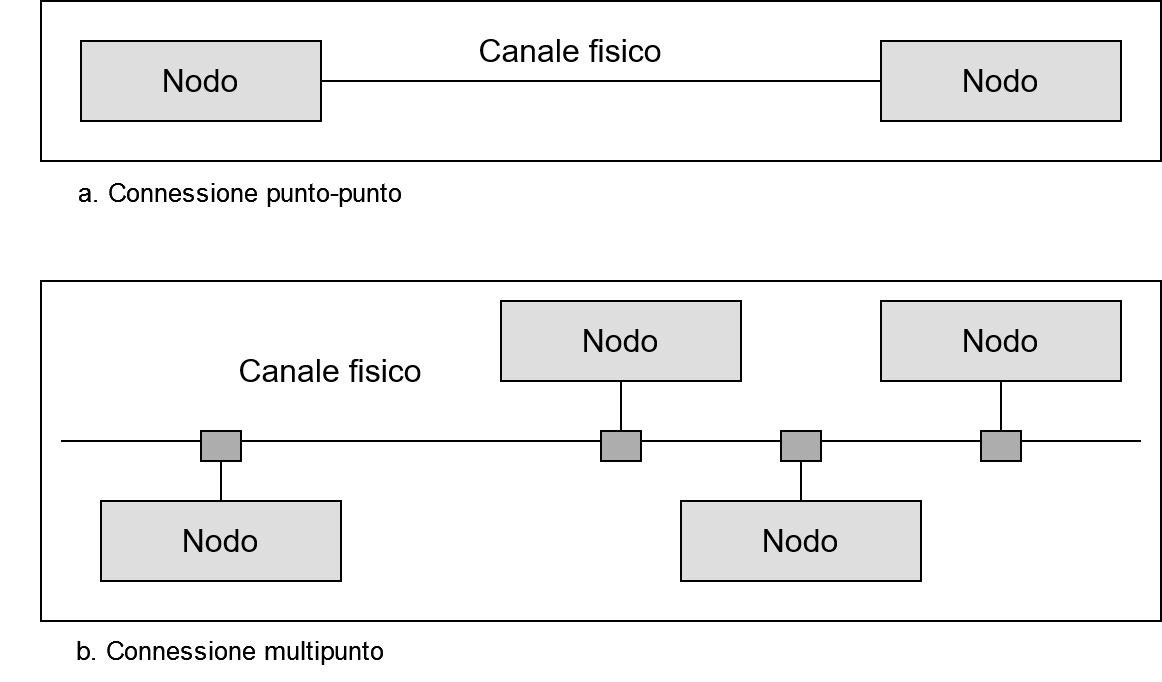
\includegraphics[width=0.8\textwidth]{img/img1.png}
                \caption{Differenza fra connessione punto-punto e multipunto.}
                \label{fig:img1}
            \end{figure}
            
        \newpage
        \subsubsection{Topologia}
            La topologia di una rete è il modo in cui i nodo sono fisicamente disposti e interconnessi. Essa è descritta dalla disposizione dei collegamenti, e quindi dei nodi, della rete. Esistono quattro tipi di topologie di base: mesh, stella, bus e anello.
            
            \paragraph{Mesh} In questa topologia ogni nodo ha un collegamento punto-punto con ogni altro nodo della rete. Il numero di collegamenti è quadratico nel numero dei nodi, sia usando collegamenti simplex che duplex.
            
            Le reti mesh sono usate con parsimonia, in quanto la manutenzione e l'installazione di nuovi nodi risultano dispendiose, a causa del grande numero di cavi.
            
            I vantaggi sono invece la grande interconessione; se un singolo collegamento diventa inusabile, ci sono molti altri cammini per trasferire i dati da un nodo all'altro. Questo chiaramente aumenta l'affidabilità e la sicurezza. Tuttavia dobbiamo notare che se un nodo è usato come punto di passaggio per parecchi cammini dati, il suo guasto potrebbe portare molti disagi.
            
            \begin{figure}[h]
                \centering
                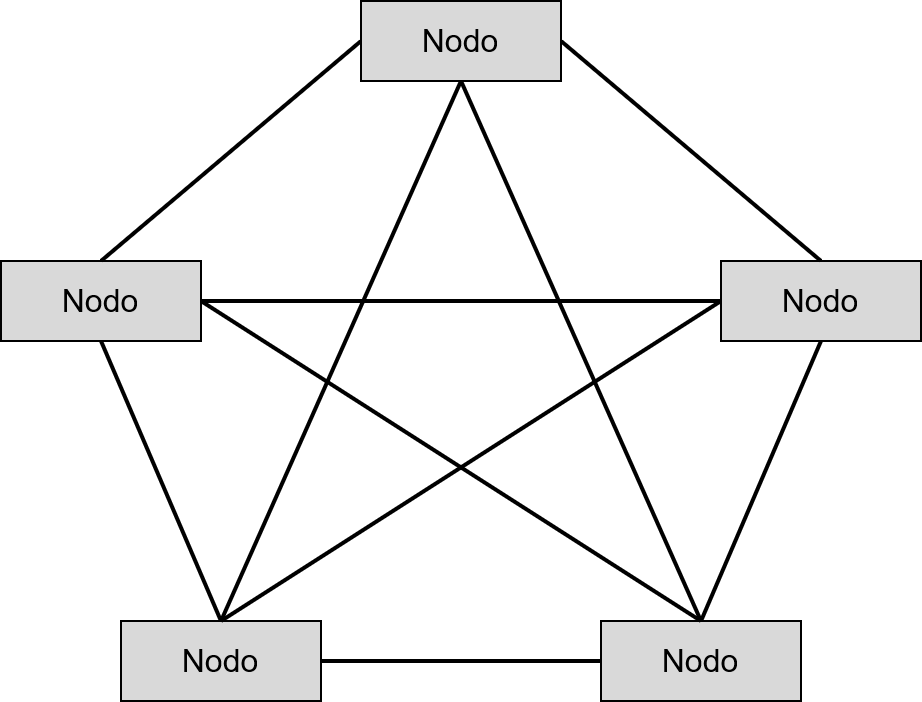
\includegraphics[width=0.45\textwidth]{img/mesh.png}
                \caption{Topologia mesh.}
                \label{fig:img1}
            \end{figure}
            
            \paragraph{Stella} Nella topologia a stella, ogni nodo è connesso tramite un collegamento punto-punto a un dispositivo centrale chiamato \textbf{hub}. Al contrario della topologia mesh, i nodi non possono essere in collegamento diretto fra di loro.
            
            Il vantaggio principale sta nel costo e nella manutenzione, in quanto il numero di porte I/O e collegamenti è lineare rispetto al numero dei nodi.
            
            Lo svantaggio principale sta nella presenza dell'hub, in quanto un suo guasto rischia di compromettere l'intera rete. Potrebbe inoltre fungere da collo di bottiglia per le prestazioni.
            
            \begin{figure}[h]
                \centering
                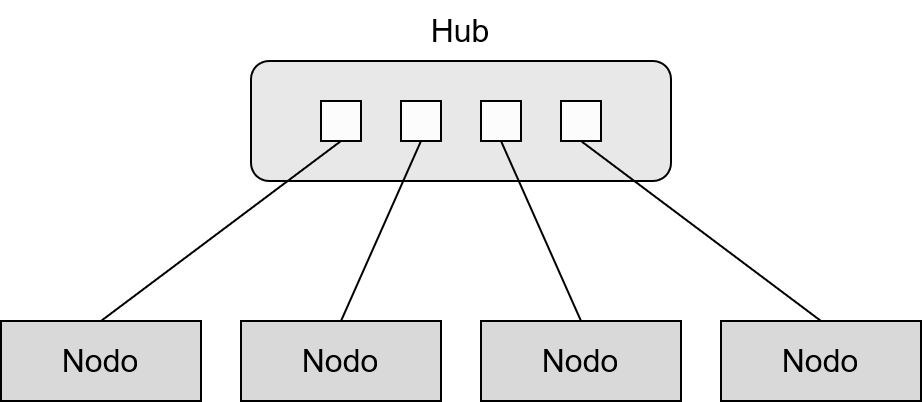
\includegraphics[width=0.55\textwidth]{img/stella.png}
                \caption{Topologia a stella.}
                \label{fig:img1}
            \end{figure}
            
            \newpage
            \paragraph{Bus} Questo tipo di rete utilizza un collegamento multipunto (il bus) che collega tutti i nodi della rete.
            
            Il problema principale è che il segnale diminuisce d'intensità attraversando il bus, e quindi questo non può essere molto lungo e quindi non può ospitare un grande numero di nodi.
            
            Il vantaggio principale sta nella semplice aggiunta di un nuovo nodo, che consta semplicemente nell'aggiunta di un connettore al bus. Tuttavia i nodi devono essere opportunamente distanziati e non creare rumore sul bus.
            
            \begin{figure}[h]
                \centering
                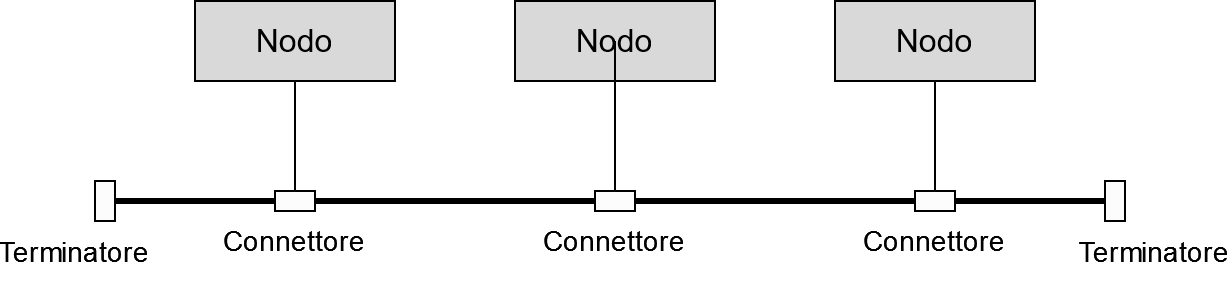
\includegraphics[width=0.70\textwidth]{img/bus.png}
                \caption{Topologia bus.}
                \label{fig:img1}
            \end{figure}
            
            \paragraph{Anello} In una tale topologia ogni nodo ha un collegamento punto-punto con soli altri due nodi: quello che lo segue e quello che lo precede nell'anello.
            
            I dati vengono fatti passare sull'anello in una sola direzione, e ogni anello ha un ripetitore che rigenera il segnale fino a che questo raggiunge la sua destinazione.
            
            La manutenzione e l'aggiunta di un nodo risultano abbastanza semplici. Quest'ultima richiede la modifica di due sole connessioni, quella precedente rispetto al nodo da aggiungere e quella successiva.
            
            Lo svantaggio principale sta nella natura unidirezionale della topologia: il guasto di un singolo collegamento rende non funzionante l'intera rete. Si può ovviare a questo problema usando un doppio anello.
            
            \begin{figure}[h]
                \centering
                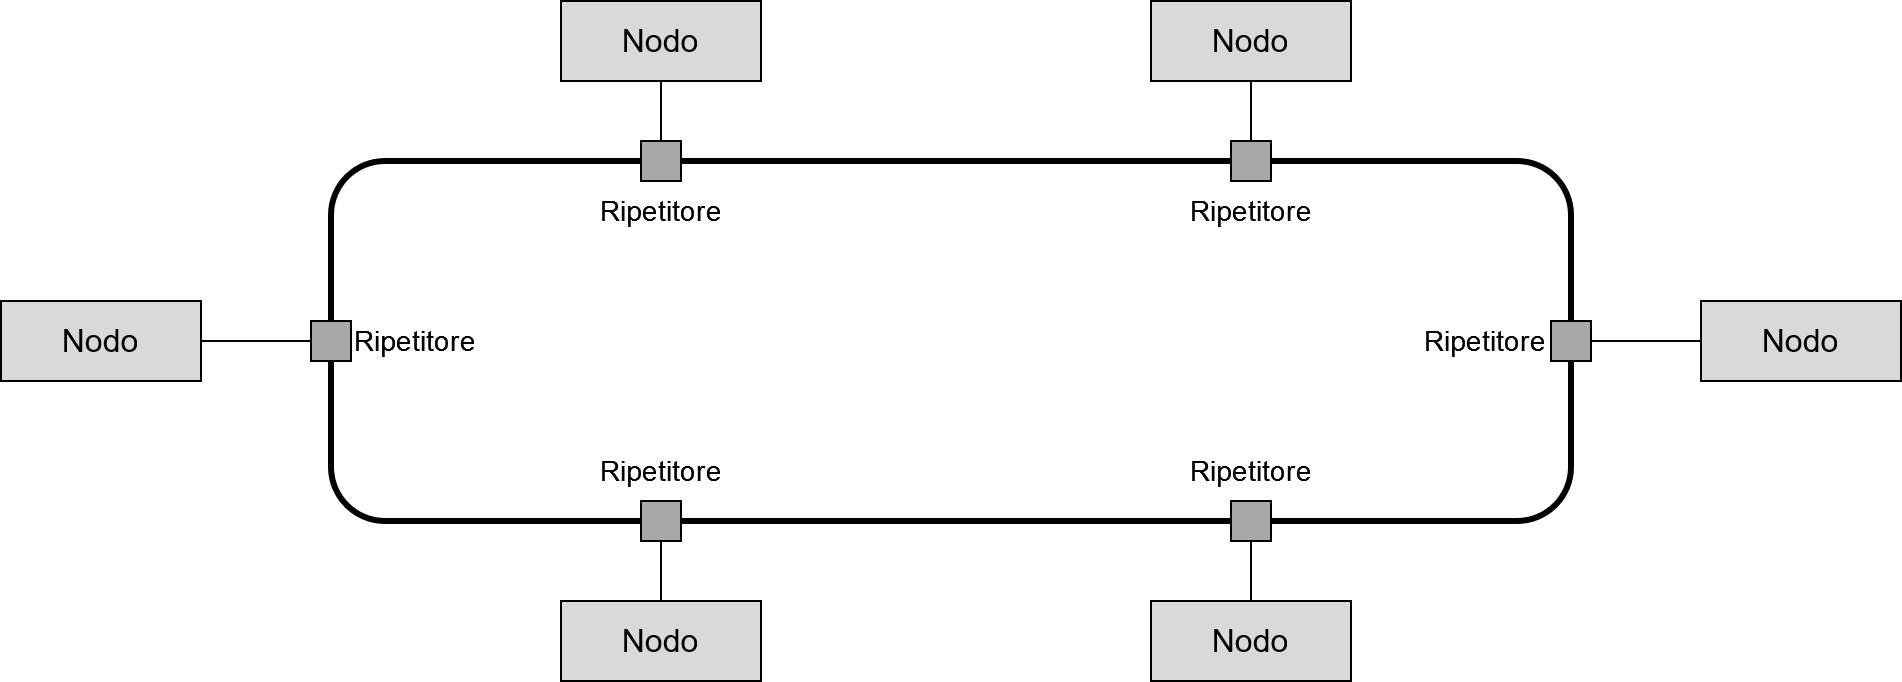
\includegraphics[width=1\textwidth]{img/anello.png}
                \caption{Topologia ad anello.}
                \label{fig:img1}
            \end{figure}
            
            \newpage
            \paragraph{Tipologia ibrida} Chiaramente si può costruire una rete unendo due o più topologie di base.
            
    \subsection{Modelli di rete}
        A causa della grande omogeneità di tecnologie usate per la costruzione di reti, necessitiamo di standard e protocolli per far comunicare due reti eterogenee. I due standard più conosciuti sono il modello OSI (Open System Interconnection) e il modello TCP/IP.
            
        Nel primo l'architettura di una rete è formata da sette livelli, mentre nel modello TCP/IP ne vengono usati cinque.
            
    \subsection{Classificazione delle reti}
        Le reti vengono classificate in base alle loro dimensioni fisiche. Le due categorie principali sono le LAN (Local Area Network) e le WAN (Wide Area Network). La prima ha una dimensione di solitamente non più di due chilometri, mentre la seconda può essere arbitrariamente grande, fino a coprire l'intero globo come accade per Internet. Reti intermedie sono chiamate MAN (Metropolitan Area Network), e spesso ricoprono l'area di un'intera città.
            
        \subsubsection{LAN}
            Una LAN può essere composta anche da soli due computer connessi fra loro, ma solitamente ricopre un edificio o un campus. Le LAN più estese possono collegare più edifici, magari di una stessa compagnia, e connettere dispositivi eterogenei come desktop, stampanti, etc.
                
            Le LAN sono progettate per condividere dati e risorse. Possiamo per esempio immaginare un computer che fa da server e offre accesso (eventualmente controllato) ad applicativi e dati.
                
            Il mezzo trasmissivo è solitamente omogeneo per tutta la rete, e le topologie più utilizzate sono quella a bus, ad anello e a stella.
                
        \subsubsection{WAN}
            Una tale rete mette in comunicazione dispositivi potenzialmente molto lontani, e può essere molto semplice, come nel caso di una connessione punto-punto fra due soli dispositivi, o molto complessa, come nel caso di Internet.
                
            Nel secondo caso di parla di rete WAN a commutazione e la rete è costituita da molti nodi speciali detti router, connessi fra di loro, che collegano le varie reti.
                
        \subsubsection{MAN}
            La dimensione di una Metropolitan Area Network si alloca fra quella di una LAN e di una WAN. Viene tipicamente usata per collegare i vari utenti di una regione, collocati in posizioni diverse, a una rete più grande, tipicamente Internet.
                
    \subsection{Interconnessioni di reti: interreti}
        Oggigiorno è raro trovare una WAN, LAN o MAN isolate da altre reti. Spesso le reti sono connesse ad altre reti, creando interreti o \textbf{internet}.
            
        Abbiamo definito una \textbf{internet} ("i" minuscola) come una qualsiasi rete costruita collegando più reti fra di loro. Ma \textit{Internet} con la "I" maiuscola è la interrete principale e permette a milioni di computer di connettersi fra loro e al World Wide Web.
            
        Storicamente, il protocollo TCP (Transmission Control Protocol) si occupava dello scambio di pacchetti dati, mentre il protocollo IP (Interent Protocol) di operazioni di livello più alto come frammentazione dei pacchetti, consegna affidabile e riassemblaggio. L'unione di questi due protocolli fece nascere il protocollo TCP/IP.
            
    \subsection{Protocolli e standard}
        Un \textbf{protocollo} è un insieme di regole. Affinché le sequenze di bit scambiate fra due nodi di una rete abbiano lo stesso significato per entrambi, serve seguire delle regole. Queste vengono chiamate appunto protocollo, e i suoi elementi chiave sono:
        \begin{itemize}
            \item \textbf{Sintassi.} Definisce il formato dei dati, ossia l'ordine in cui i vari elementi della comunicazione devono essere presentati.
            
            \item \textbf{Semantica.} Definisce il significato delle sequenze di bit.
            
            \item \textbf{Sincronizzazione.} Definisce due aspetti della comunicazione: quando i dati vengono inviati e a che velocità. Queste due caratteristiche devono coincidere altrimenti si rischia di creare un sovraccarico o di perdere dei bit.
        \end{itemize}
        
        Uno standard è comunque un insieme di regole, ma elaborate e approvate da un'organizzazione ufficialmente riconosciuta. Questo è utile se reti diverse o addirittura mutualmente sconosciute vogliono comunicare. Gli standard possono essere:
        \begin{itemize}
            \item \textbf{De facto.} Non sono stati approvati da nessuna organizzazione preposta per tale scopo, ma sono di fatto utilizzati.
            
            \item \textbf{De jure.} Sono stati approvati da un'organizzazione ufficialmente riconosciuta.
        \end{itemize}

\chapter{Capitolo 2: Modelli per le Reti}
Una rete è composta dall'hardware (computer, cavi), che permette di inviare una serie di bit da un nodo all'altro, che dal software, che permette di far assumere significato a questi bit e trasmettere un messaggio da un nodo a un qualsiasi altro nodo.

Per passare dai bit ai servizi di un software bisogna risolvere svariati problemi, ciascuno dei quali può essere inquadrato come appartenente a uno strato.

\section{Architettura a strati}
    Concettualmente immaginiamo un messaggio discendere dal mittente fra i diversi strati che lo codificano e decompongono, fino a spedirlo tramite il mezzo di comunicazione. Il destinatario farà risalire poi il messaggio attraverso gli stessi strati, ma in maniera inversa, quindi decodificandolo e ricomponendolo.
    
    Inoltre ogni strato offre un servizio allo strato superiore, e usa un servizio offerto dallo strato inferiore.
    
\section{Il modello OSI}
    Nonostante non sia stato usato a pieno perché surclassato da altri modelli, è un'ottima base per capire il funzionamento di un'architettura di rete a strati. È composto da sette livelli, ognuno dei quali definisce un particolare aspetto delle attività che servono per far muovere i dati sulla rete.
    
    \begin{figure}[h]
        \centering
        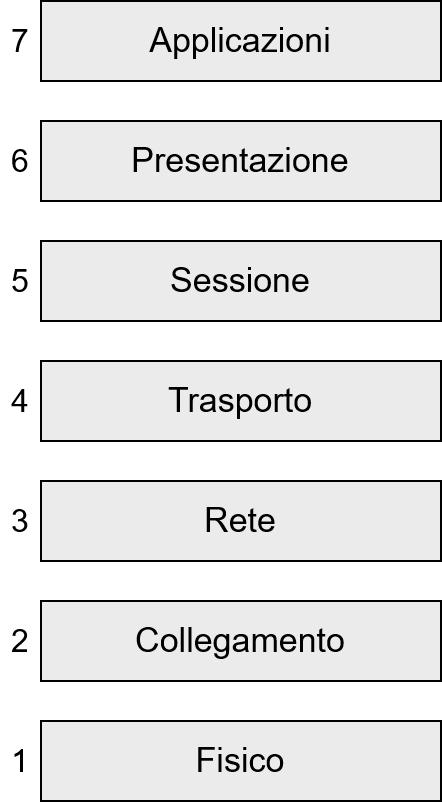
\includegraphics[width=0.33\textwidth]{img/strati_osi.png}
        \caption{I sette strati del modello OSI.}
        \label{fig:img1}
    \end{figure}
    
    Chiaramente ogni strato ha un'\textbf{interfaccia} che lo collega a quello precedente e a quello successivo. Questa interfaccia definisce quali servizi deve offrire allo strato sottostante e di quali può usufruire facendo riferimento allo strato superiore.
    
    Possiamo avere una serie di nodi intermedi nei tre stati più bassi (possiamo pensare a un mezzo fisico che non comunica direttamente col mezzo fisico di arrivo ma utilizza una serie di intermediari).
    
    Due livelli uguali di nodi diversi sono detti \textbf{peer}. La comunicazione fra due peer è detta peer-to-peer o p2p.
    
    \subsubsection{Organizzazione degli strati}
        I sette strati possono essere concettualmente divisi in tre gruppi:
        \begin{itemize}
            \item Gli \textbf{strati 1, 2, 3 (fisico, collegamento e rete)} sono strati per il supporto di rete, e hanno a che fare con le problematiche del mezzo fisico.
            
            \item Gli \textbf{strati 5, 6 e 7 (sessione, presentazione e applicazioni)} sono per il supporto all'utente, e permettono interoperabilità per sistemi che usano software diversi fra loro.
            
            \item Lo \textbf{strato 4 (trasporto)} collega i due gruppi sopra descritti.
        \end{itemize}
        
        Gli strati alti sono quasi sempre implementati in software, mentre gli strati bassi in un misto di hardware e software, tranne per lo strato fisico che è quasi sempre implementato quasi interamente in hardware.
    
    \subsection{Incapsulamento}
        Un aspetto importante della comunicazione dei dati del modello OSI è l'incapsulamento: il livello \textit{n} riceve dal livello \textit{n-1} un pacchetto di informazioni contenente sia i dati che l'header. Tuttavia i livelli più bassi non sanno niente dell'intestazione dei livelli più alti, e considerano l'intero pacchetto come un inseme unico di dati.
        
\newpage
\section{Strati del modello OSI}
    Qui descriveremo brevemente le funzioni di tutti gli strati del modello OSI.

    \subsection{Strato 1: Fisico}
        Deve tradurre la sequenza di bit nei segnali elettrici opportuni da inviare sul mezzo fisico. Gestisce le componenti meccaniche ed elettriche del mezzo trasmissivo.
        
        Per svolgere il suo compito deve avere a che fare con:
        \begin{itemize}
            \item \textbf{Caratteristiche fisiche dell'interfaccia e del mezzo trasmissivo.}
            
            \item \textbf{Rappresentazione dei bit.} Ossia come il valore 0 e il valore 1 sono codificati con i segnali da spedire sul mezzo trasmissivo.
            
            \item \textbf{Velocità di spedizione.} In altre parole, definisce quanto il segnale che rappresenta un bit deve durare (meno dura e maggiore è la velocità di spedizione).
            
            \item \textbf{Sincronizzazione dei bit.} Per una corretta lettura dei bit è necessario che il clock del mittenete e quello del destinatario siano sincronizzati.
            
            \item \textbf{Configurazione del collegamento.} La connessione del nodo al mezzo trasmissivo può essere punto-punto o multipunto.
            
            \item \textbf{Topologia.}
            
            \item \textbf{Flusso di dati.} Lo strato fisico definisce anche il tipo di comunicazione (simplex, half-duplex, duplex).
        \end{itemize}
        
    \subsection{Strato 2: Collegamento}
        Si occupa di varie problematiche fra cui correzione di errori; rende la trasmissione di pacchetti fra un nodo e l'altro affidabile. Deve avere a che fare con:
        \begin{itemize}
            \item \textbf{Framing.} Divide il flusso di bit che arriva dallo strato di rete e che deve essere spedito in blocchi, detti \textit{frame}.
            
            \item \textbf{Indirizzi fisici.} Se il destinatario è all'interno della stessa rete, nell'intestazione viene inserito il suo indirizzo fisico. Se è su un'altra rete, viene inserito l'indirizzo fisico del nodo che collega la rete corrente a un'altra rete.
            
            \item \textbf{Controllo di flusso.} Se le velocità di trasmissione e ricezione dei due nodi non sono in accordo, il flusso viene regolato per evitare un sovraccarico.
            
            \item \textbf{Controllo degli errori.} Permette di individuare i frame danneggiati e quindi di ritrasmetterli.
            
            \item \textbf{Controllo per l'accesso.} Quando il mezzo trasmissivo è multipunto, questo strato ha il compito di controllare quale nodo ha accesso al mezzo.
        \end{itemize}
        
        La comunicazione nello strato di collegamento avviene fra due frame successivi. Sia l'atto della trasmissione che i frame coinvolti vengono chiamati \textit{hop}.
        
    \subsection{Strato 3: Rete}
        Ha il compito di far arrivare il pacchetto di dati dal mittente al destinatario in una interrete, facendoli passare, se necessario, attraverso altre reti. Da ciò si evince che due nodi sulla stessa rete, per comunicare, non avranno bisogno dello strato di rete.
        
        Questo strato deve avere a che fare con:
        \begin{itemize}
            \item \textbf{Indirizzamento logico.} L'indirizzamento fisico non basta quando due nodi non sono sulla stessa rete. L'indirizzamento adeguato non dipende dalle componenti fisiche e si chiama indirizzamento logico.
            
            \item \textbf{Routing.} Quando più reti sono connesse fra di loro, i nodi che le connettono sono chiamati router. Il compito dello strato di rete è proprio di gestire questo meccanismo di routing.
        \end{itemize}
        
    \subsection{Strato 4: Trasporto}
        Si occupa della consegna di un messaggio da un processo mittente a un processo destinatario. Lo strato di rete non riconosce i pacchetti come appartenenti allo stesso messaggio, mentre lo stato di trasporto aggiunge questa logica, rendendo la fruizione del messaggio affidabile.
        
        Lo strato di collegamento deve avere a che fare con:
        \begin{itemize}
            \item \textbf{Indirizzamento dei processi.} Abbiamo visto che lo strato di rete si occupa di far giugnere i pacchetti al nodo destinatario. Lo strato di trasporto si occupa invece di smistare i pacchetti ai processi corretti. Questo tipo di meccanismo, che permette di distinguere fra i processi, viene chiamato indirizzo di servizio o di porta.
            
            \item \textbf{Segmentazione e riassemblaggio.} I singoli messaggi devono essere divisi in segmenti, ognuno dei quali contiene un numero di sequenza che permette il riassemblaggio una volta giunti a destinazione.
            
            \item \textbf{Controllo della connessione.} In una comunicazione senza connessione, i pacchetti vengono spediti in maniera indipendente l'uno dall'altro. Lo strato di trasporto offre invece una comunicazione con connessione, dove il mittente crea una connessione con lo strato di trasporto del destinatario prima di inviare i pacchetti contenenti i dati veri e propri. La connessione viene chiusa una volta che l'intero messaggio accordato è stato spedito.
            
            \item \textbf{Controllo del flusso.} Stavolta questo tipo di controllo avviene sui processi terminali, anziché sul mezzo di comunicazione come avviene per lo strato di collegamento.
            
            \item \textbf{Controllo degli errori.} Anziché operare sull'intero canale come in precedenza, si occupa della consistenza del messaggio scambiato fra i processi terminali.
        \end{itemize}
        
    \subsection{Strato 5: Sessione}
        Esso stabilisce, manitiene e sincronizza l'interazione fra i sistemi che comunicano. Le sue funzionalità sono:
        \begin{itemize}
            \item \textbf{Controllo del dialogo.} Permette a due sistemi, anche eterogenei, di comunicare.
            
            \item \textbf{Sincronizzazione.} Lo strato di sessione offre la possibilità ai processi di avere dei punti di controllo. Per esempio nell'invio di un messaggio da 1000 pagine, è opportuno controllare la corretta trasmissione ogni 100, così da diminuire l'eventuale numero di pagine da ritrasmettere.
        \end{itemize}
        
    \subsection{Strato 6: Presentazione}
        Si occupa di problematiche relative alla sintassi e alla semantica delle informazioni che devono essere trasmesse. Le sue funzionalità sono:
        \begin{itemize}
            \item \textbf{Traduzione.} Le informazioni di alto livello come il codice devono essere tradotte in sequenze di bit. Poiché diversi sistemi usano diversi schemi di codifica, queste differenze devono essere superate per permettere interoperabilità. Deve quindi essere usato un formato standard di rete, conversione che viene fatta dallo strato di presentazione.
            
            \item \textbf{Cifratura.} Nel mittente potrebbe avvenire una cifratura dei dati da spedire, cosa che richiederebbe poi una decifratura nello strato di presentazione del destinatario.
            
            \item \textbf{Compressione.}
        \end{itemize}
        
    \subsection{Strato 7: Applicazioni}
        Si occupa di fornire i servizi di rete all'utente finale, e comprende funzioni fra cui:
        \begin{itemize}
            \item \textbf{Terminale virtuale.} Un'emulazione del terminale del nodo remoto.
            
            \item \textbf{Gestione file.} Permette accesso e modifica di file da remoto.
            
            \item \textbf{Servizi di posta.} Permette lo scambio di messaggi elettronici fra utenti di una rete.
            
            \item \textbf{Servizi directory.}
        \end{itemize}
        
\section{La suite di protocolli TCP/IP}
    Gli strati di questa suite di protocolli non coincidono con quelli del protocollo OSI, in quanto sono stati sviluppati contemporaneamente, quando i secondi ancora non erano uno standard. Inizialmente ve ne erano quattro: strato nodo-rete, di rete, di trasporto e delle applicazioni. Lo strato nodo-rete comprende le funzionalità che nel modello OSI sono comprese nello strato fisico e in quello di collegamento, mentre lo strato delle applicazioni ingloba le funzionalità degli strati di sessione, presentazione e applicazioni del modello OSI.
    
    Definiremo il modello TCP/IP come composto da cinque strati che chiameremo fisico, di collegamento, di rete, di trasporto e delle applicazioni e che possono essere messi in corrispondenza con gli equivalenti strati del modello OSI, sebbene gli ultimi tre strati del modello OSI corrispondano a uno solo nel modello TCP/IP.
    
    La differenza principale fra il modello OSI e quello TCP/IP è che in quest'ultimo abbiamo strati strutturati gerarchicamente, nel senso che uno strato alto può essere supportato da uno o più strati bassi. Questo rende la struttura meno rigida e meno opaca.
    
    Per lo strato di trasporto TCP/IP definisce tre protocolli: TCP (Transmission Control Protocol), UDP (User Datagram Protocol) e SCTP (Stream Control Transmission Protocol). Per lo strato di rete il protocollo principale è IP (Internet Protocol).
    
    \subsection{Strati 1 e 2: fisico e di collegamento}
        Per questi strati il modello TCP/IP non definisce nessun protocollo, bensì supporta tutti i protocolli proprietari definiti dalle reti nelle quali TCP/IP viene utilizzato.
        
    \subsection{Strato 3: Rete}
        Come abbiamo detto, in questo strato viene definito il protocollo IP (Internet Protocol), che fa uso di quattro protocolli di servizio: ARP, RARP, ICMP e IGMP.
        
        \subsubsection{Protocollo IP}
            Il protocollo IP fornisce il servizio basilare di consegna pacchetti da un nodo all'altro nell'interrete. Il protocollo così definito è senza connessione e inaffidabile, un servizio detto \textit{best-effort}.
            
            Questo protocollo trasporta i dati in pacchetti detti \textit{datagram}, in maniera indipendente l'uno dall'altro. Come abbiamo detto, il protocollo IP non offre funzionalità per ovviare ai problemi a cui possono essere soggetti i \textit{datagram}, come arrivo non in ordine, perdita o duplicazione dei pacchetti. Nonostante ciò, esso offre funzionalità considerevoli in maniera abbastanza efficiente per le reti per le quali deve funzionare. Ulteriori accortezze nel suo funzionamento possono essere aggiunte usandolo semplicemente come base.
            
        \subsubsection{ARP (Address Resolution Protocol)}
            Il protocollo ARP permette di tradurre gli indirizzi logici usati dal protocollo IP per individuare i nodi nella interrete in in indirzzi fisici.
            
        \subsubsection{RARP (Reverse Address Resolution Protocol)}
            Questo protocollo permette di eseguire l'operazione inversa, ossia di risalire all'indirizzo IP logico a partire da quello fisico. Tipicamente viene usato quando il PC viene acceso e scoprire il suo indirizzo IP a partire dall'hardware.
            
        \subsubsection{ICMP (Internet Control Message Protocol)}
            Il protocollo ICMP viene usato per il controllo della rete. Quando si verifica un errore viene inviato un messaggio ICMP all'utente.
            
        \subsubsection{IGMP (Internet Group Message Protocol)}
            Esso offre delle funzionalità per la trasmissione simultanea di un messaggio a un gruppo di destinatari.
            
    \subsection{Strato 4: Trasporto}
        Mentre il protocollo IP permette di trasportare i pacchetti da un computer mittente a uno destinatario, i protocolli TCP e UDP permettono di trasportare i pacchetti da un processo mittente a un processo destinatario.
        
        È stato poi introdotto il protocollo SCTP per supportare alcune applicazioni recenti.
        
        \subsubsection{UDP (User Datagram Protocol)}
            È un protocollo molto semplice, che rispetto a IP introduce l'uso delle porte per l'identificazione dei processi, un codice per la rilevazione di errori e informazioni relative alla lunghezza dei dati provenienti dagli strati superiori.
            
        \subsubsection{TCP (Transmission Control Protocol)}
            Esso fornisce un servizio di trasporto affidabile fra processi orientato al flusso. Quindi questo protocollo stabilisce una connessione fra i punti terminali prima di spedire dati.
            
            Il mittente divide il flusso di byte da spedire in pezzi detti segmenti, ognuno dei quali ha un numero di sequenza che ne preserva l'ordine. Vengono poi passati al destinatario all'interno di datagram IP, che li riceverà prima di ordinarli.
    
    \subsection{Strato 5: Applicazioni}
        È equivalente alla combinazione degli strati di sessione, presentazione e applicazioni del modello OSI.

\chapter{Strato Fisico, Capitolo 3: Dati e Segnali}
\section{Dati e segnali analogici e digitali}
    Per essere trasmessi, i dati devono essere trasformati in segnali elettromagnetici.
    
    Sia i dati che i segnali che li rappresentano possono essere sia \textbf{analogici} che \textbf{digitali}.
    
    \paragraph{Dati analogici e digitali}
        I \textbf{dati analogici} sono informazione rappresentata in maniera continua; i \textbf{dati digitali} sono informazione rappresentata in maniera discreta.
        
    \paragraph{Segnali analogici e digitali}
        Come i dati che rappresentano, anche i segnali possono essere sia analogici che digitali. I segnali \textbf{analogici} possono assumere un infinito numero di valori di intensità, mentre quelli \textbf{digitali} ne possono assumere un numero limitato, che spesso è 1 o 0.
        
    \paragraph{Segnali periodici e aperiodici}
        Sia i segnali analogici che quelli digitali possono avere due forme: periodici e aperiodici. Un \textbf{segnale periodico} si ripete nel tempo a intervalli regolari. La forma che viene ripetuta viene chiamata \textit{ciclo}, mentre la durata di un singolo ciclo viene chiamata \textit{periodo}.
        
        Un \textbf{segnale aperiodico} invece non si ripete con regolarità nel tempo.
        
\section{Segnali analogici periodici}
    Questo tipo di segnali, insieme a quelli digitali aperiodici, sono molto usati nelle reti di calcolatori.
    
    Essi possono essere:
    \begin{itemize}
        \item \textbf{Semplici} (onde sinusoidali), se non possono essere decomposti in altri segnali.
        \item \textbf{Composti}, se invece possono essere decomposti ulteriormente in onde sinusoidali.
    \end{itemize}
    
    \subsection{Onde sinusoidali}
        È la più importante forma di segnale analogico periodico. Può essere rappresentata da tre parametri: ampiezza massima (o di picco), frequenza e fase. Questi tre parametri sono sufficienti per descrivere in modo completo l'onda.
        
        \subsubsection{Ampiezza massima}
            L'intensità massima, in valore assoluto, che il segnale raggiunge. È proporzionale all'energia trasportata dal segnale.
            
        \subsubsection{Periodo e frequenza}
            Il \textbf{periodo} è il tempo necessario, misurato in secondi, che il segnale impiega a completare un ciclo. La \textbf{frequenza} è invece il numero di cicli completati in un secondo. Si noti che essendo l'una l'inverso dell'altra, queste due misure descrivono la stessa caratteristiche di un segnale.
            \begin{center}
                $f = \frac{1}{T}$ \hspace{5mm} e \hspace{5mm} $T = \frac{1}{f}$
            \end{center}
            
            Mentre il periodo viene espresso in secondi, la frequenza viene spesso espressa in \textbf{hertz} (Hz), e rappresenta il numero di cicli per secondo.
            
    \subsection{Frequenza e velocità}
        Un altro modo di guardare la frequenza è misurare la velocità del segnale. Siccome un segnale della frequenza di 50Hz si ripete la metà delle volte di un segnale di frequenza 100Hz, possiamo dire che il primo è più "lento".
            
        La \textbf{velocità} è in pratica la velocità con cui un segnale cambia rispetto al tempo. Cambiamenti veloci implicano una frequenza alta.
            
        Consideriamo ora le situazioni \textbf{estreme}:
        \begin{itemize}
            \item Se un segnale \textbf{non cambia}, ossia rimane costante, la frequenza è 0. In questo caso il segnale non completa mai nemmeno un ciclo.
                
            \item Se invece un segnale cambia valore \textbf{istantaneamente}, la sua frequenza è infinita, in quanto il suo periodo è 0.
        \end{itemize}
            
        \subsubsection{Fase}
            Essa descrive la posizione dell'onda rispetto all'asse del tempo, e indica la posizione iniziale del primo ciclo. Viene definita in gradi o radianti.
            
    \subsection{Lunghezza d'onda}
        La lunghezza d'onda è un'altra caratteristica di un segnale, e mette in relazione il periodo, o la frequenza, con la velocità di propagazione del mezzo trasmissivo. Denotando con $\lambda$ la lunghezza d'onda e con $c$ la velocità di propagazione del segnale, si ha
        \begin{center}
            $\lambda = c \cdot T = \frac{c}{f}$
        \end{center}
        
        La lunghezza d'onda è spesso misurata in micrometri.
        
    \subsection{Segnali composti}
        Ci interessano le onde sinusoidali semplici perché sono ottime per trasportare segnali semplici, come l'energia elettrica o segnali d'allarme.
        
        Un'altra applicazione molto importante delle onde sinusoidali è comporle in segnali più complessi: agli inizi del '900, Fourier ha mostrato che un qualsiasi segnale composto è in realtà la somma di onde sinusoidali con varie frequenze, fasi e ampiezze.
        
        I segnali composti possono essere periodici o aperiodici; i componenti di un segnale composto \textbf{periodico} sono onde sinusoidali con frequenze discrete, mentre i componenti di un segnale composto \textbf{aperiodico} sono onde sinusoidali con frequenze continue.
        
    \subsection{Spettro e larghezza di banda}
        Lo spettro di un segnale è l'insieme delle frequenze che esso contiene. L'intervallo delle frequenze contenute in un segnale è detto \textbf{larghezza di banda}, ed è la misura fra la sequenza più alta e quella più bassa.
        
\section{Segnali digitali}
    Oltre a codificare le informazioni con un segnale analogico, possiamo anche usare un segnale digitale, per esempio associando il valore 1 a un voltaggio positivo e il valore 0 a un voltaggio nullo, per rappresentare i bit.
    
    Un segnale digitale può avere anche più di due livelli, e in generale ogni livello può codificare $\log_2L$ bit.
    
    \paragraph{Velocità}
        Solitamente si misura in bit per secondo, o \textit{bps}. È inversamente proporzionale alla durata del segnale che rappresenta un singolo bit.
        
    \subsection{Lunghezza dei bit}
        È l'analogo della lunghezza d'onda discusso in precedenza. Mentre la lunghezza d'onda può essere vista come la distanza che un ciclo occupa sul mezzo di trasmissione, la \textbf{lunghezza dei bit} è la distanza che un bit occupa sul mezzo trasmissivo.
        
    \subsection{Segnali digitali e segnali analogici composti}
        L'analisi di Fourier ci dice che un segnale digitale è un segnale analogico composto per il quale la larghezza di banda è infinita, in quanto i segmenti orizzontali denotano nessun cambiamento, mentre quelli verticali cambiamento istantaneo.
        
        Il segnale può essere scomposto quindi con l'analisi di Fourier, in frequenze discrete per un segnale periodico e in frequenze continue per un segnale aperiodico.
        
    \subsection{Trasmissione di segnali digitali}
        Ci occupiamo ora del problema della trasmissione di segnali digitali aperiodici. Essa può avvenire in due modi: trasmissione del segnale di base oppure trasmissione con modulazione del segnale.
        
        \subsubsection{Trasmissione del segnale di base}
            Questo metodo prevede di trasmettere il segnale senza modificarlo in un segnale analogico.
            
            Questo richiede dei canali \textbf{passa-basso}, ossia con una larghezza di banda che inizia da zero. Questo è possibile per un mezzo trasmissivo che collega direttamente due nodi, come un cavo che collega due PC, o per più PC un bus, con l'accortezza di farlo usare da un solo segnale alla volta.
            
        \subsubsection{Trasmissione con modulazione del segnale}
            Modulare un segnale digitale significa trasformarlo in un segnale analogico per poi essere trasmesso. Questo ci apre alla possibilità di usare dei canali \textbf{passa-banda}, ossia dei canali la cui larghezza di banda non inizia da 0.
            
\section{Deterioramento del segnale}
    C'è da considerare che il mezzo trasmissivo attraverso il quale i segnali viaggiano ne causa un deterioramento; i segnali in punto d'arrivo non sono identici a quelli generati dal mittente. Ci sono diversi tipi di deterioramento, e in particolare le cause principali sono l'attenuazione, la distorsione e il rumore.
    
    \subsection{Attenuazione}
        Questa è una perdita di energia, che è stata consumata per superare la resistenza del mezzo trasmissivo stesso. Per ovviare a questo problema vengono usati degli amplificatori che ripristinano il segnale.
        
        La variazione del segnale viene spesso misurata in \textbf{decibel} (dB).
        
    \subsection{Distorsione}
        La \textbf{distorsione} è un cambiamento della forma del segnale, ed è tipica dei segnali composti da varie frequenze. Siccome ogni segnale ha un suo ritardo nel mezzo trasmissivo, la differenza fra questi ritardi può creare differenze di fase nel segnale composto, che risulta in distorsione.
        
    \subsection{Rumore}
        Ci sono diversi tipi di rumore, con diverse cause e origini. Il rumore si traduce in segnale addizionale, non prodotto o inteso dal mittente, che si aggiunge al segnale inteso per la trasmissione.
        
        \begin{itemize}
            \item Il rumore \textbf{termico} è dato dal movimento casuale degli elettroni nel mezzo trasmissivo.
            
            \item Il rumore \textbf{indotto} arriva da sorgenti come per esempio motori che fungono da antenne trasmittenti, mentre il mezzo trasmissivo funziona come antenna ricevente.
            
            \item Il rumore \textbf{dovuto a interferenze} si ha quando due cavi sui quali vengono trasmesse informazioni sono sufficientemente vicini; i cavi agiscono, come prima, come antenne trasmittenti e riceventi.
            
            \item Il rumore \textbf{dovuto a impulsi} è causato da fonti esterne, come per esempio fulmini, che causano un cambiamento repentino del segnale.
        \end{itemize}
        
        \subsubsection{Rapporto segnale-rumore}
            Indichiamo il rapporto fra la potenza del segnale e la potenza del rumore come \textbf{SNR} (\textit{Signal to Noise Ratio}). Esso è dato da:
            
            \begin{center}
                SNR = potenza media del segnale / potenza media del rumore
            \end{center}
            
            Chiaramente vogliamo un valore alto, in quanto esso indica un segnale poco alterato dal rumore.
            
\section{Limiti di velocità per il trasferimento dati}
    Una considerazione molto importante che possiamo fare è relativa al limite teorico della velocità massima che possiamo raggiungere su un determinato mezzo di trasmissione: essa è relativa a tre fattori: la \textbf{larghezza di banda}, il \textbf{numero di livelli} del segnale e la \textbf{qualità} del segnale (ossia la quantità di rumore).
    
    \subsection{Canali senza rumore: Teorema di Nyquist}
        Il primo importante risultato teorico è questo teorema, che assume il caso ottimo di un canale senza rumore.
        \begin{center}
            Velocità in bit per secondo = 2 $\cdot$ larghezza di banda $\cdot \log_2L$
        \end{center}
        Dove L è il numero di livelli del segnale che possono essere usati per rappresentare i dati.
        
        Restando in ambito teorico è corretto dire che per ottenere una velocità di trasferimento maggiore basta aumentare L. Questo in pratica è poco fattibile in quanto introduciamo un problema per il ricevente: esso deve essere in grado di distinguere fra il maggior numero di livelli, il che richiede sia più sofisticato e introduce un certo livello di inaffidabilità nella trasmissione.
        
    \subsection{Canali con rumore: Teorema di Shannon}
        Nella pratica non esistono canali senza rumore. Shannon dimostrò un teorema per calcolare la \textbf{capacità}, ossia la velocità massima, di un canale con rumore.
        \begin{center}
            Capacità = larghezza di banda $\cdot \log_2(1 + SNR)$
        \end{center}
        
        Si noti che il numero di livelli non appare qui. Il teorema di shannon infatti definisce una caratteristica del canale, e non del metodo di trasmissione.
        
        I due teoremi appena visti non sono mutualmente esclusivi e anzi, nella pratica si usano in congiunzione per trovare velocità massima e numero di livelli da utilizzare.
        
\section{Prestazioni}
    Discutere delle prestazioni e dell'efficienza di una rete comporta la conoscenza di alcuni concetti e terminologie di base, che andremo ora a descrivere.
    
    \subsection{Larghezza di banda}
        Questo termine può essere usato con due accezioni:
        \begin{itemize}
            \item \textbf{Larghezza di banda in hertz:} come abbiamo già discusso, rappresenta l'intervallo di frequenze contenute in un segnale.
            
            \item \textbf{Larghezza di banda in bit per secondo:} questa rappresenta invece la velocità massima alla quale possiamo spedire informazioni su un certo canale trasmissivo.
        \end{itemize}
        
    \subsection{Throughput}
        Il \textbf{throughput} è la velocità alla quale possiamo spedire dati attraverso una rete. Sebbene possa sembrare simile alla larghezza di banda in bps, è una misura diversa. È infatti una misura più pratica, che prende in considerazione per esempio eventuali nodi bottleneck.
        
    \subsection{Latenza (Ritardo)}
        La latenza è il tempo necessario perché un intero messaggio arrivi a destinazione. Essa viene misurata a partire da quando il primo bit viene inviato dal mittente e si conclude quanto l'ultimo bit viene recepito dal destinatario.
        
        Possiamo dire che la latenza è composta da quattro fattori:
        \begin{center}
            Latenza = tempo di propagazione + tempo di trasmissione + tempo di attesa + tempo di inoltro
       \end{center}
       
       \subsubsection{Tempo di propagazione}
            È il tempo necessario al segnale per viaggiare dal mittente al destinatario.
            \begin{center}
                $\text{Tempo di propagazione} = \frac{\text{distanza}}{\text{velocità di propagazione}}$
            \end{center}
            
        \subsubsection{Tempo di trasmissione}
            Normalmente spediamo un insieme di bit; per il primo dobbiamo aspettare che questo arrivi a destinazione, ma i successivi saranno accodati e quindi non richiederanno un'ulteriore attesa. Il tempo di trasmissione è il tempo necessario a inserire i bit del messaggio sul mezzo trasmissivo.
            \begin{center}
                $\text{Tempo di trasmissione} = \frac{\text{dimensione del messaggio (in bit)}}{\text{larghezza di banda (in bit)}}$
            \end{center}
            
        \subsubsection{Tempo di attesa}
            Questo è dato dai tempi di attesa nelle code dei nodi intermedi. Non è un valore fisso, in quanto varia in base al carico della rete.
            
        \subsubsection{Tempo di inoltro}
            Questo tempo dipende comunque dai nodi intermedi e dalla velocità con cui inoltrano i messaggi, ma non è dipendente dal carico della rete; bensì dalle caratteristiche hardware dei nodi intermedi.
            
    \subsection{Prodotto banda-ritardo}
        Nonostante i valori di larghezza di banda e di latenza siano importanti, ancora più importante è il loro prodotto; esso ci dice quanti bit possiamo spedire su un certo canale per riempirlo. Spedirne di meno sarebbe poco efficace, mentre spedirne di più causerebbe una perdita di dati.

\chapter{Strato Fisico, Capitolo 4: Trasmissione Dati}
Una rete di comunicazione è progettata con lo scopo di trasferire dati da un punto all'altro. Siccome i dati possono essere in forma digitale o analogica, deve esserci corrispondenza fra la rappresentazione dei dati e il tipo di dati che il canale trasmissivo è adatto a trasportare.

Per questo motivo discutiamo di conversioni analogico-digitale e digitale-analogico. Tuttavia potremmo aver bisogno di convertire un segnale da digitale in digitale per esempio, se le due larghezze di banda usate per rappresentarlo sono diverse, o da analogico in analogico.

\section{Conversione digitale-digitale}
    Vediamo varie tecniche per rappresentare dati digitali con segnali digitali. Vediamo la codifica di linea, sempre necessaria, e le codifiche a blocchi e scrambling, non necessarie.
    
    \subsection{Codifica di linea}
        La codifica di linea è il processo di convertire dati digitali, che assumeremo memorizzati come sequenze di bit, in segnali digitali.
        
        L'\textbf{unità di base dei dati} è il più piccolo elemento che rappresenta informazioni, ossia il bit. Analogamente, l'\textbf{unità di base dei segnali} si chiamerà elemento del segnale, ed è il più piccolo elemento trasmissibile sul canale. Chiaramente gli elementi del segnale devono rappresentare gli elementi dei dati.
        
        Un dato importante è il \textbf{rapporto di elementi dei dati rappresentati da ogni elemento del segnale}. Un elemento del segnale potrebbe rappresentare, nel caso più semplice, un solo bit, nel qual caso $r = 1$. Questo valore potrebbe non coincidere con 1 nel caso in cui per rappresentare un singolo bit siano necessari più elementi del segnale, o nel caso in cui ogni elemento del segnale rappresenti più bit.
        
        \paragraph{Velocità dei dati e velocità del segnale} La velocità dei dati è la quantità di unità di base dei dati che possono essere spediti in un secondo, e viene misurata in bit per secondo, o bps. La velocità del segnale ha misura analoga e si misura in \textbf{baud}. Il nostro scopo è di riuscire ad ottenere una velocità dei dati quanto più alta possibile senza necessariamente aumentare troppo quella dei segnali. Vogliamo, in pratica, riuscire a trasportare più dati con meno segnali.
        
        \paragraph{Linea di base} Durante la decodifica di un segnale digitale, il ricevente calcola in tempo reale la media della potenza del segnale che riceve. Questa è chiamata linea di base. I valori nuovi vengono confrontati con la linea di base per stabilirne il valore. Una lunga sequenza di valori uguali può causare uno spostamento della linea di base e rendere più difficoltosa la decodifica, e questo è da considerare durante la progettazione di uno schema di codifica.
        
        \paragraph{Componenti DC} Quando il voltaggio di un segnale digitale è costante per molto tempo, vengono usati voltaggi molto bassi per trasmetterlo. Queste frequenze vicino a zero vengono chiamate componenti a corrente diretta (DC Component), e questo è da tenere in considerazione, in quanto alcuni sistemi non permettono il passaggio di frequenze particolarmente basse. Occorrono quindi schemi di codifica che impediscano a una lunga sequenza di bit uguali di essere spediti (in un caso banalmente semplice possiamo pensare di codificare 0 con 01 e 1 con 10).
        
        \paragraph{Sincronizzazione automatica} Per avere una sincronizzazione dei segnali inviati e di quelli ricevuti, i clock del mittente e del destinatario devono corrispondere. Un segnale auto-sincronizzante spedisce, insieme alle solite informazioni, delle informazioni relative al tempo vengono aggiunte. Queste possono essere specifiche sequenze di segnali che indicano l'inizio, la fine o qualsiasi altro punto di un gruppo di bit.
        
    \subsection{Schemi di codifica di linea}
        \subsubsection{Schemi unipolari}
            In uno schema unipolare, tutti i valori di tutti i livelli del segnale sono o positivi o negativi, ossia hanno lo stesso segno. In questo caso consideriamo lo 0 sia come positivo che come negativo.
            
            \paragraph{NRZ} Questa codifica, Non-Return-to-Zero, rappresenta il valore 1 con un voltaggio positivo e il valore 0 con un voltaggio nullo. Rispetto alla sua controparte polare è piuttosto costosa.
            
        \subsection{Schemi polari}
            In questo schema, i livelli possono assumere sia valori positivi che negativi. Possiamo per esempio un valore negativo per rappresentare 1 e un valore positivo per rappresentare 0.
            
            \paragraph{NRZ Polare} In questo schema vengono usati due livelli, uno positivo e uno negativo. Ne esistono due versioni:
            \begin{itemize}
                \item Nella versione \textbf{NRZ-Level}, o NRZ-L, il livello del voltaggio determina il valore del bit; un voltaggio positivo rappresenta il bit 1, uno negativo rappresenta il bit 0.
                
                \item Nella versione \textbf{NRZ-Invert}, o NRZ-I, l'entità del bit è rappresentata dalla presenza o meno di un cambiamento. Se il voltaggio cambia il bit è 1, se resta invariato è 0.
            \end{itemize}
            
            Nella versione L, la linea di base converge a uno dei due valori per lunghe sequenze di bit uguali, siano essi 1 o 0. La versione I è invece più resistente, in quanto riscontra questo problema solo per lunghe sequenze di zeri.
            
            Un secondo problema sta nella sincronizzazione. Mentre per lo schema NRZ-L è difficile sincronizzare i due clock per lunghe sequenze di bit uguali, per lo schema NRZ-I ciò avviene, come prima, solo per lunghe sequenze di zeri.
            
            Lo schema NRZ-L soffre, anche in questo caso, più della controparte Invert, nel caso di cambi di polarità. In tali casi tutti gli zeri diventano uni e viceversa, cosa che per lo schema Invert non crea alcun problema.
            
            \paragraph{RZ} Lo schema Return-to-Zero risolve il problema della sincronizzazione dei clock usando tre livelli del segnale: uno positivo, uno negativo e uno uguale a zero. Questo schema usa un voltaggio positivo per rappresentare 1 e uno negativo per rappresentare 0, ma torna poi a zero fino all'inizio della trasmissione del prossimo bit. Questo ritorno a zero può essere usato come elemento di sincronizzazione. Siccome per rappresentare un bit sono necessari due cambiamenti del segnale, questa codifica è meno efficiente (richiede una larghezza di banda maggiore). Inoltre, nonostante non soffra di problemi relativi alle componenti DC, riscontra difficoltà con l'inversione di polarità.
            
            \paragraph{Codifiche bifase} L'idea della transizione al centro di ogni bit combinata con lo schema NRZ-L, produce la \textbf{codifica Manchester}. Ogni bit è rappresentato da due cambiamenti di voltaggio, e in particolare il bit 0 è rappresentato da un cambiamento da voltaggio positivo a negativo, mentre il bit 1 da un cambiamento da voltaggio negativo a positivo.
            
            L'idea del cambiamento al centro di ogni bit combinata invece con la codifica NRZ-I, produce lo schema \textbf{Manchester differenziale}. Anche in questo caso abbiamo un cambiamento di voltaggio per ogni bit, ma anziché determinare l'entità del bit, determina la presenza di un cambiamento; la presenza di una transizione all'inizio dell'intervallo rappresenta un cambiamento di bit, e viceversa. Il problema principale di queste codifiche è che è richiesta una velocità doppia per implementarle. Tuttavia non riscontriamo problemi relativi alle componenti DC, alla sincronizzazione o alla linea di base.
            
        \subsubsection{Codifiche bipolari}
            Negli schemi di codifica bipolare vengono usati tre valori; uno uguale a zero, uno positivo e uno negativo.
            
            \paragraph{Codifiche AMI e pseudoternaria} La codifica \textbf{AMI} (Alternate Mark Inversion) rappresenta il valore zero con il voltaggio nullo e il valore uno con voltaggi positivi e negativi che si alternano. La codifica \textbf{pseudoternaria} rappresenta i valori in maniera opposta: zero è rappresentato da voltaggi positivi e negativi che si alternano, mentre uno è rappresentato dal voltaggio nullo.
            
            Le codifiche bipolari sono state sviluppate come alternativa allo schema NRZ; infatti la loro velocità è uguale, ma non abbiamo componenti DC, in quanto per valori positivi il voltaggio si alterna fra positivo e negativo, mentre per valori zero il voltaggio è nullo, il che non comporta un problema nel contesto delle componenti DC.
            
            I problemi di sincronizzazione rimangono; in futuro vedremo come ovviarvi tramite tecniche di scrambling.
            
        \subsubsection{Codifiche multilivello}
            Queste si sono rese necessarie nel caso, abbastanza comune, in cui abbiamo bisogno di inviare più dati, o in cui abbiamo bisogno di inviarne gli stessi una minore larghezza di banda.
            
            \paragraph{2B1Q} Questa tecnica codifica sequenze di due bit con un elemento di segnale a quattro livelli. Il destinatario deve chiaramente essere capace di distinguere fra i quattro segnali. Non ci sono livelli del segnale inutilizzati.
            
    \subsection{Codifica a blocchi}
        Per fornire una certa protezione dagli errori e uno strumento di sincronizzazione, è necessario introdurre una certa ridondanza. La codifica a blocchi fa proprio questo, trasformando una \textit{parola sorgente} di \textit{n} bit in una \textit{parola ccodice} di \textit{m} bit, con $m > n$. Le codifiche prendono il nome di \textit{nB/mB}, con valori di $n$ ed $m$ opportuni.
        
        \paragraph{4B/5B} Questa codifica è stata progettata per essere usata con lo schema di codifica di linea NRZ-I. Suddetto schema ha un problema di sincronizzazione, e in particolare, con lunghe sequenze di zeri non si ha un punto di riferimento. La codifica 4B/5B non permette mai la presenza di più di tre 0 consecutivi, risolvendo questo problema, ma non quello delle componenti DC.
    
\section{Conversione analogico-digitale}
    Nel mondo delle comunicazioni la chiara tendenza è quella di lavorare con segnali quanto più possibile digitali. Andiamo quindi a vedere metodi per convertire dati analogici (come il suono di un microfono o il segnale ottico di una videocamera) in dati digitali, che possiamo poi inviare tramite una delle tecniche precedentemente viste.
    
    \subsection{Modulazione a impulsi codificati}
        Questa tecnica, detta anche PCM (Pulse Code Modulation) è la tecnica più comune per convertire dati analogici in segnali digitali. I tre passi che esegue sono:
        \begin{itemize}
            \item Il segnale originale viene \textbf{campionato}, cioè misurato a intervalli regolari.
            
            \item Il segnale viene \textbf{quantizzato}, ossia rappresentato attraverso un insieme finito di valori.
            
            \item Il risultato della quantizzazione viene \textbf{codificato} tramite una sequenza di bit.
        \end{itemize}
        
        \subsubsection{Campionamento}
            Nel \textbf{campionamento ideale}, gli impulsi del segnale analogico vengono misurati in precisi istanti spaziati fra loro in maniera regolare. Questo tuttavia è difficile da implementare, e si ricorre al \textbf{campionamento naturale}, che misura gli impulsi del segnale analogico per brevi intervalli che includono l'istante di campionamento ideale. La tecnica più comune tuttavia è il campionamento a gradini, che è simile al campionamento naturale ma produce valori costanti.
            
            Per quanto riguarda la \textbf{velocità di campionamento}, dal teorema di Nyquist possiamo ricavare che per ottenere un segnale fedele a quello originale, bisogna campionarlo con una frequenza doppia rispetto alla massima frequenza raggiunta dal segnale.
            
        \subsubsection{Quantizzazione}
            Il risultato della fase di campionamento sono una serie di impulsi rappresentati da valori reali che spaziano dall'ampiezza minima a quella massima. Tuttavia essi vanno approssimati a valori discreti. Ciò avviene nel seguente modo:
            \begin{itemize}
                \item Si individuano $V_{min}$ e $V_{max}$ valori minimi e massimi dell'ampiezza del segnale.
                
                \item L'intervallo $[V_{min}, V_{max}]$ viene diviso in L intervalli di ampiezza $\Delta$. Il valore scelto per L determina la precisione della quantizzazione.
                
                \item Ogni intervallo viene rappresentato da un valore di quantizzazione compreso fra 0 e L-1.
                
                \item La misura del campionamento viene approssimata con il valore di quantizzazione del corrispondente intervallo.
            \end{itemize}
            
            Il valore di L varia in base all'ampiezza del segnale da rappresentare e dalla precisione che vogliamo ottenere. Un segnale che varia fra soli due valori è ben rappresentabile da una L pari a 2, ma un segnale più complesso come la voce umana ha bisogno di una L più alta, comunemente nell'ordine delle centinaia. Un segnale video ha una L nell'ordine delle migliaia.
            
            L'\textbf{errore di quantizzazione} dipende dal numero di livelli usati, e varia da $-\Delta/2$ a $\Delta/2$. Questo causa una riduzione del rapporto SNR, causando quindi una riduzione della capacità del canale.
            
        \subsubsection{Codifica}
            Siccome i valori di quantizzazione spaziano da 0 a L-1, possiamo semplicemente rappresentarli con i rispettivi valori binari. Chiaramente per L livelli saranno necessari $\log_2L$ bit. La velocità necessaria per per rappresentare il segnale campionato è data dalla formula
            \begin{center}
                Velocità dei dati = velocità di campionamento $\times$ numero di bit per campione
            \end{center}
            
        \subsubsection{Ripristino del segnale originale}
            Il segnale originale può essere ripristinato tramite un decodificatore PCM, che convertirà i bit ricevuti in impulsi per poi applicare un filtro passa basso, così da rendere più fluido il segnale. Se è stata usata una frequenza di campionamento di almeno il doppio della frequenza massima del segnale e se L è abbastanza alto, il segnale riprodotto sarà perfettamente fedele a quello originale.
            
\section{Modalità di trasmissione}
    Possiamo avere diversi tipi di connessioni fra dispositivi, suddivise in base a quanti cavi li collegano. Un singolo cavo può trasmettere un solo bit per volta, mentre più fili possono trasmettere più bit parallelamente.
    
    \subsection{Trasmissione parallela}
        Questo metodo di trasmissione permette di suddividere i bit da inviare in gruppi di n bit ciascuno, da inviare su n cavi.
        
        Questo metodo di trasmissione, a parità di tutti gli altri parametri, è più veloce ma più costoso, motivo per cui viene usato solo per brevi distanze.
        
    \subsection{Trasmissione seriale}
        Questo tipo di trasmissione è più lenta, in quanto invia i bit uno alla volta, ma anche meno costosa. Si può classificare in sincrona, asincrona e isincrona.
        
        \paragraph{Trasmissione seriale asincrona}
            In questo tipo di trasmissione seriale, la sincronizzazione del segnale non è importante. Il destinatario riuscirà a interpretare i bit arrivati indipendentemente dalla velocità con cui arrivano. Questo significa anche che non è prevedibile quando il prossimo bit arriverà, e ciò va segnalato. Può essere usato per esempio un bit addizionale all'inizio di ogni byte. Questo bit, che solitamente è 0, viene chiamato \textbf{bit di start}. Analogamente possono essere usati uno o più \textbf{bit di stop} per segnalare la fine di un gruppo di bit. Fra due byte consecutivi può esserci un'assenza di trasmissione, segnalata da un'assenza di segnale o da un flusso continuato di bit di stop.
            
            Queste accortezze di sincronizzazione a livello di bit ma non di byte rendono la trasmissione piuttosto lenta. Tuttavia resta comunque appetibile, soprattutto in casi in cui non ci interessa una velocità molto elevata. Per esempio nella trasmissione di dati digitati su una tastiera all'unità centrale di un computer, la velocità di digitazione è lenta relativamente a quella di trasmissione e il ritardo fra un carattere e l'altro è imprevedibile.
            
        \paragraph{Trasmissione seriale sincrona}
            In questo tipo di trasmissione, il pacchetti di bit di base viene chiamato \textbf{frame}, il quale può contenere anche molti byte. Essi vengono spediti come un flusso continuo di 0 e 1, e sta al destinatario dividerli correttamente in byte.
            
            Questo tipo di trasmissione è chiaramente più veloce ma richiede un maggior lavoro di sincronizzazione, che viene risolto nello strato di collegamento. È anche bene sottolineare che nonostante non ci siano periodi di mancanza di segnale all'interno del frame, potrebbero essercene fra un frame e il prossimo.
            
        \paragraph{Trasmissione seriale isincrona}
            Garantisce l'arrivo dei dati a una velocità costante. Molto utile per streaming di dati multimediali, per i quali variazioni di ritardo fra i pacchetti di dati non sono accettabili.
            
\section{Conversione digitale-analogico}
    Abbiamo visto che tre parametri descrivono un'onda sinusoidale: ampiezza, frequenza e fase. Per rappresentare segnali digitali, possiamo far variare uno di questi tre parametri. Questo ci offre tre diversi meccanismi per la modulazione di dati digitali in un segnale analogico: la \textbf{modulazione ASK} (Amplitude Shift Keying) che varia l'ampiezza, la \textbf{modulazione PSK} (Pulse Shift Keying) che varia la fase, e la \textbf{modulazione FSK} (Frequency Shift Keying) che varia la frequenza. Un quarto meccanismo varia sia l'ampiezza che la fase.
    
    \subsection{Aspetti della conversione digitale-analogico}
        Nella trasmissione analogica, il dispositivo mittente produce un segnale ad alta frequenza che serve come riferimento pere il segnale che trasporta l'informazione. Questo segnale viene chiamato \textbf{segnale} o \textbf{frequenza portante}. Il destinatario si sintonizza si questa frequenza, e le informazioni vengono trasmesse variando il segnale rispetto a una delle tre caratteristiche di un'onda sinusoidale. Questo tipo di modifica viene chiamata modulazione.
        
    \subsection{Modulazione ASK}
        In questo tipo di modulazione viene variata l'ampiezza, lasciando frequenza e fase invariati.
        
        \subsubsection{Modulazione ASK binaria (BASK)}
            Questa tecnica prevede due livelli del segnale, nonostante un elemento del segnale analogico possa assumere molte ampiezze diverse. Le due forme comunemente utilizzate sono una con ampiezza nulla, l'altra con ampiezza uguale a quella massima del segnale portante. Questi due valori dell'ampiezza possono rappresentare i due valori dei bit.
            
            Per quanto riguarda la \textbf{larghezza di banda}, essa è proporzionale alla velocità del segnale, ma dipende anche da un valore $d$ che è dato da aspetti relativi alla modulazione e al filtraggio. La banda utilizzata è importante, in quanto possiamo scegliere la frequenza portante, la quale vi si troverà al centro. Questo non è un problema in quanto l'ampiezza varierà fra questa frequenza portante e un'ampiezza nulla.
            
    \subsection{Modulazione FSK}
        Per la modulazione FSK varia la frequenza, mentre ampiezza e fase restano costanti.
        
        \subsubsection{Modulazione FSK binaria (BFSK)}
            Questo tipo di modulazione utilizza due frequenze portanti, normalmente molto alte e molto vicine. Una delle due viene usata per il valore 0, l'altra per il valore 1.
            
    \subsection{Modulazione PSK}
        Questo tipo di modulazione viene variata la fase del segnale, lasciando invariate frequenza e ampiezza.
        
        \subsubsection{Modulazione PSK binaria (BPSK)}
            Nella versione binaria, si hanno due tipi di segnali, uno con fase di $0^{\circ}$, e l'altro con fase di $180^{\circ}$. Questo tipo di modulazione è più resistente al rumore rispetto a quella in ampiezza, e inoltre non ha bisogno di due segnali portanti al contrario della FSK, ma ne mantiene la semplicità.
            
    \subsection{Quadratura PSK (QPSK)}
        Questa versione della PSK utilizza quattro diverse fasi, potendo quindi usare due bit per ogni elemento del segnale.
        
\section{Conversione analogico-analogico}
    Questo tipo di modulazione può essere necessaria se il canale a disposizione è passa-banda per esempio. Possiamo modulare l'ampiezza (\textbf{Amplitude Modulation}, AM), la frequenza (\textbf{Frequency Modulation}, FM) o la fase (\textbf{Phase Modulation}, PM).
    
    \subsection{Modulazione di ampiezza (AM)}
        L'ampiezza del segnale modulato varia al cambiare dell'ampiezza del segnale modulante, mentre frequenza e fase restano invariati. Si usa spesso un semplice moltiplicatore per ottenere questo effetto.
        
    \subsection{Modulazione di frequenza (FM)}
        Nella trasmissione in modulazione di frequenza invece, la frequenza del segnale portante viene modulata per rappresentare i cambiamenti dell'ampiezza del segnale originale, o modulante.
        
    \subsection{Modulazione di fase (PM)}
        Mentre la frequenza e l'ampiezza restano invariate, la fase del segnale portante rappresenta l'ampiezza del segnale originale. Questa modulazione è equivalente alla modulazione in frequenza, solo con la differenza che mentre nella FM i cambiamenti del segnale portante sono proporzinali all'ampiezza del segnale modulante, nella PM sono proporzionali alla sua derivata.

\chapter{Strato Fisico, Capitolo 5: Multiplexing e Diffusione}
Nella pratica ci troviamo a operare con una larghezza di banda limitata. Per utilizzarla in maniera coerente ed efficace dobbiamo introdurre due concetti: il \textbf{multiplexing}, che mira a utilizzare tutta la banda combinando più canali in uno solo, e la \textbf{diffusione}, il cui obiettivo è espandere la larghezza di banda per introdurre la ridondanza necessaria a evitare errori ed interferenze.

\section{Multiplexing}
    Il problema principale a cui il multiplexing cerca di ovviare è l'utilizzo di una canale trasmissivo che mette a disposizione una larghezza di banda troppo grande per il segnale che deve essere inviato.
    
    In un sistema che usa multiplexing, $n$ linee (trasmissioni) condividono un unico canale di trasmissione fisico. Esse verranno combinate in un'unico segnale prima di essere inviate da un \textbf{multiplexer} (\textbf{MUX}). Una volta arrivate a destinazione un \textbf{demultiplexer} (\textbf{DEMUX}) riconvertirà il segnale negli $n$ originali.
    
    Esistono tre tecniche per eseguire il multiplexing, basate rispettivamente sulla frequenza, sulla lunghezza d'onda e sul tempo. Le prime due sono progettate per funzionare con segnali analogici, mentre la terza con segnali digitali.
    
    \subsection{Multiplexing a divisione di frequenza}
        Il \textbf{multiplexing a divisione di frequenza} (\textbf{FDM}, \textbf{Frequency Division Multiplexing}) permette la modulazione dei segnali da spedire usando diverse frequenze portanti, le quali non devono interferire né le une con le altre, né con le frequenze originali. I segnali così ottenuti vengono combinati in un unico segnale composto che viene poi spedito sul canale trasmissivo.
        
        Chiaramente, nonostante questa tecnica di multuplexing sia stata progettata per funzionare con segnali analogici, è semplice immaginare come possa funzionare con dati digitali; abbiamo visto in precedenza che la conversione digitale-analogico e viceversa è spesso usata anche per permettere questa interoperabilità.
        
        Come abbiamo detto, durante la \textbf{fase di multiplexing}, dei segnali vengono modulati usando frequenze portanti diverse, le quali non interferiscono né fra di loro, né con i segnali originali. I segnali modulati così ottenuti vengono combinati in un unico segnale composto, che verrà inviato sul mezzo trasmissivo. Questo segnale contiene le informazioni di tutti i segnali originali.
        
        Durante la \textbf{fase di demultiplexing} invece una serie di filtri vengono usati per separare i singoli segnali, ancora tuttavia modulati. Un demodulatore viene poi utilizzato per separare i segnali originali dalle frequenze portanti che li hanno modulati.
        
    \subsection{Multiplexing a divisione di lunghezza d'onda}
        Il \textbf{multiplexing a divisione di lunghezza d'onda} (\textbf{WDM}, \textbf{Wavelenght-division Multiplexing}) viene utilizzato per i cavi in fibra ottica. Difatti è molto simile alla tecnica vista in precedenza, con la differenza che le frequenze utilizzate sono molto alte, nello spettro luminoso e visibile.
        
        Lo strumento utilizzato come MUX e DEMUX è un \textbf{prisma}: questo, in base alla sua angolazione, può combinare raggi luminosi dalle basse bande di frequenza, in un unico raggio dalla banda molto più ampia. Un prisma con la stessa angolazione può poi separarli, fungendo così da demultiplexer.
        
    \subsection{Multiplexing sincrono a divisione di tempo}
        Il \textbf{multiplexing a divisione di tempo} (\textbf{TDM}, \textbf{time division multiplexing}) è progettato per condividere un canale digitale; anziché condividere la larghezza di banda, condivide il tempo di utilizzo del canale. Ogni canale logico occupa un intervallo di tempo.
        
        Il multiplexing TDM può essere sincrono o statistico. Discutiamo qui di quello \textbf{sincrono}; in questa variante del multiplexing TDM, il collegamento viene suddiviso in intervalli di tempo e ogni intervallo viene sfruttato equamente da un canale logico a prescindere dalla presenza o meno di dati da inviare.
        
        Il numero di bit che si discono per ogni intervallo di tempo viene chiamato \textit{frame}. Per $n$ cnali logici, il frame sarà suddiviso in $n$ intervalli di tempo. L'intervallo di tempo $i$-esimo all'interno del frame sarà occupato da un pacchetto dati appartenente sempre all'$i$-esimo canale logico. Questo permette di non avere bisogno di sincronizzazione e overhead per capire a quale canale logico appartiene quale pacchetto dati, in quanto è un'informazione prefissata.
        
        Chiaramente fino ad ora abbiamo assunto che i vari canali trasmettano alla stessa velocità. Tuttavia spesso non è così, e per preservare la consistenza del multiplexing facciamo uso di tue tecniche: il multiplexing \textbf{multilivello} e il multiplexing \textbf{multiturno}.
        
        \paragraph{Multiplexing multilivello} Questa tecnica viene usata se abbiamo linee che trasmettono l'una al multiplo delle velocità delle altre. Se per esempio abbiamo una linea che trasmette a 80kbps e due che trasmettono a 40kbps ciascuna, possiamo multiplexare prima le seconde per creare una linea intermedia che trasmette a 80kbps, che andremo poi a multiplexare con l'altra, ottenendo un solo segnale a 160kbps. Chiaramente il reciproco andrà fatto durante il demultiplexing.
        
        \paragraph{Multiplexing multiturno} Con questa tecnica allochiamo a certe linee più turni di altre, all'interno dello stesso frame. Questa tecnica è più flessibile in quanto le velocità non devono necessariamente essere l'una multipla dell'altra ma basta siano tutte multiple di una velocità di base.
        
        \subsubsection{Sincronizzazione dei frame}
            Nel multiplexing TDM, è necessario sincronizzare i frame, in quanto il demultiplexer deve distinguere con precisione fra un frame e l'altro. Questo viene spesso fatto tramite bit di sincronizzazione.
            
    \subsection{Multiplexing statistico a divisione di tempo}
        Nel multiplexing visto fino ad ora c'è un grave difetto; a una linea che non ha dati da inviare viene data comunque la sua sezione del frame. Nel multiplexing statistico invece, i turni vengono assegnati dinamicamente. Nello specifico, un turno viene assegnato a una linea solo quando questa ha dati da spedire. Il frame creato da un multiplexer statistico è pertanto formato da un numero di parti pari al numero di linee che hanno dati da spedire.
        
        \subsubsection{Indirizzamento}
            Il problema principale del TDM statistico è che non abbiamo più una relazione precisa fra la posizione dei dati all'interno del frame e il loro canale di appartenenza. Dobbiamo quindi inviare dei bit aggiuntivi che indichino proprio il canale di appartenenza.
            
        \subsubsection{Dimensione di un frame}
            In funzione di quanto appena detto, nel TDM statistico è bene aumentare la dimensione dei blocchi di dati e quindi dei frame, per tenere alto il rapporto fra i dati inviati e i bit di indirizzamento. Solitamente un blocco di dati spedito con questa tecnica contiene svariati byte di dati, per pochi bit di indirizzamento.
            
        \subsubsection{Sincronizzazione}
            Non avendo i frame usati in questa tecnica una dimensione fissa, il metodo della sincronizzazione previamente descritto non può essere più utilizzato.
            
        \subsubsection{Larghezza di banda}
            Abbiamo spesso situazioni in cui non tutti i canali necessitano di inviare dati. Pertanto, la capacità del canale fisico soddisferà non il traffico massimo, ma quello medio.
            
\section{Diffusione dello spettro}
    Questa tecnica, come il multiplexing, mirano a combinare diversi segnali per usare un singolo canale, ma con uno scopo diverso. La diffusione dello spettro viene usata per reti senza fili, nelle quali è particolarmente importante evitare intercettazioni o interferenze.
    
    Ciò che accade nella diffusione dello spettro è l'espansione della banda del segnale originale, che risulta in un segnale con larghezza di banda molto maggiore, e che sembra casuale pur non essendolo effettivamente.
    
    \subsection{Diffusione dello spettro tramite sequenza diretta}
        La tecnica di diffusione DSSS (Direct Sequence Spread Spectrum) codifica tramite uno specifico codice di diffusione ogni bit tramite una parola codice di $n$ bit. Se non si conosce il codice di diffusione è difficile decodificare il segnale.

\chapter{Strato Fisico, Capitolo 7: Commutazione o Switching}
In una rete composta da molti dispositivi, ogni dispositivo deve essere capace di raggiungere ogni altro dispositivo. Questo può essere ottenuto tramite una topologia a mesh o stella, ma il costo di creazione e manutenzione di una tale rete sarebbe privativo.

Una soluzione migliore sta nell'impiego dello switching. Ciò prevede di avere dei nodi terminali, che devono inviare e ricevere messaggi, e dei nodi switch connessi fra di loro, i quali smistano e reindirizzano i dati. Un nodo switch può essere connesso a un nodo terminale o essere usato solo per collegare altri switch. Andremo a vedere diversi tipi di reti a commutazione.

\section{Reti a commutazione di circuito}
    Una rete a commutazione di circuito è composta da diversi switch connessi tramite collegamenti fisici.
    
    Ogni switch ha $n$ collegamenti logici, uniti in un unico segnale tramite multiplexing. Ogni connessione può occupare un canale logico per ogni switch usato.
    
    In una prima fase viene instaurata la connessione, e ciò consiste nell'invio di una richiesta da un nodo A, che deve essere accettata da un ricevente B, ma anche da tutti i nodi coinvolti nello scambio. Una volta eseguito il trasferimento dei dati, la connessione può essere chiusa e il circuito può essere eliminato.
    
    Dobbiamo notare che durante la fase di prenotazione del circuito vengono prenotate delle risorse, che resteranno poi allocate fino alla fine della comunicazione. Inoltre i dati inviati non sono divisi in pacchetti ma sono bensì un flusso continuo.
    
    \subsection{Le tre fasi}
        Come abbiamo visto, questo tipo di comunicazione richiede tre fasi: instaurazione della connessione, invio del messaggio e chiusura della connessione.
        
        Ciò che avviene inizialmente è che ogni punto, sia il canale mittente che gli switch coinvolti, devono prenotare un canale logico. Tutti questi canali logici compongono un cammino che va dal mittente al destinatario. Questa richiesta parte dal mittente e va al destinatario, e deve essere accettata e reinviata dal destinatario al mittente; solo a quel punto il trasferimento dei dati può iniziare. Dopo l'inivio dei dati come flusso, la connessione va chiusa. Per ottenere ciò viene inviato un apposito messaggio che passa da tutti i nodi coinvolti, e li informa che possono liberare le risorse dedicate a questo trasferimento.
        
    \subsection{Efficienza}
        Il problema più grande della comunicazione a commutazione di circuito è che il canale di comunicazione resta aperto e attivo fino all'invio di una richiesta di chiusura. In alcune reti, come quella telefonica, questo non è un problema in quanto vengono inviati dati per tutto il periodo della connessione. Tuttavia in alcune reti questo potrebbe non accadere, e potremmo trovare una connessione aperta che non viene tuttavia utilizzata, il che sarebbe uno spreco di risorse.
        
    \subsection{Ritardo}
        Nonostante l'efficienza non sia delle migliori, il ritardo è minimo, in quanto susseguentemente all'instaurazione della connessione, i dati non devono fermarsi su ogni switch, ma possono continuano a essere trasferiti con tutte le risorse dedicate fino alla fine della connessione.
        
\section{Commutazione di pacchetto}
    In una rete a commutazione di pacchetto, i messaggi che i due nodi devono scambiarsi sono suddivisi in pacchetti di grandezza fissa o variabile.
    
    Per i pacchetti non c'è nessuna allocazione di risorse. Ciò vuol dire che nessuna risorsa è riservata per un certo collegamento. Lo smistamento avviene invece tramite una coda FIFO, quindi se un pacchetto giunge su uno switch, deve aspettare che tutti i pacchetti arrivati prima di lui vengano smistati.
    
    In particolare, in una rete a \textbf{datagram}, ogni pacchetto è trattato come un'entità indipendente, anche se logicamente è legato ad altri pacchetti coi quali fa parte di un unico messaggio. In questo tipo di rete non viene mantenuta nessuna informazione riguardante lo stato della connessione alla quale i datagram appartengono. Ne deriva che non è necessario instaurare una connessione. Il lato negativo è che i datgram potrebbero perdersi, essere duplicati o arrivare in un ordine diverso da come sono stati spediti. La gestione di queste problematiche avviene solitamente negli strati più alti della rete.
    
    \subsection{Tavole di routing}
        Per compensare questa mancanza di informazioni, ogni switch dispone di una tavola di routing che contiene informazioni sull'instradamento del pacchetto in base alla destinazione che deve raggiungere. Le tavole di routing sono dinamiche, e vengono aggiornate periodicamente.
        
        \subsubsection{Indirizzo di destinazione}
            Ogni pacchetto include un'intestazione che contiene, insieme alle altre informazioni, un indirizzo di destinazione, in base al quale, dopo la consultazione delle tavole di routing, il pacchetto viene instradato verso il prossimo switch. Questo indirizzo rimane invariato durante tutto l'attraversamento della rete.
        
    \subsection{Efficienza}
        L'efficienza è migliore che in una rete a commutazione di circuito, in quanto le risorse vengono allocate dinamicamente e se c'è un ritardo fra la spedizione di un pacchetto e il prossimo, gli switch dedicati alla connessione non restano inutilizzati ma vengono utilizzati per altre connessioni.
        
    \subsection{Ritardo}
        Nonostante non siano presenti fasi di instaurazione e cancellazione della connessione, ogni pacchetto potrebbe subire un ritardo variabile causato dall'attesa per essere instradato;
        
\section{Reti a circuito virtuale}
    Una tale rete è una via di mezzo fra quelle viste in precedenza; ha caratteristiche in comune sia con una rete a commutazione di circuito che con una rete a commutazione di datagram.
    
    \begin{itemize}
        \item Ci sono le fasi di instaurazione ed eliminazione della connessione.
        
        \item Le risorse necessarie possono essere allocate durante l'instaurazione della connessione oppure dinamicamente.
        
        \item Ogni pacchetto ha un indirizzo, che però ha valenza locale, ossia indica solo il prossimo switch.
        
        \item Come in una rete a commutazione di circuito, tutti i pacchetti seguono lo stesso percorso, stabilito durante l'instaurazione della connessione.
    \end{itemize}
    
    \subsection{Indirizzamento}
        I due tipi di indirizzamento utilizzati sono quello locale e quello globale.
        
        \subsubsection{Indirizzamento globale}
            Ogni nodo della rete deve avere un identificatore unico per tutta la rete. Questo indirizzo globale viene usato solo per crearne uno locale.
            
        \subsubsection{Identificatori di circuito virtuale (VCI)}
            Il numero che in pratica viene utilizzato per instradare i dati è il VCI; questo è un numero generalmente piccolo, che deve avere senso localmente in quanto deve identificare univocamente solo il prossimo switch.
            
    \subsection{Le tre fasi}
        Come visto in precedenza abbiamo una fase di instaurazione della connessione, una di trasferimento dei dati, e una di chiusura della connessione.
        
        \subsubsection{Trasferimento dei dati}
            Per trasferire un pacchetto dati tramite un cammino, ogni switch deve avere nella sua tavola di routing una riga relativa a quella specifica connessione. Ogni riga ha quattro informazioni, ossia porta e VCI in entrata e gli stessi ma da assegnare in uscita. 
            
        \subsubsection{Instaurazione del circuito virtuale}
            Nella fase di instaurazione del circuito virtuale, un punto A che vuole instaurare una connessione con un punto B, deve inviare una richiesta opportuna e attendere una risposta.
            
            La parte di \textbf{richiesta} ha inizio con l'invio della suddetta dal nodo mittente al primo switch, che creerà una riga della tabella da riempire parzialmente; infatti sa la porta e il VCI di origine del pacchetto, ma non il VCI di uscita. Un processo analogo avverrà per ogni switch fino alla destinazione. Quando la richiesta giungerà a destinazione, il nodo destinatario deciderà se accettare la connessione, nel qual caso assegnerà un VCI al pacchetto, il quale verrà comunicato allo switch precedente. Questo permette al nodo destinazione di distinguere i dati ricevuti dai vari swtich. Così ha inizio la fase di \textbf{risposta}. Essa viaggia a ritroso decidendo i valori VCI in uscita, e complementato dagli indirizzi globali di sorgente e destinazione, così da permettere agli switch di riconoscere la connessione alla quale si fa riferimento. Una volta percorso a ritroso il percorso e completate tutte le righe, il trasferimento dati può iniziare tramite le righe apppena specificate.
            
        \subsubsection{Chiusura del circuito virtuale}
            Quando il nodo A ha spedito tutti i dati, invia un pacchetto speciale al nodo B, il quale risponde con un pacchetto di conferma della chiusura che causa la cancellazione di tutte le righe relative a quella connessione.
            
    \subsection{Efficienza}
        Come detto in precedenza, la prenotazione delle risorse può avvenire a priori o dinamicamente in base al carico della rete. Nel primo caso il ritardo dei pacchetti sarà uniforme, mentre nel secondo potrebbe variare. 
        L'allocazione dinamica potrebbe non sembrare vantaggiosa, ma in realtà in una rete a circuito virtuale ciò permette comunque di controllare la disponibilità delle risorse.
        
    \subsection{Ritardo}
        Abbiamo sempre un ritardo dovuto all'instaurazione della connessione e uno dovuto alla sua cancellazione. Tuttavia se le risorse sono allocate prima di iniziare il trasferimento, non abbiamo ritardi relativi ai singoli pacchetti.
        
\section{Struttura di uno switch}
    \subsection{Struttura di uno switch per reti a circuito virtuale}
        Vengono attualmente utilizzati switch a divisione di spazio e switch a divisione di tempo.
        
        \subsubsection{Switch a divisione di spazio}
            In un tale switch i circuiti sono fisicamente separati, cioè ognuno occupa il proprio spazio.
            
            \paragraph{Switch a crossbar.} Questo tipo di switch connette $n$ input a $m$ output in una griglia, usando transistor nei punti di incrocio. Questo nella pratica è poco scalabile, in quanto servirebbero $n \times m$ punti di incrocio, di cui nella maggior parte dei casi solo il 25\% verrebbero usati contemporaneamente.
            
            \paragraph{Switch a più livelli.} Questo modello di switch risolve i problemi visti per gli switch a crossbar. In particolare combina degli switch a crossbar più piccoli in più livelli. In uno switch a 3 livelli il numero di punti di incrocio è
            \begin{equation*}
                2kN + k\left(\frac{N}{n}\right)^2
            \end{equation*}
            
            che è molto minore del numero di punti di incrocio di uno switch crossbar singolo, ossia $N^2$.
            
            La drastica riduzione dei punti di incrocio si paga con una caratteristica negativa: lo switch a più livelli è \textbf{bloccante}. L'idea alla base è di condividere i punti di incrocio nel livello centrale, ma più piccolo è questo livello, più facilmente può essere saturato, e quindi bloccare nuove connessioni. Chiaramente in uno switch crossbar a livello singolo ciò non avviene perché ogni connessione ha il suo punto di incrocio, motivo per cui è poco desiderabile.
            
        \subsubsection{Switch a divisione di tempo}
            Gli switch a divisione di tempo utilizzano la tecnologia del multiplexing a divisione di tempo. La più nota è chiamata scambio di intervalli temporali (TSI, time-slot interchange).
            
            \paragraph{TSI.} Questa struttura prende in input pacchetti dati da un TDM e li fornisce in output a un altro TDM. A collegarli c'è un TSI che dispone di una RAM da riempire con i dati da inoltrare, che verranno dati alla TDM di uscita in un ordine descido dall'unità di controllo della TDM.
            
        \subsubsection{Switch a divisione di tempo e spazio}
            Possiamo osservare che gli switch a divisione di spazio sono istantanei, ma richiedono un grande numero di punti di incrocio per non essere bloccanti, mentre gli switch a divisione di tempo sono compatti ma implicano un ritardo intrinseco per ogni pacchetto di dati, in quanto devono essere scritti e poi prelevati da una RAM.
            
            È possibile combinare le due tecnologie per ottenere degli switch che sono ottimizzati sia temporalmente (ritardo) che spazialmente (punti di incrocio). Switch siffatti vengono chiamati TST (tempo-spazio-tempo). Abbiamo dunque un primo livello a divisione di tempo, dividendo gli input in diversi sotto-switch, che finiranno poi in un livello centrale a divisione di spazio, il cui output finirà in un livello finale a divisione di tempo.
            
    \subsection{Struttura di uno switch per reti a datagram}
        Uno switch usato per una rete a datagram è diverso da quelli usati nelle reti ha commutazione di circuito. Esso ha solo quattro componenti: porte di input e output, un'unità di controllo e il congegno di commutazione.
        
        \subsubsection{Porte di input}
            Queste eseguono funzioni dello strato fisico e di collegamento; convertono il segnale nei bit corrispondenti, rileva e corregge gli errori, eccetera. Contiene anche un buffer per memorizzare il pacchetto prima che questo sia instradato.
            
        \subsubsection{Porte di output}
            Eseguono le stesse operazioni delle porte di input ma in ordine inverso: incapsula i dati in un frame che verrà poi tradotto nel corrispondente segnale da instradare sulla linea di uscita.
            
        \subsubsection{Unità di controllo}
            Questa esegue le funzioni dello strato di rete; la tavola di routing in congiunzione con l'indirizzo di destinazione per ricavare la porta su cui instradare il pacchetto e l'indirizzo del prossimo switch (next hop).
            
        \subsubsection{Congegno di commutazione}
            Il ruolo molto  importante di questo dispositivo è di spostare il pacchetto dati dalle porte di input alle porte di output: la velocità di tale operazione determina la dimensione delle code e il ritardo di ogni pacchetto. In passato venivano usati computer dedicati, ma col tempo ci si è spostati verso dispositivi specializzati, alcuni dei quali vedremo ora.
            
            \paragraph{Switch a crossbar.} Dispositivo più semplice, descritto in precedenza.
            
            \paragraph{Switch banyan.} Questo tipo di switch è in realtà composto da, per $n$ input, $\log_2n$ livelli da $\frac{n}{2}$ microswitch ciascuno. La scelta dell'uscita (binaria) presa per ciascuno di questi switch determinerà un numero che in binario corrisponde alla porta di uscita.
            
            \paragraph{Switch Batcher-banyan.} Un difetto del modello appena visto è la possibilità di collisioni anche per pacchetti non indirizzati verso la stessa porta di output. Si può risolvere questo problema ordinando i pacchetti in base alla porta di destinazione. In particolare si evita che due pacchetti destinati alla stessa porta vengano dati in input allo switch banyan contemporaneamente.

\chapter{Strato di Collegamento, Capitolo 9: Rilevamento e Correzione di Errori}
In una rete di calcolatori è necessario trasferire i dati con una certa accuratezza. Purtroppo i dati stessi spesso subiscono alterazioni o errori, motivo per cui si rende necessario l'uso di meccanismi per la rilevazione e correzione di errori. Alcune applicazioni possono funzionare senza troppi problemi anche in presenza di errori. Si pensi per esempio a una trasmissione audio o video, che in presenza di errori non elevati sono comunque fruibili. In altre applicazioni ciò non è possibile.

\section{Introduzione}
    Iniziamo discutendo alcuni aspetti collegati, direttamente o meno, al rilevamento e alla correzione di errori.
    
    \subsection{Tipi di errori}
        Un \textbf{errore singolo} consta nel cambiamento da 0 a 1 o da 1 a 0 di un singolo bit di un gruppo di bit. A contrario, un \textbf{errore a raffica} l'interferenza dura più di un singolo bit, e quindi ne modifica multipli. Questi bit modificati possono non essere tutti errati, bensì potrebbe esserci un misto di bit corretti ed errati. La durata dell'errore a raffica si misura comunque dal primo all'ultimo bit errati.
        
    \subsection{Ridondanza}
        Per rilevare e correggere errori vengono utilizzati bit aggiuntivi che vengono aggiunti al messaggio dal mittente e rimossi dal destinatario, e che permettono di capire l'entità dell'errore.
        
    \subsection{Rilevamento o correzione?}
        Rilevare gli errori è sostanzialmente più facile che correggerli. Ciò che cerchiamo con la rilevazione è un dato binario (c'è o non c'è errore/i), senza preoccuparci del numero di errori o del se essi siano singoli o a raffica. D'altro canto, per correggerli, dobbiamo sapere quanti sono e la loro posizione. Per esempio per rilevare un singolo errore in un insieme di 8 bit abbiamo 8 possibilità. Per due errori sempre in 8 bit le possibili combinazioni salgono a 28. Possiamo immaginare tutte le possibili combinazioni per 10 errori in 1000 bit.
        
    \subsection{Correzione o ritrasmissione?}
        Un'alternativa alla correzione degli errori è la ritrasmissione. Quando il destinatario non può correggere gli errori, potrebbe usare solo l'informazione della loro presenza per chiedere di rispedire il messaggio, finché non ne arrivi uno che supera il test di rilevamento degli errori (il che non necessariamente implica la non presenza di errori).
        
    \subsection{Codifiche}
        I bit ridondanti vengono aggiunti tramite una certa funzione di codifica che associa un certo gruppo di bit a un altro gruppo di bit, conosciuta anche dal destinatario, il quale potrà applicare ai bit ridondanti per verificare l'integrità del messaggio e talvolta anche correggere gli errori.
        
        Le codifiche si dividono in due categorie principali: codifiche a blocchi, che vedremo, e codifiche convoluzionali, più sofisticate e complesse.
        
    \subsection{Aritmetica modulare}
        È di particolare interesse l'aritmetica modulo 2. Infatti, le operazioni di addizione e sottrazione in questo tipo di sistema equivalgono all'OR esclusivo, o XOR. Se i due operandi sono diversi, il risultato è 1, altrimenti 0.
        
\section{Codifica a blocchi}
    In questo tipo di codifica i dati vengono divisi in blocchi ognuno di $k$ bit chiamati \textbf{parola sorgente}, e vengono aggiunti poi $r$ bit ridondanti addizionali. Il blocco così ottenuto di lunghezza $n = k + r$ viene chiamato parola codice.
    
    In funzione di ciò possiamo avere $2^n$ parole codice e $2^k$ parole sorgenti. Siccome $n > k$, il numero di parole codici è sempre maggiore del numero di parole sorgenti. Siccome la funzione di codifica è uno-a-uno, ci sono sempre $2^n - 2^k$ parole codice che non vengono usate, e che vengono chiamate parole illecite o illegali.
    
    \subsection{Rilevamento degli errori}
        Possiamo rilevare errori usando una codifica a blocchi se le seguenti condizioni sono soddisfatte:
        \begin{enumerate}
            \item Il ricevitore ha, o può costruire, una lista delle parole codice valide.
            
            \item La parola codice inviata dal mittente è stata cambiata in una parola codice invalida.
        \end{enumerate}
        
    \subsection{Correzione degli errori}
        Come abbiamo detto, questo compito è molto più complesso. In particolare, serve un numero maggiore di bit ridondanti e la funzione di rilevamento è decisamente più complessa.
        
    \subsection{Distanza di Hamming}
        Questa è un concetto fondamentale per la rilevazione di errori. È in pratica la quantità di bit diversi fra due sequenze di bit, e può essere calcolata facendo lo XOR fra le stesse e calcolando il numero di 1 presenti nella parola risultante.
        
        In particolare, un concetto importante è la \textbf{distanza di Hamming minima}, che è definita come, dato un insieme di parole, la distanza di Hamming più piccola prese in considerazione quelle fra tutte le coppie di parole.
        
        \subsubsection{Parametri di uno schema di codifica}
            Uno schema di codifica è solitamente specificato dalla lunghezza $n$ delle parole codice, dalla lunghezza $k$ delle parole sorgente e dalla distanza di Hamming minima.
            
        \subsubsection{Distanza di Hamming ed errori}
            La distanza di Hamming può dirci il numero di bit alterati durante la trasmissione; semplicemente, questo è la distanza di Hamming fra la parola inviata e quella ricevuta.
            
        \subsubsection{Distanza di Hamming minima per il rilevamento degli errori}
            La distanza di Hamming minima gioca un ruolo fondamentale nel rilevamento di errori. Sappiamo che per $s$ errori avvenuti, la distanza di Hamming tra la parola codice ricevuta e quella inviata è proprio $s$. Se il codice che utilizziamo deve essere capace di rilevare fino a $s$ errori, la sua distanza di Hamming minima deve essere almeno $s+1$.
            
            È da notare che un codice con $d_{min} \geq s+1$ può, in alcuni casi, rilevare più di $s$ errori, ma la rilevazione è assicurata solo per un numero di errori al più uguale a $s$.
            
        \subsubsection{Distanza di Hamming minima per la correzione degli errori}
            Se diamo un'interpretazione geometrica e consideriamo le parole valide come centri di cerchi di raggio $d_{min}$, possiamo pensare di cercare la parola valida nel "territorio" della parola che ci è arrivata. Se questo cerchio contiene una sola parola codice valida, abbiamo trovato la correzione giusta. Per assicurare questo dobbiamo avere $d_{min} > 2t$, dove $t$ è il numero di errori che si vuole correggere.
            
\section{Codici lineari}
    La maggior parte dei codici a blocchi usati in pratica fanno parte di una sottocategoria, quella dei codici lineari. L'utilizzo della versione non lineare non è molto diffuso a causa delle difficoltà di implementazione e analisi dei codici stessi. Per i nostri scopi ci limitiamo a una definizione informale dei codici lineari:
    \begin{center}
        In un codice a blocchi lineare, l'operazione XOR fra due qualsiasi parole codice valide, restituisce una ulteriore parola codice valida.
    \end{center}
    
    La \textbf{distanza minima di Hamming} per un tale codice è data dal numero di 1 nella parola che non è composta interamente da 0 e con il minimo numero di 1.
    
    \subsection{Alcuni codici lineari a blocchi}
        \paragraph{Parità.} Uno dei più noti codici per il rilevamento di errori è il cosiddetto codice di \textbf{parità}. In questo codice, partendo da una parola sorgente di $k$ bit, si ottiene una parola codice di $n = k + 1$ bit, dove il bit aggiunto è tale che il numero di 1 nella parola codice sia sempre pari (o dispari, il quale è un caso simmetrico e ugualmente valido).
        
        La distanza minima di Hamming per questo codice è 2, il che vuol dire che può rilevare con certezza al più un errore ma non è in grado di correggerne nessuno. In particolare, per un numero di errori dispari, il codice del blocco di parità è in grado di rilevare errori. Un numero di errori pari invece causa la cancellazione degli errori fra di loro resettando la \textbf{sindrome} (il bit usato per stabilire se la parità è violata, ossia la somma degli 1 mod 2) e quindi rendendo gli errori inindividuabili.
        
        \paragraph{Parità bidimensionale.} Un raffinamento di questa tecnica consta nel creare una tabella con le parole sorgenti e calcolare la parità per ogni riga, colonna, e di tutta la tabella. Questo tipo di codifica può rilevare fino a 3 errori, ma non 4, e se l'errore è uno solo può anche essere corretto.
        
        \subsubsection{Codici di Hamming}
            Questi codici a correzione di errori sono stati inizialmente progettati con $d_{min} = 3$, quindi con la capacità di individuare fino a due errori e correggerne uno.
            
            Scegliamo inizialmente un numero intero di bit ridondanti $r = m$. Calcoliamo $k$ e $n$ a partire dal numero appena scelto:
            \begin{itemize}
                \item $n = 2^m - 1$
                \item $k = n - m$
            \end{itemize}
            
            Nonostante i codici di Hamming siano in grado di rilevare fino a due errori e correggerne uno solo, possiamo renderli resistenti agli errori a raffica dividendo le parole da spedire in una tabella, di cui invieremo le colonne in sequenza. In questa maniera eseguiamo una sorta di striping, "spezzettando" gli errori a raffica e rendendoli quindi meno influenti.
    
\section{Codici ciclici}
    I codici ciclici sono codici lineari a blocchi con una peculiarità: facendo lo shift ciclico di una parola codice si ottiene un'altra parola codice.
    
    Nonostante le conoscenze teoriche necessarie per capire come questi codici si possano usare per correggere errori siano piuttosto avanzate, possiamo studiare i codici \textbf{CRC} (Cyclic Redundant Check), spesso usati per la correzione di errori in reti LAN e WAN.
    
    Questi codici offrono prestazioni molto buone sul rilevamento di errori singoli, doppi, a raffica e in numero dispari.
    
\section{Somme di controllo}
    Un ulteriore meccanismo per il rilevamento di errori è chiamato \textbf{somme di controllo}. Vengono perlopiù usate nello strato delle applicazioni.
    
    Come per i codici visti in precedenza, fanno uso della ridondanza. Nonostante vengano usate nello strato delle applicazioni, la tendenza è di sostituirle con i codici CRC, che quindi in definitiva sono usati in altri strati oltre che in quello di collegamento.
    
    \subsection{Funzionamento}
        Se dobbiamo inviare una serie di numeri, inviamo la suddetta più la sua somma alla fine della lista. Il ricevitore dovrà fare la somma di tutti i numeri tranne l'ultimo e confrontarla con l'ultimo; se i due valori coincidono assumerà che non ci sono stati errori.
        
        Per rendere più facile il lavoro del ricevitore, possiamo accodare alla lista il negativo della somma, così il ricevitore dovrà semplicemente sommare tutta la lista e verificare che il valore ottenuto sia zero.
        
    \subsection{Complemento a uno}
        Il metodo usato in precedenza ha un grosso difetto: la somma potrebbe richiedere molti più bit per essere rappresentata rispetto agli altri elementi della lista. Possiamo ovviare a questo problema usando l'aritmetica in complemento a uno: se un numero richiede più di $n$ bit, sommiamo gli ultimi $n$ a quelli prima dell'$n$-esimo. I numeri negativi vengono rappresentati invertendo tutti i bit della rappresentazione in valore assoluto del numero, che equivale a sottrarre il valore assoluto del numero da $2^n - 1$.
        
        La somma di controllo è molto utile in contesto software, in quanto tratta i dati come numeri, li somma e li complementa, cose molto semplici da fare con programmi brevi ed efficienti. L'efficienza di questo codice decresce al crescere della grandezza del messaggio, in quanto sale la probabilità che un errore di incremento in una parte del messaggio sia complementato e cancellato da un errore di decremento in un'altra parte del messaggio.
        
        Per ovviare a questo problema fu proposto di rendere la somma pesata, dando alle parole un peso proporzionale alla loro posizione nel messaggio. Ad ogni modo, le somme di controllo vengono poco usate, e vengono invece preferiti i codici CRC.

\chapter{Strato di Collegamento, Capitolo 10: Funzioni di Controllo nello Strato di Collegamento}
Le funzioni principali dello strato di collegamento sono le funzioni di accesso allo strato stesso e le funzioni di accesso al mezzo trasmissivo. In questo capitolo discuteremo le prime, che gestiscono la comunicazione fra due nodi adiacenti.

Queste includono il framing, il controllo degli errori, il controllo di flusso e i protocolli che permettono di trasmettere in modo affidabile i frame fra i nodi della rete.

\section{Framing}
    Uno dei compiti dello strato di collegamento sta nel separare pacchetti di dati fra loro, organizzandoli in \textbf{frame}. Possiamo fare un'analogia con il sistema postale, in cui una busta delimita fisicamente una lettera dall'altra e inoltre specifica mittente e destinatario.
    
    Un messaggio è tipicamente diviso in frame, che contengono l'indirizzo del destinatario per permetterne il corretto instradamento, e l'indirizzo del mittente, per permettere di inviare una risposta una volta ricevuto il messaggio. Un altro motivo di questa suddivisione è il rendere la dimensione dei singoli frame limitata, in quanto aumenta le prestazioni e rende più semplice la gestione degli errori. Infatti un singolo errore in un frame molto grande potrebbe causarne la ritrasmissione, operazione molto dispendiosa.
    
    \subsection{Frame di dimensione fissa}
        Con frame così definiti, non abbiamo bisogno di una vera limitazione, in quanto la dimensione stessa dei frame fa il ruolo di questa informazione. Il prezzo è chiaramente avere una struttura piuttosto rigida.
        
    \subsection{Frame di dimensione variabile}
        Questo tipo di frame viene utilizzato nelle reti LAN. Abbiamo bisogno di segnalare in qualche modo la fine di un frame e l'inizio del successivo. Sono tipicamente utilizzati due approcci: quello ai caratteri e quello ai bit.
        
        \subsubsection{Protocolli orientati ai caratteri}
            In questo tipo di protocollo i dati sono rappresentati da caratteri in una certa codifica, come per esempio quella ASCII. Anche l'intestazione e la coda vengono rappresentati in questo formato.
            
            Questo tipo di framing era popolare quando la maggior parte dei dati trasmessi erano di tipo testuale, ma potrebbe essere meno conveniente con tipi di dati multimediali.
            
            Un problema che sorge è la presenza del carattere delimitatore nei dati stessi. Ciò può essere risolto con la tecnica del \textbf{byte stuffing}, ossia inserire una carattere ESC prima sia del delimitatore che dell'ESC destinato ai dati. Così facendo l'ESC destinato ai dati è identificato con ESC-ESC, mentre il delimitatore con ESC-Delim.
            
            Un ulteriore problema è che sono sorti nuovi standard testuali come UNICODE, che codificano i caratteri con 16 o 32 bit, cosa che potrebbe essere incompatibile con la codifica ASCII a 8 bit. La tendenza generale è sviluppare protocolli orientati ai bit.
        
        \subsubsection{Protocolli orientati ai bit}
            In questo tipo di protocolli il frame contiene bit che non hanno una struttura precisa, bensì gli strati superiori si occuperanno di interpretarli come immagini, testo, etc. Anche in questo caso abbiamo però bisogno di un separatore. La maggior parte dei protocolli utilizza un delimitatore di 8 bit, in particolare 01111110. Questo può creare lo stesso problema visto in precedenza, quando questa sequenza di bit viene usata nei dati.
            
            La risoluzione sta nella tecnica di \textbf{bit stuffing}, che prevede di inserire uno 0 qualora ci siano uno 0 e cinque 1 consecutivi. Questo bit aggiuntivo verrà rimosso dal destinatario, ed evita che la sequenza di bit usata per il delimitatore si trovi nei dati.
            
\section{Controllo del flusso e degli errori}
    Queste sono le due funzionalità più importanti dello strato di collegamento.
    
    \subsection{Controllo del flusso}
        Nella maggior parte dei protocolli, il controllo del flusso è composto da un insieme di procedure che dicono al mittente quanti dati è possibile inviare prima di ricevere un riscontro da parte del destinatario. Ciò è utile in quanto il destinatario deve poter avere il tempo di memorizzare ed elaborare i dati ricevuti, anziché riceverne una mole troppo grande. Il destinatario deve quindi poter dire al mittente che il buffer di ricezione sta per esaurirsi, e che quindi dovrà attendere prima di inviare altri dati.
        
    \subsection{Controllo degli errori}
        Controllo degli errori significa rilevazione e correzione degli errori. Nello strato di collegamento ciò vuol dire ritrasmettere i frame danneggiati. Mentre si applicano le tecniche descritte in precedenza, per la ritrasmissione abbiamo meccanismi chiamati ARQ (Automatic Repeat Request).
        
\section{Protocolli}
    Il framing, il controllo del flusso e degli errori si uniscono in quelli che sono i protocolli. Sono solitamente implementati in software in un qualsiasi linguaggio di programmazione, e si dividono in protocolli che gestiscono canali non soggetti a errori e viceversa, canali soggetti a errori. Nonostante i protocolli della prima categoria non possano essere usati in pratica in quanto non esistono canali non soggetti a errori, fungono da buona base teorica per descrivere i secondi.
    
    Una differenza fra i protocolli che andremo a descrivere e quelli usati nella realtà è che i primi sono unidirezionali: nonstante alcuni frame speciali (ACK per \textit{acknowledgement} e NAK per \textit{negative acknowledgement}) viaggino dal destinatario al mittente, i dati non lo fanno mai. Nei protocolli usati realmente i frame di ACK e NAK viaggiano insieme ai dati (una tecnica chiamata \textit{piggyback}); in generale possiamo immaginare un protocollo bidirezionale come due copie della versione unidirezionale, posizionate specularmente.
    
\section{Canali senza rumore}
    Prendiamo in considerazione canali ideali in cui i frame non possono essere alterati, modificati o cancellati. Andremo a considerare due protocolli, uno con e uno senza il controllo del flusso. Entrambi questi protocolli non gestiscono in alcun modo gli errori.
    
    \subsection{Protocollo semplice}
        Questo primo protocollo non gestisce gli errori come abbiamo detto, ma nemmeno il flusso: infatti assumiamo che il ricevente possa elaborare i dati praticamente immediatamente, e che il suo buffer di ricezione operi quindi in maniera istantanea.
        
        Siccome non c'è bisogno di alcun tipo di controllo, lo strato di collegamento del mittente riceve i dati dallo strato di rete, crea un frame e lo spedisce. In modo simile lo strato di collegamento del destinatario riceve un frame dallo strato fisico, estrae i dati dal frame e li passa allo strato di rete.
        
        Notiamo che il mittente non può spedire un frame fino a che lo strato di rete non fornisce un pacchetto dati da spedire. Allo stesso modo, il destinatario non può consegnare un pacchetto dati al proprio strato di rete fino a che non riceve un pacchetto dati. Questo protocollo è quindi guidato dagli \textbf{eventi}. Questo vuol dire che la procedura che implementa il protocollo è sempre in esecuzione.
        
        Ciò consta praticamente di un ciclo infinito contenente attese di eventi. L'implicazione è che qualora iun evento non si presenti, si resterà in un'attesa infinita.
        
    \subsection{Protocollo stop-and-wait}
        Il prossimo passo è non assumere che il destinatario sia in grado di elaborare un frame in arrivo istantaneamente. Il destinatario avrà quindi un buffer di ricezione da cui lo strato di rete leggerà i dati. Se il mittente invia frame troppo velocemente, rischia di trovare il buffer pieno e quindi di dover scartare frame. Il destinatario deve quindi poter inviare al mittente un segnale per indicare questa problematica e rallentare il flusso di dati. Difatti questa è una forma di \textbf{controllo del flusso}.
        
        Il mittente dunque invia un frame e attende un risconto da parte del destinatario per inviare il prossimo frame. Si noti che nonostante ci sono dei frame di riscontro, il protocollo è comunque unidirezionale.
        
        Nella progettazione di questo protocollo, insieme al flusso di dati dal mittente al destinatario, abbiamo anche un flusso di dati opposto. In teoria per realizzare questo protocollo servirebbe un collegamento half-duplex, in quanto una sola delle due direzioni è utilizzata in un dato momento, ma nella realtà si ricordi che i collegamenti sono bidirezionali.
        
        Abbiamo quindi due eventi, la richiesta di spedizione di frame (che può avvenire in rapida successione) da parte dello strato di rete, e la ricezione di un riscontro da parte del destinatario, la quale deve invece può solo seguire la spedizione di un pacchetto. Per questo motivo la ricezione del riscontro funge da collo di bottiglia, e l'algoritmo deve bloccare l'invio di nuovi frame fino alla conferma del destinatario.
        
\section{Canali con rumore}
    Abbiamo incluso un controllo del flusso, ma in canali di comunicazione reali serve anche un controllo degli errori.
    
    \subsection{Stop-and-wait ARQ}
        Il \textbf{protocollo stop-and-wait ARQ}, con richiesta di ripetizione automatica, aggiunge una semplice modifica al protocollo stop-and-wait per gestire gli errori. Usando uno dei metodi di rilevamento degli errori visti nei capitoli precedenti possiamo decidere di eliminare il frame e non inviare un riscontro di ricezione. Questo farà capire al mittente che il frame era fallato.
        
        La situazione in cui il canale causa la \textbf{perdita} o la \textbf{duplicazione} dei frame è più complicata da gestire. In particolare quando un frame arriva a destinazione è difficile capire con precisione se era il frame che si stava attendendo, un duplicato o un altro frame. Una semplice soluzione è numerare i frame. Se il destinatario riceve un frame fuori ordine vuol dire che qualche frame precedente è stato perduto o duplicato. Questo protocollo prevede la rispedizione sia dei frame arrivati con errori sia di quelli perduti. Se il mittente non riceve un riscontro per un determinato frame, lo rispedisce. Fa ciò mantenendo una copia del frame e un timeout entro il quale deve ricevere un riscontro.
        
        \subsubsection{Numeri di sequenza}
            Dobbiamo dunque numerare sia i frame di dati sia quelli di quelli di riscontro. La prima domanda è quanti bit utilizzare per numerare i frame. Usando \textit{n} bit potremmo numerare i frame da 0 a $2^n - 1$ prima di ricominciare nuovamente da 0. Per motivi di efficienza, e siccome la numerazione andrà inviata insieme a ogni frame, vogliamo usare un numero di bit quanto minore possibile, ma vogliamo comunque rappresentino significativamente l'ordinamento.
            
            L'unica distinzione che ci interessa fare è distinguere un frame dal frame successivo. Infatti le tre situazioni in cui possiamo trovarci sono:
            \begin{itemize}
                \item Il frame \textit{x} arriva al destinatario senza errori; il destinatario invia un riscontro e il mittente invia il frame \textit{x + 1}.
                
                \item IL frame \textit{x} arriva al destinatario senza errori; il destinatario invia un riscontro il quale viene perso durante la ritrasmissione, quindi il mittente invia di nuovo il frame \textit{x}. Il destinatario si aspettava il frame \textit{x + 1} quindi si accorge della duplicazione.
                
                \item Il frame arriva danneggiato o viene perduto; il destinatario non invierà ovviamente nessun riscontro, il timeout scadrà e quindi il frame verrà inviato di nuovo. Il destinatario si aspetterà di ricevere proprio questo frame, e quindi l'ordine è preservato.
            \end{itemize}
            
            Per realizzare ciò è sufficiente un bit, e dunque i valori 0 e 1. Infatti le tre situazioni precedentemente descritte possono essere soddisfatte con un solo bit, e logicamente possiamo immaginare che il ricevente si aspetti una sequenza di 0, 1, 0, 1, etc. Se questa sequenza viene rotta c'è stato un errore nella trasmissione.
            
        \subsubsection{Numeri di sequenza per i riscontri}
            I riscontri hanno i numeri di sequenza dei frame che il destinatario si aspetta di ricevere. Se quindi il frame con numero di sequenza 1 è arrivato senza problemi, il frame ACK avrà numero di sequenza 0, e viceversa.
            
        Questo protocollo è molto inefficiente, soprattutto per canali con grandi larghezze di banda. Questa inefficienza deriva dal fatto che non è possibile spedire altri frame fino alla ricezione dell'ACK del precedente. Per canali molto capienti quindi la maggior parte della larghezza di banda va effettivamente sprecata.
        
        \subsubsection{Pipelining}
            Nei protocolli di rete spesso un'azione viene utilizzata prima che la precedente sia giunta a terminazione. Questa tecnica si chiama \textbf{pipelining}, o esecuzione a catena. Il protocollo appena visto non prevede alcun tipo di pipelining, mentre quelli che andremo a vedere lo usano per migliorare le prestazioni.
            
    \subsection{Go-Back-N ARQ}
        Questo protocollo spedisce più frame prima di aspettarsi un qualsiasi riscontro. Questo migliora l'efficienza di utilizzo del canale trasmissivo. Dovremo inoltre mantenere in memoria tutti i frame spediti fino all'arrivo di un riscontro.
        
        Siccome spediamo più frame contemporaneamente, avremo bisogno di più numeri di sequenza per ordinarli correttamente, rappresentabili con un certo numero di bit \textit{m}.
        
        \subsubsection{Finestra scorrevole}
            Questo protocollo si basa sul concetto di finestra scorrevole, che sul nostro insieme di $2^n$ frame ne definisce alcuni validi. Non sempre la finestra del mittente e quella del destinatario coincidono.
            
            Per il mittente questo significa i frame in fase di spedizione, di cui alcuni potrebbero essere già stati spediti e sono in attesa di un riscontro, mentre altri potrebbero dover ancora essere spediti. Per ora assumeremo una finestra di dimensione massima $2^n - 1$ e statica, anche se alcuni protocolli contemplano finestre di dimensioni variabili.
            
            In ogni dato momento la finestra divide i frame in quattro zone:
            \begin{enumerate}
                \item I frame che precedono la finestra, i quali sono stati spediti e per i quali è stato ricevuto un riscontro, e dei quali dunque il mittente non dovrà più preoccuparsi; quindi non dovrà tenerli in memoria.
                
                \item I frame che sono stati spediti, ma per i quali non è stato ricevuto riscontro. Questi frame dovranno essere conservati in memoria in quanto il mittente non sa se ci sarà bisogno di rispedirli.
                
                \item La terza zona coincide con quella restante della finestra, contente frame che possono essere spediti ma che non sono ancora stati spediti. Questo può accadere per esempio se lo strato di rete non ha ancora preparato i dati per lo strato di collegamento.
                
                \item La quarta zona è composta dai frame che seguono la finestra. Questi non possono essere usati finché la finestra non li ricopre.
            \end{enumerate}
            
            La finestra è un'astrazione, in realtà vengono usate tre variabili, due per indicare l'inizio e la fine della finestra e una per dividere gli elementi, che in pratica indica il prossimo elemento da spedire.
            
            In questo tipo di protocollo i riscontro sono cumulativi, e quindi la finestra può scorrere di più posizioni all'arrivo di un determinato riscontro.
            
            La \textbf{finestra del destinatario} invece è un caso speciale ed è costituita di un solo frame. Questo ha senso in quanto il destinatario è interessato a ricevere solo uno specifico frame alla volta. Più nello specifico, questo significa che i frame devono arrivare in ordine. Quando il frame all'interno della finestra arriva, viene inviato un riscontro e la finestra viene fatta scorrere di una posizione verso destra.
            
        \subsubsection{Timeout}
            Nel protocollo di tipo ARQ va usato un \textbf{timeout} per determinare la rispedizione di frame non riscontrati. Potremmo pensare di usare un timeout per ogni frame, ma un altro metodo è utilizzare un solo timeout; in particolare per il primo frame della finestra, siccome scadrà prima di tutti gli altri timeout. Se questo timeout scade, verranno rispediti tutti i frame non riscontrati.
            
        \subsubsection{Riscontri}
            Il destinatario spedisce un riscontro quando il frame arriva senza errori e nell'ordine previsto. Se il frame arriva con errori o in un ordine anomalo il destinatario può scartarlo per eseguire altre azioni. In questo caso il timeout scadrà e il frame verrà rispedito. Non è necessario per il destinatario inviare un riscontro per ogni frame; essendo essi cumulativi, può inviare un riscontro ed esso varrà anche per i frame precedenti.
            
        \subsubsection{Rispedizione di un frame}
            Quando il timeout scade, il mittente rispedisce tutti i frame già spediti ma non ancora riscontrati. Se per esempio su 6 frame spediti scadrà il timeout del frame 3, verranno rispediti il 3, 4, 5 e 6. Da qui deriva il nome del protocollo, in quanto esso va \textit{indietro} al primo frame non riscontrato e rispedisce da lì.
            
    \subsection{Ripetizione selettiva ARQ}
        Il protocollo appena visto soffre molto in termini di efficienza nei canali con molti errori: in questi casi un singolo frame errato potrebbe causare la rispedizione di un intero insieme di frame, operazione che chiaramente satura la rete.
        
        Sarebbe in questi casi conveniente rispedire solo i frame danneggiati, cosa che viene resa possibile dal protocollo di \textbf{ripetizione selettiva ARQ}. Si ottiene una maggiore efficienza al prezzo di una gestione degli eventi più complessa da parte del destinatario.
        
        \subsubsection{Finestre}
            Abbiamo bisogno di una finestra più piccola rispetto al protocollo go-back-N. In particolare la dimensione massima è $2^{n-1}$. 
            
            La finestra del destinatario ha invece una struttura totalmente diversa rispetto a quella utilizzata nel protocollo go-back-N. La sua dimensione è uguale a quella della finestra del mittente. Il destinatario può ricevere frame in ordine sparso fino a riempire il buffer, e quando un frame arriva, tutti i precedenti possono essere passati allo strato di rete. In questo senso lo strato di collegamento esegue una sorta di riordinamento; può ricevere frame in ordine sparso ma li passa allo strato di rete già ordinati.
    
    \subsection{Piggyback}
        I protocolli visti in precedenza sono tutti unidirezionali, nonostante la presenza di frame di riscontro quali ACK e NAK che viaggiano in direzione opposta. In situazioni reali i dati viaggiano in entrambe le direzioni e così anche i frame di riconoscimento.
        
        La tecnica del \textbf{piggyback} prevede di usare i frame che portano dati da un punto all'altro per trasportare anche le informazioni di controllo che viaggiano nella stessa direzione. Quando c'è necessità di inviare informazioni di controllo ma non c'è traffico dati, è chiaramente possibile inviare solo i primi.
        
        Nei protocolli bidirezionali utilizziamo a tutti gli effetti due istanze di protocolli unidirezionali, orientate in maniera inversa. Queste però lavorano in sinergia, in quanto trasportano sia dati che informazioni di controllo.
        
\section{Protocollo PPP}
    Come si evince dal nome (\textit{Point-to-Point Protocol}), questo è un protocollo per le connessioni punto-punto molto usato. Infatti fornisce la connessione a Internet e definisce fra le altre cose, il formato dei frame, incapsulamento dei dati, negoziazione dello scambio dei dati e della connessione, procedura di autenticazione, configurazione degli indirizzi di rete.
    
    Tuttavia ci sono anche dei punti negativi, e in particolare: non fornisce supporto per connessioni multipunto, un controllo del flusso, e inoltre fornisce un controllo degli errori ma molto semplice, che per esempio non garantisce l'arrivo in ordine dei frame, problema di cui dovrà occuparsi lo strato superiore.
    
    \subsection{Framing}
        Il protocollo PPP è orientato ai byte. In particolare un frame PPP è suddiviso in questa maniera:
        \begin{itemize}
            \item \textbf{Delimitatore.} Posto all'inizio e alla fine del frame, vale 01111110.
            
            \item \textbf{Indirizzo.} Contiene sempre il valore 11111111 (indirizzo di broadcast).
            
            \item \textbf{Controllo.} Contiene sempre il valore 11000000. Come abbiamo detto questo protocollo non fornisce controllo del flusso, e quindi questo campo è funzionalmente inutile. I due punti possono decidere di ometterlo, insieme al precedente, durante la fase di negoziazione della connessione.
            
            \item \textbf{Protocollo.} Identifica il protocollo usato nel livello superiore. Solitamente composto da due byte, ma i punti possono mettersi d'accordo e usarne uno solo.
            
            \item \textbf{Dati.} Qui vengono inseriti i dati o altre informazioni. Per evitare che il delimitatore si presenti qui viene usata la tecnica di byte stuffing. Il limite superiore è solitamente 1500 byte, ma i punti possono accordarsi per cambiarlo in fase di negoziazione; qualunque limite venga scelto, se non viene raggiunto viene usato del padding per rimepire i byte mancanti.
            
            \item \textbf{CRC.} Contiene un codice CRC di 2 o 4 byte.
        \end{itemize}
        
        \subsection{Fasi di transizione}
            Una connessione PPP può trovarsi in vari stati:
            \begin{itemize}
                \item \textbf{Chiusa.} Il collegamento non è in uso. La linea fisica non viene utilizzata.
                
                \item \textbf{Negoziazione.}  Le due parti si mettono d'accordo sulle opzioni che verranno usate durante la trasmissione dati. Se va a buon fine si passa alla fase di autenticazione.
                
                \item \textbf{Autenticazione.} Fase opzionale, avviene solo se richiesta da una delle due parti. Ci si scambia pacchetti per verificare l'identità delle due parti. Se va a buon fine si passa allo stato di configurazione, altrimenti si chiude la connessione.
                
                \item \textbf{Configurazione.} Si configurano opzioni per i protocolli di rete. Questo è necessario perché il protocollo PPP permette l'utilizzo di diversi protocolli di rete.
                
                \item \textbf{Aperta.} In questo stato è possibile scambiare pacchetti dati. La connessione rimane aperta finché uno dei due nodi non richiede una chiusura della connessione.
                
                \item \textbf{Chiusura.} La connessione viene eliminata. Vari pacchetti vengono scambiati per liberare il canale fisico.
            \end{itemize}

\chapter{Strato di Collegamento, Capitolo 11: Accesso Multiplo}
Nel capitolo precedente abbiamo assunto un canale dedicato fra i nodi di interesse che devono instaurare una connessione. Questo non sempre è assumibile. Se il canale non è dedicato abbiamo un livello sottostante a quello delle funzioni di controllo, ed è dedicato proprio ai protocolli di accesso al canale di comunicazione. Abbiamo quindi bisogno di un protocollo che permetta a tutti i nodi di accedere al mezzo trasmissivo senza tuttavia né monopolizzarlo né essere interrotti troppo presto.

Possiamo dividere questi protocolli in tre categorie: ad accesso casuale, ad accesso controllato e a canalizzazione.

\section{Accesso Casuale}
    I metodi ad \textbf{accesso casuale} non danno alle stazioni il controllo del mezzo trasmissivo, bensì esse devono contendersi il suo utilizzo. Questo potrebbe causare collisione e quindi alterazione o distruzione dei pacchetti.
    
    \subsection{ALOHA}
        Un metodo ad accesso casuale molto semplice è ALOHA. Esso è anche il precursore di molti altri metodi.
        
        \subsubsection{ALOHA puro}
            Il metodo ALOHA puro prevede semplicemente la spedizione di pacchetti quando questi sono disponibili, per poi attendere un riscontro. Se i pacchetti vengono distrutti o perduti durante il transito, questo riscontro non arriverà e dopo la scadenza del relativo timeout il pacchetto d'interesse sarà semplicemente rispedito.
            
            Se due pacchetti si distruggono fra loro perché arrivano sul mezzo trasmissivo contemporaneamente, c'è il rischio che il timeout scada contemporaneamente e che quindi si verifichi lo stesso problema. Per questo il metodo ALOHA puro prevede che ogni stazione aspetti una quantità di tempo casuale prima di rispedire il proprio frame.
            
            Un parametro importante è il \textbf{tempo di vulnerabilità}. Questo indica il possibile intervallo di tempo in cui un pacchetto dati potrebbe trovarsi in conflitto. Per il protocollo ALOHA puro questo corrisponde a $2 \times T_{fr}$, dove $T_{fr}$ è il tempo necessario a spedire un frame. Questo avviene perché non abbiamo informazioni su quando un frame è stato o sarà spedito.
            
        \subsubsection{ALOHA a intervalli}
            Questa modifica del protocollo ALOHA puro divide il tempo in intervalli di $T_{fr}$ ciascuno. Un frame può essere inviato solo all'inizio di un intervallo. Questo riduce il tempo di vulnerabilità a solo $T_{fr}$, effettivamente dimezzandolo.
            
    \subsection{CSMA (Carrier Sense Multiple Access)}
        Questo metodo prevede che una stazione controlli lo stato del mezzo trasmissivo prima di spedire. Se c'è una trasmissione in corso è inutile, e anzi dannoso, spedire. Questo riduce la probabilità di collisione, ma non la elimina. Infatti se due stazioni controllano più o meno contemporaneamente lo stato del mezzo trasmissivo e trovandolo libero iniziano a spedire, una collisione potrebbe comunque avvenire.
        
        Il \textbf{tempo di vulnerabilità} per questo protocollo è uguale al tempo di propagazione, ossia il tempo richiesto al segnale per raggiungere tutte le stazioni.
        
        Cosa è necessario fare se si trova il mezzo di comunicazione occupato? Possiamo definire 3 comportamenti:
        \begin{itemize}
            \item \textbf{Metodo di 1-insistenza.} Questo è il metodo più semplice. Se la stazione trova il mezzo occupato non invia ma continua a controllarne lo stato e invia appena si libera. Questo causa la probabilità di collisione più alta in quanto più stazioni potrebbero trovare il mezzo libero allo stesso momento.
            
            \item \textbf{Metodo di non insistenza.} Quando una stazione trova il mezzo occupato, attende una quantità casuale di tempo prima di ritentare la spedizione. Questo metodo diminuisce le collisioni ma anche l'efficienza.
            
            \item \textbf{Metodo di p-insistenza.} Questo metodo mette insieme i pregi dei due visti precedentemente. Una stazione che vuole inviare sul mezzo lo controlla continuamente e quando lo trova libero invia ma solo con probabilità $p$. In caso contrario Aspetta al frame successivo e se è libero ricomincia dal passo precedente, altrimenti si comporta come se ci fosse stata una collisione.
        \end{itemize}
        
    \subsection{CSMA/CD (Collision Detection)}
        Questa versione dell'algoritmo CSMA aggiunge un algoritmo per la gestione delle collisioni. In questo metodo, una stazione controlla lo stato del mezzo trasmissivo dopo che ha spedito il frame per vedere se la trasmissione è avvenuta senza collisioni, nel qual caso la trasmissione si considera conclusa, altrimenti il frame viene rispedito.
        
        Dobbiamo imporre delle restrizioni sulle dimensioni dei frame. È infatti necessario che prima della spedizione dell'ultimo bit di un frame, la stazione sia in grado di rilevale la collisione e interrompere la trasmissione. Quindi la dimensione di un frame deve essere almeno tale che il suo tempo di trasmissione sia due volte il tempo di propagazione (il tempo necessario per far arrivare il messaggio alla seconda stazione più quello necessario per far tornare il messaggio di collisione alla prima).
        
        Ciò che accade in pratica è che la stazione controlla il \textbf{livello di energia} del segnale ce viaggia sul mezzo trasmissivo. Questo può essere \textit{nullo}, quando il canale è libero, \textit{normale} quando è occupato o \textit{anormale} quando c'è stata una collisione. In questo caso è il doppio.
        
    \subsection{CSMA/CA (Collision Avoidance)}
        L'idea alla base del protocollo precedente è quella di rilevare collisioni misurando il livello di energia sul mezzo trasmissivo. Quando non c'è una collisione la stazione riceve solo il proprio segnale, mentre quando c'è essa riceve il proprio segnale e un secondo, quello con quale collide. Per rendere l'errore facile da rilevare il secondo segnale deve aggiungere una quantità di energia significativa a quello di base per essere rilevabile.
        
        In una rete cablata questo non è un problema in quanto se la rete non è piccola, avremo dei ripetitori che ripristinano l'energia del segnale, e questo sarà dunque quasi uguale a quando è stato spedito; quindi il segnale con interferenza avrà un'energia di quasi il doppio di un segnale normale. In una rete senza fili ciò non è banale in quanto il segnale perde energia viaggiando. Questo protocollo è stato progettato proprio per evitare le collisioni nelle reti senza fili, in quanto sarebbero difficilmente individuabili. Ciò avviene tramite strategie quali la \textbf{spaziatura fra i frame}, la \textbf{finestra di contesa} e i \textbf{riscontri}.
        
        \subsubsection{Spaziatura fra i frame}
            Anche se il mezzo trasmissivo viene trovato libero, si aspetta una quantità di tempo chiamata \textbf{tempo di spaziatura fra i frame}, o IFS (\textit{Interframe spacing}) perché il mezzo potrebbe non essere davvero libero. Questo tempo di attesa permette ai bit di una eventuale altra stazione di raggiungere quella in attesa. Una volta terminato questo tempo si aspetta un ulteriore tempo indicato come finestra di contesa (descritta in seguito) per poi inviare. La dimensione maggiore o minore della IFS potrebbe anche essere usata per descrivere diverse priorità fra le stazioni o fra i singoli frame- una finestra minore corrisponde a una priorità maggiore.
            
        \subsubsection{Finestra di contesa}
            Questa è divisa in intervalli. Una stazione che ha già aspettato il suo IPS sceglie un numero casuale di intervalli da aspettare prima di inviare il suo frame. Questa scelta è governata dall'algoritmo di backoff esponenziale. Ciò vuol dire che il numero di intervalli massimo raddoppia con ogni tentativo successivo.
            
            Se il canale è occupato il timer della finestra di contesa non viene azzerato ma viene temporaneamente messo in pausa finché il canale si libera.
            
        \subsubsection{Riscontri}
            Nonostante queste precauzioni, collisioni e perdite di dati potrebbero comunque avvenire. Si utilizzano quindi timeout e riscontri per diminuirne la possibilità.
            
\section{Accesso controllato}
    Con l'accesso controllato le stazioni si consultano a vicenda e una stazione non può inviare frame senza il consenso delle altre stazioni.
    
    \subsection{Prenotazione}
        In questo metodo una stazione prima di inviare frame deve ovviamente prenotarsi. Il tempo viene diviso in intervalli e in ogni intervallo un frame di prenotazione composto da tante parti quante sono le stazioni precede i dati. Se una stazione deve inviare un frame in quell'intervallo lo segnala nel frame di prenotazione. Dopo il frame di prenotazione, tutte le stazioni che si erano prenotate inviano i propri dati. 
    \subsection{Sondaggio}
        Con questo metodo una stazione è designata come \textbf{primaria} e le altre come \textbf{secondarie}. Queste ultime seguono le istruzioni della primaria, mentre questa coordina le comunicazioni.
        
        Quando la stazione primaria vuole ricevere dati richiede se qualcuno ha dati da inviare e si prepara alla ricezione, fase chiamata \textit{funzione di ricezione}. Quando invece ha dati da inviare lo comunica alle stazioni secondarie le quali si prepareranno a ricevere dati, fase chiamata \textbf{funzione di selezione}.

        \paragraph{Funzione di selezione}
            Funzione che viene usata quando la stazione primaria ha dati da spedire. Siccome essa controlla il mezzo trasmissivo, se non sta ricevendo né spedendo dati sa che il mezzo trasmissivo è libero.
            
            Questo vuol dire che la stazione primaria potrebbe spedire dati in qualsiasi momento, ma le secondarie potrebbero non essere pronte a riceverli. Per questo la stazione primaria comunica la sua intenzione di spedire dati preventivamente e prima di inviarli aspetta un frame di ACK.
            
        \paragraph{Funzione di ricezione}
            In questa fase la stazione primaria comunica che è pronta a ricevere dati e "chiede" alle stazioni secondarie chi ne abbia da inviare.
            
    \subsection{Testimone}
        Nel metodo di \textbf{accesso con testimone}, le stazioni della rete sono organizzate in un anello logico. Ogni stazione ha quindi un predecessore e un successore. L'accesso al mezzo trasmissivo viene dettato dal possesso di un testimone, che viene passato alla stazione successiva quando la stazione corrente ha terminato di inviare i dati.
        
        Il testimone è in pratica un frame speciale. Quando una stazione lo riceve invia i suoi dati e poi inoltra il frame testimone. Se non ha dati da inviare invece passa semplicemente il testimone.
        
        Il testimone necessita di una gestione particolare. Deve esserci un tempo massimo del suo utilizzo. Va inoltre controllato che il testimone non venga perso, e vanno gestite eventuali priorità speciali.
        
        \subsubsection{Anello logico}
            In una rete con accesso a testimone, le stazioni non devono essere necessariamente collegate fisicamente come un anello; l'anello deve esistere ma può essere logico, la cui implementazione dipende dalla struttura fisica della rete.
            
    \subsection{Canalizzazione}
        In questo metodo la larghezza di banda di un collegamento viene condivisa fra le stazioni.
        
        \subsubsection{FDMA (Frequency Division Multiple Access)}
            Nell'accesso multiplo a divisione di frequenza, la banda disponibile viene divisa fra le varie stazioni in funzione della frequenza: ogni stazione avrà accesso a una certa banda di frequenze. Inoltre queste non saranno allocate contiguamente per non creare interferenze. Siccome la banda viene assegnata per la durata della connessione, è possibile inviare un flusso continuo di dati.
            
        \subsubsection{TDMA (Time Division Multiple Access)}
            In questo metodo invece, a ogni stazione viene assegnato un intervallo di tempo in cui può spedire dati. Il problema principale da risolvere in questo metodo è la sincronizzazione dell'inizio e della fine degli intervalli di tempo. Solitamente vengono usate delle specifiche sequenze di bit per indicare l'inizio dei vari intervalli.
            
        \subsubsection{CDMA (Code-Division Multiple Access)}
            Nel metodo di accesso multiplo a codifica, il canale viene usato contemporaneamente da tutte le stazioni; ogni stazione codifica i suoi messaggi in maniera diversa in maniera che possano essere ascoltati in maniera selettiva quando necessario. Una possibile analogia è una stanza piena di persone che parlano in una lingua diversa per ogni coppia: possono anche parlare contemporaneamente, ma si può decidere di ascoltare una determinata lingua per "sintonizzarsi" sulla conversazione.

\chapter{Strato di Rete, Capitolo 18: Indirizzi Logici}
Spesso abbiamo bisogno di far comunicare due computer in reti diverse, cosa per cui abbiamo necessità di identificarli globalmente. Precedentemente abbiamo parlato di indirizzi logici per questo scopo. L'indirizzamento logico usato per Internet viene prende il nome di indirizzamento IP. La versione 4 (IPv4) ha indirizzi composti da 32 bit, che sono saliti a 128 bit per la versione 6.

\section{Indirizzi IPv4}
    Un indirizzo IPv4 è un indirizzo di 32 bit che identifica in modo unico e universale un dispositivo connesso a internet.
    
    Sono \textbf{unici} nel senso che due nodi connessi a internet non avranno mai lo stesso indirizzo IP. Un nodo con \textit{m} interfacce avrà \textit{m} indirizzi IP.
    
    Sono \textbf{universali} nel senso che questo standard deve essere accettato e riconosciuto da tutti i dispositivi connessi a Internet.
    
    \subsection{Spazio di indirizzamento}
        Lo spazio di indirizzamento è semplicemente l'insieme degli indirizzi utilizzabili. In generale per indirizzi a \textbf{n} bit questo numero è $2^n$. Quindi nel caso del protocollo IPv4 sono più di 4 miliardi, che dovrebbe indicare il numero di nodi che possono connettersi contemporaneamente a internet, ma questo non è esattamente vero perché come vedremo molti indirizzi sono "sprecati" a causa di restrizioni imposte sulla struttura degli indirizzi.
        
    \subsection{Notazione}
        Gli indirizzi IPv4 essendo da 32 bit, vengono rappresentati con 32 bit, divisi in 4 insiemi di 1 byte per leggibilità. Questi byte sono talvolta rappresentati in decimale, quindi come quattro numeri che vanno da 0 a 255 separati da un punto.
    
    \subsection{Indirizzamento con classi}
        Il progetto IPv4 inizialmente prevedeva la presenza di classi, che ora sono obsolete. Queste erano indicate con le prime cinque lettere dell'alfabeto e ognuna corrisponde a una parte dello spazio di indirizzamento. La classe veniva indicata dai primi bit dell'indirizzo ed erano così divise:
        \begin{itemize}
            \item Classe A: l'indirizzo inizia con 0, il primo byte va da 0 a 127.
            \item Classe B: l'indirizzo inizia con 10, il primo byte va da 128 a 191.
            \item Classe C: l'indirizzo inizia con 110, il primo byte va da 192 a 223.
            \item Classe D: l'indirizzo inizia con 1110, il primo byte va da 224 a 239.
            \item Classe E: l'indirizzo inizia con 1111, il primo byte va da 240 a 255.
        \end{itemize}
        
        Il problema delle classi è la loro struttura rigida: ognuna è divisa in un numero fissato di blocchi, ognuno costituito da un numero fissato di indirizzi.

            \begin{table}[h]
                \begin{center}
                    \begin{tabular}{cccc}
                        \hline
                        Classe & Numero di blocchi & Grandezza dei blocchi & Uso        \\ \hline
                        A      & 128               & 16.777.216            & Unicast    \\
                        B      & 16.384            & 65.536                & Unicast    \\
                        C      & 2.097.152         & 256                   & Unicast    \\
                        D      & 1                 & 268.435.456           & Multicast  \\
                        E      & 1                 & 268.435.456           & Uso futuro \\ \hline
                    \end{tabular}
                \end{center}
            \end{table}
            
        Chiaramente assegnare un blocco di classe A o B a una certa organizzazione potrebbe essere, e spesso è, uno spreco di indirizzi. Anzi è molto raro che un'organizzazione utilizzi esattamente il numero di indirizzi che gli sono stati assegnati. A maggior ragione gli indirizzi di multicast e per uso futuro sono stati grandemente sottoutilizzati.
        
    \subsection{Indirizzi di rete e di host}
        Con l'inidrizzamento con classi A, B e C, l'indirizzo viene diviso in due parti: l'indirizzo di rete e quello di host. La lunghezza di queste due parti dipende dalla classe ma la somma fa sempre ovviamente 32 bit.
        
        Il semplice funzionamento è che l'indirizzo di rete indica il blocco di indirizzi, mentre quello di host l'indirizzo specifico all'interno del blocco. Dobbiamo specificare che un tale concetto non esiste per indirizzi di classi D ed E.
        
    \subsection{Maschere}
        Nonostante la lunghezza degli indirizzi di rete ed host siano predeterminati, possiamo usare delle \textbf{maschere}, semplicemente composte da una serie di 1 (8, 16 o 24), seguiti da una serie di zeri (24, 16 o 8). La maschera viene semplicemente utilizzata per estrarre rapidamente da un indirizzo IP l'indirizzo di rete o quello di host. Questo può essere ottenuto tramite un AND bit a bit fra l'indirizzo e la maschera (per l'indirizzo di rete) e tramite un AND bit a bit fra l'indirizzo e il complemento della maschera (per l'indirizzo di host).
        
        Una possibile notazione per indicare le maschere è quella /\textit{n}, dove \textit{n} può essere 8, 16 o 24 e indica la dimensione di indirizzazione in bit dell'indirizzo di rete (equivalente al numero di uni della maschera). Questa notazione sarà anche utile per l'indirizzamento senza classi, che può essere visto come un caso più generale di quello con classi.
        
    \subsection{Supernetting}
        Il numero di blocchi delle classi A e B è relativamente minore rispetto a quello della classe C. Per questo motivo, e siccome la richiesta di blocchi con un piccolo numero di indirizzi è andata diminuendo, gli indirizzi di classi A e B sono stati esauriti più velocemente. Una soluzione a questo problema è stato il \textbf{supernetting}.
        
        Con questa tecnica è possibile combinare indirizzi di rete contigui in una supernet. Quando ciò avviene la maschera dell'organizzazione viene decrementata per permettere la gestione di più indirizzi di host (che equivale a un ingrandimento della rete). Per esempio una maschera potrebbe passare da /24 a /22.
        
        Anche questo concetto si ricollega all'indirizzamento senza classi, che contempla maschere di lunghezze arbitrarie.
        
\section{Indirizzamento senza classi}
    Questo sistema ha permesso di alleviare il problema dell'esaurimento di indirizzi dato dallo spreco di avere una divisione in classi. Rimuove infatti il concetto di classe nonostante gli indirizzi siano comunque divisi in blocchi.
    
    \subsection{Blocchi di indirizzi e maschere}
        L'indirizzamento senza classi rimuove restrizioni dalla dimensione dei blocchi di indirizzi: questa può essere una qualsiasi potenza di due compresa fra 2 e $2^{31}$.
        
        Di conseguenza le maschere possono avere un qualsiasi formato /\textit{n} con $n$ che va da 2 a 31. Ne viene che il resto dei bit sono usati per gli indirizzi di host e quindi possiamo ricavarci la dimensione del blocco conoscendo la maschera, siccome la dimensione del blocco sarà $2^{32-n}$. Per esempio per una maschera del tipo /23, avremo un blocco di dimensione $2^{32-23} = 2^9 = 512$ indirizzi.
        
        Ora capiamo come l'indirizzamento con classi sia un caso speciale di quello senza classi.
        
        Inoltre è comodo specificare la maschera subito dopo l'indirizzo. Per esempio, 45.200.4.20/15. In generale abbiamo una notazione del tipo \textit{w.x.y.z/n}. Con questo sappiamo il primo, l'ultimo e la dimensione del blocco di indirizzi. Il primo possiamo ottenerlo sostituendo tutti 0 ai $32-n$ bit dell'indirizzo, mentre l'ultimo sostituendo agli stessi bit tutti 1. Siccome gli indirizzi assegnati a un blocco sono contigui, possiamo ricavarli tutti da queste informazioni.
        
        Nonostante possiamo indicare un blocco come \textit{w.x.y.z/n}, spesso per identificarlo si usa semplicemente il primo indirizzo.
        
    \subsection{Indirizzo di rete}
        Un concetto molto importante è quello di indirizzo di rete: spesso il primo indirizzo del blocco assegnato a un'organizzazione è usato per identificare l'organizzazione stessa all'interno di Internet. I messaggi che devono essere spediti a un indirizzo del blocco passano per un router che identifica la rete, che si occuperà di smistarli all'indirizzo preciso.
        
    \subsection{Broadcast limitato}
        Anche l'ultimo indirizzo della rete viene trattato in modo speciale. I messaggi consegnati a questo indirizzo vengono spediti a tutti i nodi della rete e l'indirizzo in sé viene chiamato indirizzo di broadcast limitato, in quanto è limitato alla rete \textit{w.x.y.z/n}.
        
    \subsection{Gerarchia a 2 o 3 livelli}
        Gli indirizzi IP hanno una struttura gerarchica a due livelli, se non si utilizza il subnetting. Il primo livello va a identificare la rete, mentre il secondo identifica il dispositivo all'interno di quella rete.
        
        Tuttavia un'organizzazione a cui viene assegnato un blocco piuttosto grande di indirizzi potrebbe voler creare internamente un ulteriore livello della gerarchia, tramite il subnetting. In questo modo l'organizzazione viene vista come un'unica entità dall'esterno ma può gestire internamente le varie sottoreti. Fa ciò applicando delle maschere alla già presente maschera di rete. Per esempio una rete con maschera /27 potrebbe applicare maschere /28, /29 e /29 per identificare rispettivamente sottoreti da 16, 8 e 8 dispositivi.
        
        La struttura di indirizzamento senza classi non pone nessun limite sul numero di livelli gerarchici che si possono creare. Possiamo quindi avere \textbf{gerarchie a più di 3 livelli}. Possiamo vedere un fenomeno simile per gli ISP nazionali, che avendo un enorme numero di indirizzi a disposizione li divideranno per ISP regionali, locali ed eventualmente sottoreti.
        
    \subsection{Allocazione degli indirizzi}
        Gli indirizzi vengono assegnati da un'organizzazione che opera a livello mondiale chiamata ICANN (Internet Corporation for Assigned Names and Addresses). Chiaramente non assegna gli indirizzi alle singole organizzazione ma dei blocchi agli ISP, che si occuperanno poi di distribuirli alle organizzazioni più piccole dividendoli in sottoblocchi. Questa tecnica viene chiamata \textbf{aggregazione degli indirizzi}: molti indirizzi vengono aggregati in un blocco che verrà gestito da un ISP.
        
\section{NAT (Network Address Translation)}
    La tecnica di traduzione di indirizzi di rete viene usata per ridurre la necessità di indirizzi IP. Con questa tecnica un utente può usare un grande numero di indirizzi IP locali, e un solo indirizzo IP o un piccolo insieme di essi visibili esternamente. 
    
    \begin{table}[h]
        \begin{center}
            \begin{tabular}{lll}
                \hline
                CIDR & Blocco di indirizzi & Totale     \\ \hline
                10.0.0.0/24      & Da 10.0.0.0 a 10.255.255.255              & $2^{24}$    \\
                172.16.0.0/20      & Da 172.16.0.0 a 172.16.255.255         & $2^{20}$    \\
                192.160.0.0/16      & Da 192.160.0.0 a 192.160.255.255     & $2^{16}$    \\
            \end{tabular}
        \end{center}
    \end{table}
    
    Questi indirizzi possono essere usati da chiunque senza fare richiesta al CANN, basta l'assegnazione da parte dell'ISP. Nessun router collegato a internet accetterà pacchetti destinati a questi pacchetti, in quanto non possono essere resi visibili all'esterno. Chiaramente un router NAT può collegare la rete locale a Internet tramite programmi di traduzione degli indirizzi.
    
    \subsection{Traduzione degli indirizzi}
        Quando i pacchetti escono dalla rete locale il router NAT sostituisce l'indirizzo di provenienza del pacchetto con il suo indirizzo pubblico. Allo stesso modo quando ci sono indirizzi in entrata, l'indirizzo di destinazione viene cambiato dall'indirizzo pubblico del router NAT all'indirizzo locale appropriato.
        
    \subsection{Tabella di traduzione}
        La traduzione degli indirizzi in uscita è abbastanza semplice: il router NAT sostituisce semplicemente l'indirizzo privato sorgente con il proprio indirizzo pubblico.
        
        Il trattamento dei pacchetti in entrata è più delicato: non c'è nulla nel pacchetto che indichi la reale destinazione del pacchetto perché esso conosce solo l'indirizzo pubblico del router NAT. Questo problema viene risolto tramite le tavole di traduzione come descritto di seguito.
        
        \paragraph{NAT con un solo indirizzo IP.} Nella sua forma più semplice una tabella di traduzione ha solo due colonne: una per l'indirizzo privato e una corrispondente per l'indirizzo pubblico. Quando un pacchetto in uscita attraversa il router NAT scrive nella tabella l'indirizzo a cui è destinato, che verrà messo in corrispondenza con l'indirizzo privato di provenienza e riutilizzato quando un pacchetto proveniente dal corrispondente indirizzo pubblico si troverà in entrata al router NAT. In questo modo la comunicazione deve essere sempre iniziata da un indirizzo interno. Questo metodo viene usato da molti ISP. Chiaramente, e come ci si aspetta, un indirizzo interno non può fornire funzionalità server a un indirizzo esterno: questo ha senso se consideriamo gli indirizzi interni come i client di un ISP che utilizzano servizi come applicazioni o browser web.
        
        \paragraph{NAT con più indirizzi.} Nel caso in cui due nodi interni vogliano comunicare con un server esterno si creerebbe un'ambiguità e il router NAt non saprebbe a chi consegnare il pacchetto dati in entrata. La soluzione è definire un certo numero di indirizzi IP esterni. In questo modo possono essere gestito quel certo numero di connessioni verso un host esterno. Restano tuttavia due problemi: bisogna definire a priori questo numero e un singolo host interno non può usufruire di due connessioni verso uno stesso host esterno.
        
        \paragraph{NAT con indirizzi IP e porte.} Possiamo aggiungere delle porte locali e delle porte esterne alla tabella di traduzione per identificare univocamente i nodi. È chiaramente necessario che le porte siano uniche per ogni gruppo di nodi "nascosti" dietro un router NAT, per evitare ambiguità e non ricadere quindi in problemi precedenti.
        
    \subsection{NAT e ISP}
        Un ISP può utilizzare le tecniche appena descritte per non consumare troppi indirizzi pubblici. Può infatti assegnare a un utente un indirizzo privato e poi provvedere a eseguirne la traduzione quando necessario.
        
    \subsection{Indirizzi speciali}
        Un indirizzo \textbf{di rete} con tutti 0 significa "questa rete". Un indirizzo \textbf{di host} con tutti 0 significa "questo host". Le due cose possono essere combinate: un indirizzo con tutti 0 significa "questo host su questa rete".
        
        L'indirizzo 127.0.0.0/8 è detto indirizzo di \textbf{loopback}: i pacchetti dati inviati su questo indirizzo non vengono instradati ma vengono riconsegnati in entrati alla rete stessa che li ha inviati.

\chapter{Strato di Rete, Capitolo 19: Protocollo IP}
Il protocollo IP è il protocollo principale della rete Internet.

\section{Internetworking}
    Gli strati fisici e di collegamento operano localmente. Questi hanno la possibilità di consegnare un pacchetto dati al prossimo nodo, sulla stessa rete.
    
    In una interrete un pacchetto deve passare da router e switches che lo instradano correttamente, e che devono chiaramente sapere su quale nodo inviarlo.
    
    Per risolvere questo problema non sono sufficienti gli strati fisico e di collegamento, e abbiamo \textbf{bisogno di uno strato di rete}, il quale ha esattamente il compito di far arrivare i pacchetti dati dal nodo mittente al nodo destinatario, eventualmetne passando per i corretti switch e router. Questo consta nel controllare le tavole di routing per instradare correttamente il pacchetto ed eventualmente frammentarlo se questo è troppo grande. Una volta arrivato a destinazione, lo strato di rete ha il compito di controllare se il pacchetto sia effettivamente arrivato alla destinazione corretta, e se è un frammento, di aspettare gli altri per ricomporre il messaggio originale.
    
    \subsection{Internet e reti a datagram}
        La rete internet utilizza la commutazione di pacchetto con approccio a datagram per operare la commutazione nello strato di rete. Vengono usati gli indirizzi IP come indirizzi logici.
        
    \subsection{Internete e reti senza connessione}
        La consegna di pacchetti a un destinatario possono essere fatti utilizzando servizi con o senza connessione. In un servizio \textbf{con connessione}, va prima instaurata appunto una connessione. In questo caso i pacchetti hanno una relazione: ogni pacchetto è connesso logicamente alla connessione a cui appartiene, al pacchetto che lo precede e a quello successivo. Quando tutti i pacchetti sono stati consegnati la connessione può essere eliminata.
        
        In una comunicazione con connessione, la decisione del cammino che i pacchetti dovranno seguire viene fatta solo una volta, ossia quando la connessione stessa viene instaurata. I pacchetti viaggiano in ordine su un cammino prestabilito.
        
        In un \textbf{servizio senza connessione} non offre nessun collegamento fra i pacchetti: due pacchetti che hanno in comune mittente e destinatario e che appartengono allo stesso messaggio potrebbero seguire due strade diverse. Questo è l'approccio adottato dalla rete Internet, in quanto essa è composta da sistemi troppo eterogenei e sarebbe difficile instaurare connessioni.
        
\section{IPv4}
    Il protocollo IPv4 implementa il servizio di consegna dei pacchetti senza connessione. È uno dei protocolli principali della suite TCP/IP.
    
    Esso offre un servizio di consegna detto \textbf{best effort}. La consegna avviene senza connessione ed è inaffidabile. Non viene offerto nessun controllo riguardante gli errori ed il flusso. Si noti anche che non necessariamente i pacchetti arriveranno nell'ordine in cui sono stati spediti.
    
    Qualora ci sia necessità di un servizio più affidabile o con maggiori funzionalità ci si deve affidare a un protocollo di livello superiore, come quello TCP.
    
    \subsection{Datagram}
        I pacchetti del protocollo IPv4 vengono chiamati \textbf{datagram}. Essi hanno lunghezza variabile e sono divisi in due parti: un'intestazione (che varia da 20 a 60 byte) e un carico dati. L'intestazione è strutturata come segue:
        \begin{enumerate}
            \item \textbf{Versione.} La versione del protocollo IP. Fornisce contesto e giusta interpretazione per tutti i campi successivi. Se non è riconosciuta il datagram viene scartato.
            
            \item \textbf{LI (lunghezza intestazione).} Grande 4 bit, descrive la lunghezza dell'intestazione in gruppi di parole da 4 byte: quindi la lunghezza sarà un multiplo di 4. Può andare da 20 a 60 byte.
            
            \item \textbf{Servizi.} Questi bit rappresentano la priorità del pacchetto in situazioni di congestione e il servizio da offrire (affidabilità massima, costo minimo, etc.)
        \end{enumerate}
        
        Altri campi indicano la lunghezza totale del datagram, il suo Time To Live, eventuali flag e indirizzi di mittente e destinatario.
        
    \subsection{Frammentazione}
        La grandezza di un datagram deve essere inferiore alla MTU (Maximum Transfer Unit) e dipende dallo strato fisico, in quanto legata a caratteristiche hardware. Per rendere il protocollo IPv4 indipendente dall'hardware, si è deciso di stabilire una grandezza massima dei datagram di 65535 byte e di frammentarlo in datagram più piccoli qualora questa condizione venisse violata per eccesso.
        
        Questa operazione di frammentazione può avvenire anche nel nodo sorgente prima dell'invio. Un datagram è frammentato in quelli che sono a loro volta altri datagram a tutti gli effetti, i quali possono essere ulteriormente frammentati se si trovano a passare da stazioni con MTU più piccoli.
        
        Il \textbf{riassemblaggio} avviene invece solo al nodo sorgente. Questo è infatti l'unico nodo su cui sappiamo per certo che passano tutti i frammenti, a meno di errori o perdite.
        
    \subsection{Campi dell'intestazione usati per la frammentazione}
        L'\textbf{identificativo}, insieme con l'indirizzo IP della sorgente servono a identificare univocamente un datagram. Questo viene mantenuto nei frammenti e quindi è utile per identificarli come appartenenti a un unico datagram.
        
        Il \textbf{flag} è composto da 3 bit: il primo è riservato, il secondo è chiamato di \textit{non frammentazione}, che indica se il datagram deve essere ulteriormente frammentato, e il terzo è chiamato \textit{bit di altri frammenti}; se questo bit vale 1 ci sono altri frammenti di questo datagram, ossia il presente non è l'ultimo frammento.
        
        L'\textbf{offset} indica il valore di offset rispetto al datagram originale in unità di 8 byte; se il frammento è un frammento di un frammento, questo valore fa sempre riferimento al datagram originale.
        
        Per ricomporre un datagram si segue la seguente strategia:
        \begin{enumerate}
            \item Si cerca il frammento con offset 0, che sarà il primo.
            
            \item Se il primo frammento ha come bit di altri frammenti 1, si divide la sua lunghezza per 8 e si cerca un frammento con quel valore come offset.
            
            \item Si continua ad andare avanti cercando frammenti in base all'offset finché non se ne trova uno con bit di altri frammenti uguale a 0.
        \end{enumerate}
        
    \subsection{Opzioni}
        L'intestazione di un datagram IPv4 contiene due sezioni, una fissa e una variabile. Quella fissa è lunga 20 byte ed è stata descritta, mentre quella variabile può arrivare a 40 byte e può opzionalmente contenere opzioni che tutti i software che trattano pacchetti IPv4 devono sapere come gestire.
        
        Queste opzioni vengono usate per debugging od operazioni di testing della rete. Includono per esempio la registrazione dei router attraversati, un instradamento guidato o suggerito dalla sorgente, o registrazioni di orario.

\chapter{Strato di Rete, Capitolo 20: Risoluzione di Indirizzi e Gestione degli Errori}
Come è stato detto precedentemente, il protocollo IP è \textbf{best effort}, non gestisce quindi flusso ed errori; per comunicare è necessaria una sovrastruttura che prenda in considerazione queste possibilità.

Ci serve innanzitutto un protocollo che permetta di trasformare indirizzi logici in indirizzi fisici. Il protocollo ARP (Address Resolution Protocol) permette di risalire all'indirizzo fisico di un nodo a partire dal suo indirizzo logico; il protocollo RARP (Reverse ARP) permette di fare il contrario, cosa che potrebbe talvolta essere utile.

Il protocollo ICMP permette di inviare messaggi di segnalazione di vario tipo, come per esempio congestione ed errori relativi alla rete o al nodo di destinazione.

\section{Risoluzione degli indirizzi}
    Per inviare il pacchetto interessato a determinati nodi non basta l'indirizzo IP (ossia logico) ma è necessario anche quello fisico. Esso deve essere unico localmente, ossia all'interno della rete, ma non necessariamente globalmente.
    
    Ogni nodo della rete Internet viene identificato globalmente dal suo indirizzo logico, e localmente da quello fisico. Ciò significa che la consegna di un pacchetto richiede due livelli di indirizzamento: quello logico e quello fisico. La risoluzione di un indirizzo logico può essere fatta sia in modo statico che in modo dinamico.
    
    La \textbf{risoluzione statica} prevede una tavola che associa ogni indirizzo logico al corrispondente fisico. Ogni nodo della rete deve essere dotato di questa tavola e questo è anche il principale svantaggio, in quanto un aggiornamento della tavola implica la propagazione dell'informazione a tutti i nodi. La \textbf{risoluzione dinamica} prevede la risoluzione dell'indirizzo qualora venga richiesto tramite un determinato protocollo.
    
    \subsection{Risoluzione di un indirizzo logico: Protocollo ARP}
        Questo protocollo prevede pacchetti speciali chiamati \textbf{richieste ARP}. Essi contengono l'indirizzo IP e fisico del mittente e l'indirizzo IP del destinatario. Siccome non possono essere recapitati direttamente al destinatario, vengono inviati in broadcast sulla rete. Solo il nodo corrispondente all'indirizzo IP della richiesta risponderà (in maniera diretta e non in broadcast) al nodo che ha effettuato la richiesta, con il proprio indirizzo fisico.
        
        Chiaramente non è efficiente eseguire una richiesta ARP per ogni pacchetto; per questo motivo un nodo memorizzerà l'associazione fra indirizzo logico e fisico in una \textbf{memoria cache} e lo manterrà per una certa quantità di tempo; questo andrà a facilitare le cose qualora ci fosse bisogno di inviare più pacchetti allo stesso nodo.
        
        \subsubsection{Incapsulamento}
            Un messaggio ARP viene incapsulato direttamente in un frame dello strato di collegamento.
            
        \subsubsection{Quale indirizzo IP risolvere?}
            Per arrivare a destinazione, un pacchetto potrebbe passare per diversi router, i quali indirizzi fisici devono essere conosciuti e scoperti tramite il protocollo ARP.
            
            Chiaramente l'indirizzo logico da risolvere (e quindi quello fisico da trovare) sono dipendenti dalla situazione. Se un nodo (sia esso il nodo sorgente o un router) deve inviare a un pacchetto sulla stessa rete (quindi il nodo finale) dovrà risolvere l'indirizzo della destinazione finale. Se invece il nodo corrente (sia esso quello originario o un router) deve inoltrare il pacchetto a un nodo esterno alla rete (non quello terminale dunque) l'indirizzo da risolvere sarà quello del router adeguato.
            
        \subsubsection{Proxy ARP}
            Un \textbf{proxy ARP} è un nodo che invia e riceve messaggi ARP per conto di un gruppo di nodi. Quando riceve una richiesta ARP questo nodo risponde con il proprio indirizzo fisico. Questo fa sì che il nodo in questione si occupi anche di ricevere e inoltrare correttamente i pacchetti dati.
            
    \subsection{Risoluzione inversa: Protocolli RARP, BOOTP e DHCP}
        Talvolta potrebbe essere necessario scoprire l'indirizzo IP a partire da quello fisico. Per esempio una stazione che non ha possibilità di memorizzare il proprio indirizzo IP in un file deve scoprirlo a ogni accensione. Questo non è un problema in quanto l'indirizzo fisico è sempre conosciuto.
        
        \subsubsection{RARP}
            Il protocollo RARP (Reverse ARP) è molto simile ad ARP. Crea un messaggio contenente il proprio indirizzo fisico e lo spedisce in broadcast sulla rete locale. Sul nodo deve essere presente un nodo che conosce tutti gli indirizzi IP associati ai nodi: un server RARP. Questo server alla ricezione della richiesta RARP risponde in unicast al nodo richiedente con l'indirizzo IP di quest'ultimo.
            
            Questo protocollo presenta un problema: Il messaggio RARP non può andare oltre la rete locale. Quindi la gestione di varie reti o sottoreti costringe all'utilizzo di vari server RARP.
            
        \subsubsection{BOOTP}
            Il protocollo BOOTP (Bootstrap Protocol) è un protocollo client/server che opera nello strato delle applicazioni. Questo significa che il server non deve necessariamente nella rete locale. I messaggi di questo protocollo vengono incapsulati in pacchetti UDP che a loro volta vengono incapsulati in pacchetti IP.
            
            Il suo funzionamento è quanto segue: l'indirizzo sorgente sarà settato a tutti 0 e quello destinatario a tutti 1. In questo modo il messaggio verrà inviato in broadcast locale. Se il server BOOTP è sulla rete locale abbiamo vinto, mentre se non lo è deve essere presente un nodo chiamato \textbf{relay agent}, il quale conosce l'indirizzo IP del server BOOTP. Provvederà quindi a inviare il messaggio dotato del proprio indirizzo IP e a ricevere la risposta, che fornirà successivamente al nodo richiedente.
            
        \subsubsection{DHCP}
            Il protocollo BOOTP è un miglioramento rispetto al RARP ma non prevede una valutazione dinamica degli indirizzi IP. Un server BOOTP ha una tabella statica che va eventualmente gestita manualmente, cosa inefficiente.
            
            Il protocollo DHCP (Dynamic Host Configuration Protocol) offre una opzionale soluzione a questo problema, offrendo una configurazione statica o dinamica a scelta.
            
            \paragraph{Allocazione statica.} Il protocollo DHCP è compatibile con quello BOOTP e quindi ha le stesse funzionalità ed è interoperabile.
            
            \paragraph{Allocazione dinamica.} Un server DHCP utilizza anche un altro database che contiene un'insieme di indirizzi che possono essere assegnati dinamicamente. Quando viene richiesta l'assegnazione dinamica di un indirizzo IP viene controllata la lista di quelli statici e se non viene trovato lì viene assegnato un indirizzo dinamico non utilizzato dal database. Il client può usare questo indirizzo dinamico per un certo periodo di tempo previamente negoziato; per questo periodo l'indirizzo non può essere assegnato ad altri client.
    
\section{ICMP}
    Il protocollo ICMP (Internet Control Message Protocol) è stato progettato per sopperire a mancanze del protocollo IP, come il non poter rilevare errori, o l'impossibilità di un nodo di scoprire informazioni sulla rete in cui si trova.
    
    \subsection{Tipi di messaggi}
        I messaggi di questo protocollo si dividono in due categorie: messaggi di \textbf{notifica di errori} e messaggi di \textbf{richiesta}. I primi servono a segnalare eventuali problemi che un nodo ha riscontrato durante la gestione di un datagram IP. I secondi permettono a un host di ottenere informazioni specifiche riguardanti altri nodi della rete, per esempio i router ai quali è collegato.
        
    \subsection{Messaggi di notifica degli errori}
        Tramite il protocollo ICMP è possibile spedire al mittente di un certo pacchetto informazioni di errori avvenuti durante la gestione del pacchetto stesso. Per limitare il traffico generato dal protocollo, se il messaggio ICMP contiene a sua volta un errore, questo non genera un messaggio di errore. Il protocollo permette di gestire cinque tipi di errore:
        \begin{itemize}
            \item \textbf{Destinazione non raggiungibile.} Quando un router non può inoltrare un datagram o l'host non può riceverlo (per esempio perché l'applicazione che dovrebbe riceverlo non esiste) il datagram viene eliminato e viene generato il relativo messaggio di errore ICMP.
            
            \item \textbf{Rallentamento della sorgente.} È una forma di controllo del flusso. Avviene quando un nodo o la destinazione sono costretti a eliminare un datagram perché il loro buffer è pieno. Vale anche come richiesta di rallentamento del flusso per il mittente così da diminuire le possibilità che altri datagram vengano scartati.
            
            \item \textbf{Tempo scaduto.} Questo messaggio di errore può essere generato quando il TTL di un datagram scade, oppure quando la destinazione riceve solo alcuni dei frammenti di un datagram: dopo aver aspettato un lasso di tempo gli altri frammenti viene generato l'errore.
            
            \item \textbf{Problemi dei parametri.} Viene generato qualora ci sia un errore nei parametri di un datagram: questi possono generare seri errori quindi qualora ci si accorga di parametri irregolari ciò viene segnalato tramite un apposito errore.
            
            \item \textbf{Ridirezione.} Gli host solitamente non partecipano alle operazioni di routing perché ciò creerebbe una mole di traffico inaccettabile. Solitamente un host ha tavole di routing statiche ed è connesso a un router di default. Quando quest'ultimo si accorge che l'host potrebbe instradare i pacchetti verso un router migliore, lo segnala con un errore di ridirezione causando l'aggiornamento delle tavole di routing dell'host.
        \end{itemize}
        
    \subsection{Messaggi di richiesta}
        Questi messaggi, nonostante non siano collegati a nessun errore, sono utili a diagnosticare caratteristiche e problemi della rete. Ne sono state definite quattro coppie:
        \begin{itemize}
            \item \textbf{Messaggi di richiesta e risposta echo.} Usati per diagnosticare problemi di rete. Permettono di valutare se due nodi possono comunicare. Siccome vengono incapsulati in pacchetti IP, sappiamo che per un messaggio echo andato a buon fine, una normale comunicazione IP andrà a buon fine.
            
            \item \textbf{Messaggi di richiesta e risposta timestamp.} Permettono di valutare il tempo di richiesta e risposta fra due nodi. Possono essere usati anche per sincronizzarne i clock.
            
            \item \textbf{Messaggi di richiesta e risposta maschera.} È possibile che un nodo conosca il porprio indirizzo IP ma non la maschera, che è una caratteristica della rete e non dell'host. Può quindi inviare in unicast o broadcast un messaggio di richiesta maschera per scoprirla.
            
            \item \textbf{Messaggi di sollecito e presenza router.} Messaggio inviato in broadcast per ottenere l'indirizzo di un router. Un router può invece annunicare la propria presenza sulla rete con un messaggio di presenza router.
        \end{itemize}
        
    \subsection{Ping}
        Il comando \texttt{ping} utilizza i comandi di richiesta e risposta echo per stabilire se un host è attivo e risponde, allegato di tempo di di andata e ritorno del messaggio. Ciò avviene continuamente finché il comando non viene interrotto. Viene anche mostrato il valore TTL.
        
        \subsubsection{Traceroute}
            Questo comando permette di scoprire il percorso, ossia la sequenza di router che attraverserebbe un datagram IP da una sorgente a una destinazione. Questo avviene usando i messaggi di errore: vengono inviati pacchetti con TTL che parte da 1 e va incrementando, così da registrare ogni volta il router a cui il pacchetto si è fermato. Questo fa scoprire tutti i router meno la destinazione finale: ciò avviene inviando un messaggio con porta di destinazione 1, porta non supportata dal protocollo UDP. Ciò genera un errore e ci dà il pezzo finale del percorso.

\chapter{Strato di Rete, Capitolo 21: Consegna, Inoltro e Instradamento}
Questo capitolo descrive i meccanismi che permettono ai pacchetti IP di arrivare alla loro effettiva destinazione finale.

\section{Consegna diretta e indiretta}
    Lo strato di rete gestisce la consegna dei pacchetti, la quale avviene tramite lo strato fisico. La consegna è \textbf{diretta} quando chi invia e chi riceve il pacchetto sono sulla stessa rete. È invece \textbf{indiretta} quando questi sono su reti diverse.
    
    Le due situazioni hanno chiaramente implicazioni diverse. Se il prossimo hop consta di una consegna diretta basterà consegnare il pacchetto all'indirizzo indicato. Altrimenti bisognerà trovare una route ottimale per consegnare il pacchetto al prossimo nodo (
    router).
    
\section{Inoltro}
    Questa operazione avviene quando si deve effettuare una consegna indiretta. Il nodo che effettua l'inoltro dovrà passare il pacchetto al prossimo router, e lo fa in maniera ottimale consultando le sue tavole di routing.
    
    \subsection{Tavole di routing}
        Ogni router deve essere dotato di una tavola di routing. Questa contiene informazioni necessarie all'instradamento di un pacchetto verso la destinazione. Siccome non si sa quale pacchetto si riceverà e verso che destinazione, vanno mantenute informazioni relative a tutte le possibili destinazioni finali. Una prima intuizione ci dice che potremmo mantenere tutti i percorsi ottimali per tutte le possibili destinazioni, ma per una rete grande come Internet questa strada è impraticabile.
        
        \subsubsection{Next-hop}
            Per ridurre le dimensioni delle tavole di routing possiamo pensare di inserire solo informazioni relative al prossimo nodo da raggiungere. Questa tecnica viene chiamata \textbf{next-hop}.
            
        \subsubsection{Aggregazione}
            Un altro metodo per ridurre le dimensioni delle tavole di routing è considerare la destinazione finale come l'intera rete. Infatti sappiamo che se facciamo arrivare un pacchetto sulla rete a cui è destinato, al passo successivo sarà consegnato al nodo preciso che si intende raggiungere.
            
        \subsubsection{Route di default}
            Nonostante le accortezze appena viste, le tavole di routing sarebbero troppo voluminore. Per questo viene conservata una piccola collezione di next-hop nelle tavole di routing, mentre per gli altri indirizzi viene definita una route di default.
            
    \subsection{Operazione di inoltro}
        Ciò che avviene durante l'inoltro è innanzitutto l'estrazione dell'indirizzo di destinazione del pacchetto preso in esame. Successivamente andrà estratta dalla tavola di routing la rotta per questo indirizzo. Assumendo di utilizzare l'indirizzamento senza classi non è possibile dedurre la maschera dell'indirizzo di destinazione del pacchetto. Per ovviare a questo problema è necessario inserire tale informazione nella tavola di routing. 
        
        \subsubsection{Aggregazione degli indirizzi di rete}
            La tecnica usata per aggregare indirizzi della stessa rete può essere usata per aggregare reti che hanno in comune il next-hop.
            
        \subsubsection{Corrispondenza con la maschera più lunga}
            Ordinare gli indirizzi delle tavole di routing dando priorità alle maschere più lunghe risolve il problema di reti teoricamente aggregabili ma lontane geograficamente.
        
        \subsubsection{Routing gerarchico}
            Abbiamo previamente detto che Internet ha una struttura abbastanza gerarchica (FrAtTaLe lolol kek). Possiamo usare questa struttura per strutturare le tavole di routing in maniera da farne decrescere enormemente le dimensioni.
            
            Strutture più grandi (ISP nazionali) possono avere tavole di routing approssimative che instradano correttamente i pacchetti verso il prossimo livello gerarchico (il corretto ISP regionale per esempio). Questo prossimo livello avrà tavole di routing più dettagliate che ripetono il processo.
            
        \subsubsection{Routing geografico}
            Questa tecnica identifica gli indirizzi in base alla loro locazione geografica e funge da primo livello grossolanamente gerarchico: una tavola di routing situata in Nord America avrà un solo indirizzo che indica l'interezza dell'Europa.
            
            Gli indirizzi IPv4 non hanno questa capacità ma gli IPv6 possono identificare geograficamente un indirizzo.
            
    \subsection{Tavole di routing}
        Descriviamo ora le tavole di routing. Ogni nodo ne possiede una che descrive il prossimo migliore next-hop per ogni possibile destinazione finale. Le tavole possono essere statiche o dinamiche.
        
        \subsubsection{Tavole di routing statiche}
            Una tale tavola deve essere aggiornata manualmente; è concepibile usarla in reti piccole e che subiscono pochi cambiamenti o per motivazioni sperimentali.
            
        \subsubsection{Tavole di routing dinamiche}
            Queste sono tavole che possono essere aggiornate manualmente tramite protocolli appositi (RIP, OSPF, BGP) ogniqualvolta la topologia di internet subisca un cambiamento.
            
        \subsubsection{Formato delle tavole di routing}
            Abbiamo già detto che il numero di colonne minimo per le tavole di routing è 4. Questo non esclude la presenza di altre colonne che anzi è piuttosto comune. Le colonne sono quanto segue:
            \begin{enumerate}
                \item \textbf{Maschera.} La maschera di rete che si deve considerare.
                
                \item \textbf{Indirizzo di destinazione.} Può essere di un nodo o di una rete, secondo aggregazione.
                
                \item \textbf{Indirizzo del next-hop.}
                
                \item \textbf{Interfaccia.} L'interfaccia sulla quale il pacchetto deve essere inoltrato.
                
                \item \textbf{Flag.} Ha fino a 5 segnalatori, che possono indicare l'up del next hop, se il next hop è in un'altra rete e altre informazioni.
                
                \item \textbf{Contatore.} Il numero di utenti che in quel momento stanno usando quel percorso.
                
                \item \textbf{Pacchetti spediti.} Il numero di pacchetti che sono stati spediti alle destinazioni specificate in questa riga.
            \end{enumerate}
        
\section{Protocolli di routing}
    Un protocollo di routing svolge l'importante compito di aggiornare le tavole di routing qualora ce ne fosse bisogno, ossia quando avviene un cambiamento nella topologia della rete/interrete.
    
    Un protocollo di routing è un'insieme di regole che permette ai router di avere informazioni sugli altri router in maniera da conoscerne i cambiamenti.
    
    \subsection{Ottimizzazione}
        Un router è sempre connesso almeno a due reti, ma tipicamente è connesso a molte più reti. La scelta di dove instradare il pacchetto dovrebbe essere orientata dall'ottimalità del percorso verso la destinazione.
        
        Solitamente si assegna un costo al passaggio del pacchetto attraverso le reti. Un percorso ottimo minimizza tale costo totale. Alcuni protocolli semplici (come il RIP) assumono che tale costo sia uguale per ogni passaggio, e quindi la somma dei costi diventa semplicemente il numero degli hop. Altri protocolli, come OSPF, definiscono diversi pesi per il passaggio del pacchetto attraverso diversi mezzi: per esempio l'ottimizzazione del throughput potrebbe preferire una rete satellitare rispetto a una in fibra ottica. Ancora, altri protocolli potrebbero definire il costo con metriche completamente diverse, per esempio per motivazioni amministrative; immaginiamo un ISP che non vuole che i propri pacchetti passino attraverso reti gestite da ISP concorrenti.
        
    \subsection{Routing con intradominio e interdominio}
        La rete Internet odierna è così grande e complessa che non può essere gestita da un solo protocollo. Si parla infatti di AS (Autonomous Systems), che sono reti o insiemi di reti che funzionano separatamente da altri AS. Spesso un AS coincide con un'organizzazione o ISP.
        
        Il routing interno a un sistema autonomo viene detto \textbf{routing intradominio}. Quello che avviene fra sistemi autonomi invece, \textbf{routing interdominio}. Chiaramente all'interno di un AS può essere scelto qualsiasi protocollo di routing, mentre per il routing interdominio il protocollo deve essere comune per tutti gli AS.
        
        Descriveremo tre protocolli di routing basati su concetti diversi:
        \begin{itemize}
            \item Il protocollo \textbf{RIP} (Routing Information Protocol) è basato sul vettore delle distanze.
            
            \item Il protocollo \textbf{OSPF} (Open Shortest Path First) invece sullo stato dei collegamenti.
            
            \item Infine il protocollo \textbf{BGP} (Broader Gateway Protocol) è basato sul vettore dei cammini.
        \end{itemize}
        
    \subsection{Routing basato sul vettore delle distanze}
        In un tale protocollo di routing il costo del passaggio di un pacchetto attraverso una rete dipende dalla rete. In questo protocollo ogni nodo ha dei vettori di costi minimi per raggiungere ogni altro nodo, insieme a informazioni per instradare i pacchetti verso tali nodi (il prossimo hop).
        
        Questo avviene in una situazione finale e con topologia statica. \textbf{Inizialmente} le tavole non sono ottime; ogni nodo sa la distanza rispetto a quelli adiacenti e considera quelli non direttamente raggiungibili come a distanza infinita.
        
        Alla base del protocollo c'è lo \textbf{scambio di informazioni} fra nodi direttamente collegati. Se i nodi adiacenti condividono le informazioni delle proprie tavole di routing si "aiutano" a vicenda a scoprire la topologia dell'intera rete. Non tutte le informazioni sono tuttavia utili; alcune sono già conosciute per il vicino. Non sapendo quali informazioni sono utili e quali no, la soluzione più banale è spedire l'intera tavola di rotuing e lasciare alla discrezione del vicino la selezione delle informazioni utili. I nodi condividono periodicamente (e quando ci sono cambiamenti) le prime due colonne delle proprie tavole di routing con i vicini (la colonna del next hop non serve in quanto sappiamo che sarà riempita dal nodo che ha inviato la tavola).
        
        \paragraph{Aggiornamento.}
            Quando un nodo riceve una tavola di routing deve aggiornare la propria, nel seguente modo:
            \begin{enumerate}
                \item Se il nodo V (da usare come next hop) promette di poter raggiungere un certo nodo con costo \textit{x}, il nodo corrente dovrà sommare \textit{x} al costo per raggiungere V.
                
                \item Viene costruita una tavola di routing temporanea in cui ogni nodo ha come next hop V, quindi tutti i percorsi passano per V.
                
                \item Vengono confrontate questa nuova tavola e quella originale riga per riga; se la colonna del next hop è diversa, viene presa quella con costo più piccolo; se è uguale viene presa quella con costo più alto. Ciò avviene perché comunque saremmo dovuti passare per V, quindi se il costo è peggiorato per V sarà per forza peggiorato anche per il nostro nodo. Tenere la riga precedente vorrebbe dire avere un percoro migliore ma obsoleto.
            \end{enumerate}
            
            Il protocollo RIP non funziona benissimo quando ci son frequenti cambiamenti di topologia, a causa di un fenomeno detto \textit{convergenza lenta} che non permette alle tavole di routing di stabilizzarsi abbastanza in fretta da assecondare i cambiamenti.
            
        \paragraph{Quando condividere le informazioni.}
            Questo avviene periodicamente (tipicamente ogni 30s ma dipende dall'implementazione) e quando un nodo si accorge di un cambiamento/guasto.
            
        \subsubsection{Problema dell'instabilità: ciclo di 2 nodi}
            Se un nodo X era previamente raggiungibile da B tramite a A il collegamento subisce un guasto, potrebbe esserci un problema: prima che A invii la tavola aggiornata a B, B potrebbe inviarla ad A. A questo unto A sarà convinto di poter ancora raggiungere X, ma passando per B. Invia quindi suddetta tavola a B. A questo punto entrambi penseranno di poter raggiungere X, passando l'uno per l'altro. Questo creerà un ciclo infinito per i pacchetti che si trovano su uno dei due nodi e che devono raggiungere X. Tale situazione è instabile e non converge verso una situazione stabile.
            
            \paragraph{Un infinito finito.} Si può usare un valore finito per rappresentare l'infinito, come per esempio 100; molte reti usano 16. Così facendo dopo un certo numero di cicli ci si renderà conto che in realtà X è irraggiungibile.
            
            \paragraph{Split horizon.} Un'altra soluzione si chiama split horizon e prevede che un nodo non invii l'intera tavola ai suoi vicini; se il nodo B pensa, secondo la sua tavola di routing, che il percorso ottimo per arrivare a X passi per A, non invia tale percorso ad A. Questo ha senso, in quanto il problema precedente deriva proprio dal fatto che B prenda un'informazione da A, la modifichi e la rispedisca ad A.
            
            \paragraph{Split horizon e poison reverse.} La strtegia appena vista crea un problema: solitamente i protocolli di routing basati su vettore delle distanze usano una scadenza per le informazioni contenute nelle tavole. Se queste informazioni non vengono aggiornate vengono eliminate, anche se corrette. Il metodo poison reverse prevede di continuare a inviare la tavola completa, ma anziché usare l'effettivo valore per il passaggio da A, usare un valore fittizio che verrà scartato, come il valore infinito stesso.
            
    \subsection{Routing basato sullo stato dei collegamenti}
        In questo tipo di routing ogni nodo costruisce una propria conoscenza della rete e dei collegamenti che la compongono; può così usare l'algoritmo di Dijkstra per costruire la propria tavola di routing.
        
        Chiaramente ogni nodo dovrà aggiornare le proprie conoscenze man mano che la topologia della rete cambia. Nodi più lontano riceveranno queste informazioni più tardi. Mettendo insieme le parziali conoscenze dei nodi rispetto alla rete possiamo ottenere, per una rete abbastanza stabile, una buona conoscenza totale.
        
        \subsubsection{Condivisione della conoscenza}
            Come abbiamo detto, nel routing basato sullo stato dei collegamenti, ogni nodo condivide la propria conoscenza parziale con gli altri nodi. La disseminazione di queste conoscenze avviene tramite le seguenti quattro azioni:
            \begin{enumerate}
                \item Creazione delle informazioni dello stato di ogni collegamento da parte di ogni nodo; tali informazioni vengono memorizzate in pacchetti denominati LSP (Link State Packet).
                
                \item Disseminazione tramite tecnica di inondamento (flooding); è efficiente ed affidabile.
                
                \item Calcolo dell'albero dei cammini da parte di ogni nodo.
                
                \item Costruzione delle tavole di routing.
            \end{enumerate}
            
            \paragraph{Creazione dei pacchetti LSP.} Vengono generati sia periodicamente che quando viene rilevato un cambiamento nella rete. Essi possono contenere molte informazioni ma per ora prenderemo inconsiderazioni quelle strettamente necessarie: identità del pacchetto creatore, elenco dei collegamenti (questi costituiscono la conoscenza parziale del nodo), numero di sequenza che facilita la diffusione e la distinzione di pacchetti vecchi da pacchetti nuovi, e tempo di creazione, che equivalentemente al TTL evita che un pacchetto invecchi troppo.
            
            \paragraph{Disseminazione dei pacchetti LSP.} La tecnica di inondamento, o \textit{flooding}, funziona nella seguente maniera:
            \begin{enumerate}
                \item Il nodo creatore spedisce una copia del pacchetto LSP a ogni suo vicino.
                \item Se un nodo riceve un pacchetto da un certo nodo X, controlla se ha in proprio possesso un altro pacchetto proveniente da X: se tale pacchetto è più nuovo di quello ricevuto, il ricevuto viene eliminato; se il pacchetto ricevuto è più nuovo o è il primo ricevuto dal nodo X, si elimina eventualmente il pacchetto datato e si invia il nuovo su tutti i collegamenti di cui si fa parte escluso quello da cui è arrivato il pacchetto in questione.
            \end{enumerate}
            
            \paragraph{Calcolo dell'albero dei cammini minimi.} A questo punto qualsiasi nodo ha una conoscenza totale della rete, e la visualizza come grafo; lo scopo ora è costruire un albero dei cammini minimi. Ciò avviene tramite l'algoritmo di Dijkstra.
            
        \subsubsection{OSPF}
            Il protocollo OSPF (Open Shortest Path First) è un protocollo di routing intradominio basato sullo stato dei collegamenti.
            
            \paragraph{Aree.} Per motivi di efficienza, OSPF divide i AS in aree, che sono concettualmente delle reti all'interno del sistema autonomo. Questo permette di propagare le informazioni solo all'interno dell'area e comunicare poi le informazioni alle altre aree tramite dei router chiamati \textit{router di confine}, che comunicheranno coi router di confine delle altre aree.
            
            C'è un'area speciale chiamata \textbf{area dorsale}. Tutte le altre aree devono essere collegate alla dorsale. Questo la rende l'area principale, e fa assumere alle altre aree il ruolo di aree secondarie.
            
            \paragraph{Metrica.} Il protocollo permette di assegnare ai percorsi diverse metriche, basate magari su ritardo o throughput. Un router può anche avere più tavole di routing e quindi più metriche.
            
    \subsection{Routing basato sul vettore dei cammini}
        Le tecniche di routing viste in precedenza non sono ottimamente scalabili: per sistemi molto grandi queste perdono di efficacia. Per il routing interdominio ci serve un'altra tecnica di routing. 
        
        Con la tecnica basata su vettore dei cammini, in ogni AS c'è un router detto \textbf{portavoce}; in realtà ogni AS può avere più di un portavoce ma per descrivere questo tipo di protocolli ci basta considerarne uno solo. Essi funzionano circa come i router intradominio: ognuno gestisce una propria tavola di routing e scambia tali informazioni con gli altri portavoce. La differenza è che viene data più importanza al raggiungimento dei sistemi autonomi e meno alle metriche.
        
        \subsubsection{Inizializzazione}
            Inizialmente i portavoce hanno solo informazioni circa la raggiungibilità del AS che rappresentano.
            
            \paragraph{Condivisione delle informazioni.} Un portavoce condivide la propria tavola di routing con i propri vicini (da intendersi come altri portavoce direttamente connessi).
            
            \paragraph{Aggiornamento.} Quando un protavoce riceve una tavola di routing, aggiunge alla propria quei nodi che può ora raggiungere tramite il portavoce da cui ha ricevuto suddetta tavola. In questo modo, per ogni pacchetto ricevuto, il portavoce conosce l'intero cammino che il pacchetto dovrà percorrere per raggiungere l'AS interessato.
            
            \paragraph{Cicli.} In quanto le tavole di routing dei portavoce contengono l'intero pacchetto che il cammino dovrà intraprendere, è facile evitare cicli: basta assicurarsi che il proprio nome non compaia mai in tale cammino.
            
            \paragraph{Politiche di routing.} Ogni AS può implementare le proprie politiche di routing. Siccome le tavole contengono l'intero cammino, se qualche nodo da cui il pacchetto dovrà passare ignora queste politiche, il pacchetto potrà essere ignorato.
            
            \paragraph{Cammino ottimo.} Come abbiamo detto, è difficile valutare l'ottimalità del cammino siccome non si prendono in considerazione metriche specifiche e anzi, ogni AS potrebbe implementare la sua metrica personale. A volte si potrebbero implementare metriche basate sulla valutazione degli AS: si potrebbe per esempio evitare un AS ritenuto poco affidabile o sicuro.

\chapter{Strato di Trasporto, Capitolo 22: Protocolli UDP e TCP}
Lo strato di trasporto permette a due processi (più rispetto rispetto a due nodi) di comunicare. Per fare ciò la rete Internet si avvale dei protocolli UDP, TCP e SCTP, di cui vedremo i primi due.

UDP (User Datagram Protocol) è il più semplice dei tre: nonostante non fornisca nessuna garanzia può essere utile in alcune applicazioni.

TCP (Transmission Control Protocol) è molto più complesso ma fornisce delle garanzie sulla consegna dei dati.

\section{Comunicazione fra processi}
    Abbiamo visto come far comunicare due host (tramite lo strato di rete se sono sulla stessa rete e tramite lo strato di collegamento se sono su reti diverse). Ciò che ci interessa ora è far comunicare due processi, ossia due programmi in esecuzione, che si trovano su due reti qualsiasi. Abbiamo bisogno di una sovrastruttura rispetto agli strati di rete e collegamento che permetta una connessione più precisa.
    
    \subsection{Modello client/server}
        Sebbene ci siano diversi modi di far comunicare due processi, il più comune è il \textbf{modello client/server}: in questo modello un processo offre servizi (il server) e uno ne usufruisce (il client).
        
    \subsection{Locale e remoto}
        La comunicazione fra due processi, e quindi fra due host, coinvolge due nodi sulla rete. Spesso si fa distinzione fra il processo locale e quello remoto. Ovviamente tali ruoli sono interscambiabili e dipendono dal punto di vista.
        
    \subsection{Indirizzamento: numeri di porta}
        Per inoltrare i pacchetti a uno specifico processo abbiamo bisogno di un meccanismo per differenziarli fra di loro: una sorta di parallelo di ciò che per gli host è l'indirizzo IP.
        
        Lo strato di trasporto risolve questo problema tramite i numeri di porta: ogni processo dell'host ne è dotato, e per rendere la comunicazione bidirezionale anche i processi dell'host sorgente ne sono dotati.
        
        Nel modello Internet i numeri di porta sono a 16bit, ossia compresi fra 0 e 65535. Il numero di porta scelto per il client è spesso casuale; ciò non può avvenire per il server, in quanto i client in tale caso non saprebbero come mettersi in collegamento con il processo interessato. Per questo per i server si usano delle porte ben note. Per esempio il servizio offerto da un server web ha quasi sempre porta 80.
        
        \subsubsection{IANA (Internet Assigned Number Authority)}
            I numeri di porta vengono gestiti dall'associazione IANA.
            \begin{itemize}
                \item I numeri da 0 a 1023 sono \textbf{porte ben note}: questi sono definiti dall'associazione.
                
                \item I numeri da 1024 a 49151 sono \textbf{porte registrate}: non sono direttamente definiti dalla IANA ma possono essere registrati da utenti per evitare conflitti.
                
                \item I numeri da 49152 a 65535 sono \textbf{porte effimere}: esse non sono definite dalla IANA e non possono essere registrati.
            \end{itemize}
            
        \subsubsection{Socket}
            La combinazione di un indirizzo IP e di un numero di porta prende il nome di \textbf{socket}. Questo identifica univocamente un solo processo su un solo host.
            
    \subsection{Multiplexing e demultiplexing}
        L'aggregazione dei dati spediti dai procesi sotto un unico indirizzo IP è una forma di multiplexing che sfrutta un'unica connessione per inviare dati provenienti da molteplici processi.
        
    \subsection{Comunicazioni con e senza connessione}
        Lo strato di trasporto può offrire servizi senza connessione, come UDP, che non stabiliscono una connessione prima di iniziare a inviare i datagram e quindi non garantiscono la consegna e in nessun ordine preciso, o con connessione, come TCP, che invece forniscono meccanismi di controllo e garantiscono la consegna.
        
\section{Protocollo UDP}
    Il protocollo UDP (User Datagram Protocol) è un protocollo inaffidabile e senza connessione. Non offre altro che l'indirizzamento dei processi attraverso il numero di porta oltre al servizio già offerto dal protocollo IP. Offre anche una minima capacità di rilevamento degli errori.
    
    Nonostante da una prima descrizione il protocollo UDP sembri quasi inutile, ha i suoi lati positivi: al costo di un overhead minimo consegna i dati ai processi. Questo è molto utile se vogliamo consegnare una piccola quantità di dati o dati di importanza non vitale. Se i dati vengono consegnati correttamente, come spesso succede, questo protocollo è più efficace rispetto alle controparti affidabili.
    
    \subsection{Datagram}
        I pacchetti del protocollo UDP vengono chiamati \textbf{datagram} e hanno un'intestazione di lunghezza fissa di 8 byte. I campi di questa intestazione sono:
        \begin{itemize}
            \item \textbf{Numero di porta del mittente.} Campo di 16 bit che contiene un numero fra 0 e 65535.
            
            \item \textbf{Numero di porta del destinatario.} Stesso formato del precedente.
            
            \item \textbf{Lunghezza.} Anch'esso composto da 16 bit in unità di byte, massimo 65535 byte. Questa informazione non è strettamente necessaria siccome il datagram UDP sarà incapsulato in un pacchetto IP da cui si potrà calcolare la lunghezza del datagram UDP (Lunghezza pacchetto IP - Lunghezza intestazione IP). Questa informazione ridondante permette tuttavia di estrarre informazioni relative al datagram UDP senza accedere allo stato di rete.
            
            \item \textbf{Checksum.}
        \end{itemize}
        
    \subsection{Funzionalità del protocollo UDP}
        Come abbiamo detto questo protocollo è senza connessione. Ciò vuol dire che ogni datagram è slegato da ogni altro anche se fanno parte dello stesso messaggio logico.
        
        Non ci sono funzioni di controllo del flusso, ma abbiamo la checksum per una rudimentale rilevazione di errori. Tuttavia non possiamo capire se dei datagram sono stati persi o duplicati.
        
        \subsubsection{Code}
            È previsto l'utilizzo di code per memorizzare i datagram in entrata ed uscita. Queste code sono legate al processo e vengono eliminate qualora il processo viene terminato.
            
            Il processo inserirà sulla coda di uscita i datagram da spedire. Il protocollo UDP le preleverà e spedirà. La coda potrebbe riempirsi, e in tale caso il sistema operativo chiederà al processo di attendere prima di inserire ulteriori dati nella coda.
            
            Quando un datagram viene ricevuto in entrata, si controlla se esiste una coda di entrata: se non esiste viene generato un messaggio di errore ICMP. Altrimenti si inserisce il datagram sulla coda di entrata di quel processo, a prescindere dal processo di provenienza. Anche queste code possono riempirsi, cosa che genera un messaggio ICMP di porta non raggiungibile da inviare al mittente.
            
    \subsection{Utilizzi del protocollo UDP}
        Questo protocollo è utile per applicazioni che prevedono un semplice sistema di richiesta-risposta, oppure per applicazioni che implementano internamente un protocollo di gestione degli errori.
        
\section{Protocollo TCP}
    Il protocollo TCP (Transmission Control Protocol) prevede l'utilizzo di porte, come il protocollo UDP, ma in più instaura una connessione virtuale prima dello scambio di dati e ha meccanismi di controllo di flusso ed errori.
    
    \subsection{Funzionalità del protocollo TCP}
        Il protocollo TCP crea una connessione che permette di spedire un flusso di byte di lunghezza arbitraria. Il processo destinatario riceverà lo stesso flusso di byte. Possiamo vedere questo meccanismo come una pipe che collega i due processi.
        
        \paragraph{Buffer.} Siccome non è certo che i due processi agli estremi della pipe abbiano la stessa velocità di scrittura e lettura, vengono usati dei buffer per memorizzare sia i dati in entrata che quelli in uscita.
        
        Il buffer del mittente è diviso in tre zone:
        \begin{itemize}
            \item Le celle libere, in cui si possono scrivere byte.
            
            \item Le celle contenenti byte che sono stati scritti ma non ancora inviati.
            
            \item Le celle contenenti byte che sono stati inviati ma per i quali non è stato ricevuto un riscontro. Queste celle potranno essere liberate solo quando questo riscontro sarà ricevuto.
        \end{itemize}
        
        Il buffer del destinatario è più semplice e diviso in sole due zone:
        \begin{itemize}
            \item Le celle libere che possono essere usate per memorizzare i byte.
            
            \item Le celle che hanno byte all'interno ma i quali devono essere ancora prelevati dal processo destinatario. Quando ciò avverrà queste celle entreranno nella prima categoria.
        \end{itemize}
        
        \paragraph{Segmenti.} Siccome il protocollo TCP dovrà comunque usare il protocollo IP per spedire i suoi dati, dovrà dividere il flusso in segmenti a cui aggiungere un'intestazione TCP e che poi verranno incapsulati in pacchetti IP, per poi essere ricomposti nel flusso originale all'arrivo. Le operazioni di segmentazione e riassemblaggio sono compito del protocollo TCP e quindi trasparenti per entrambi i processi coinvolti.
        
        \subsubsection{Comunicazione bidirezionale}
            Il protocollo TCP prevede una comunicazione full duplex. Questo implica chiaramente la presenza di quattro buffer.
            
        \subsubsection{Connessione}
            Il protocollo TCP è con connessione e quindi ha una fase di instaurazione della connessione, una di scambio dei dati e una di eliminazione della connessione. È importante notare che questa connessione è solo virtuale e quindi i pacchetti IP potrebbero comunque essere persi, duplicati o consegnati fuori ordine.
            
            
        \subsubsection{Affidabilità}
            Questa non è offerta dal protocollo IP ed è quindi compito di TCP assicurarsi che i pacchetti vengano consegnati nell'ordine corretto.
            
    \subsection{Caratteristiche di TCP}
        \subsubsection{Numerazione del flusso di byte}
            Il protocollo TCP numera ogni byte. Il numero di sequenza è a 32 bit e parte da un valore casuale. Nell'intestazione di ogni segmento viene riportato il numero di sequenza del primo byte. Implicitamente questo numero definisce anche i numeri di sequenza di tutti gli altri byte del segmento.
            
            I byte di \textbf{riscontro} vengono inviati con la tecnica \textit{piggyback}, siccome la comunicazione è full duplex. I byte di riscontro sono cumulativi: indicano il valore che ci si aspetta dal prossimo byte di sequenza, quindi un byte di riscontro \textit{x} indica che tutti i byte fino a \textit{x-1} sono stati ricevuti.
            
        \subsubsection{Controllo del flusso}
            Il destinatario può controllare la quantità di dati che possono essere spediti dal mittente. Ciò è molto utile per non sovraccaricare i buffer.
            
        \subsubsection{Controllo degli errori}
            Questi meccanismi di controllo avvengono per ogni segmento. Chiaramente garantire l'assenza di errori in tutti i segmenti equivale a garantirla per tutto il flusso.
            
    \subsection{Connessione TCP}
        La connessione TCP opera sul protocollo IP, quindi le funzionalità aggiuntive devono essere fornite dopo la ricezione dei pacchetti IP. Per esempio il protocollo TCP dovrà riordinare i pacchetti ricevuti in ordine sparso dal protocollo IP. La connessione è \textbf{virtuale}.
        
        La connessione è inoltre composta da tre fasi.
        
        \subsubsection{Instaurazione della connessione}
            Il fatto che la comunicazione sia full-duplex significa che ognuno dei due processi deve fare richiesta e ricevere approvazione dall'altro prima di spedire i suoi dati.
            
            La fase di instaurazione di connessione nel protocollo TCP viene chiamata \textbf{three-way handshaking}. Innanzitutto un server deve dichiarare che è pronto a ricevere una connessione TCP, operazione chiamata \textit{apertura passiva}. Un client deve richiedere di instaurare una connessione TCP con un server che ha eseguito un'apertura passiva, e questa operazione si chiama \textit{apertura attiva}. A questo punto vengono scambiati tre segmenti:
            \begin{itemize}
                \item Il client invia il segment SYN, che serve a sincronizzare i numeri di sequenza, che partiranno dal numero dopo rispetto a quello contenuto nel segmento SYN.
                
                \item Un segmento SYN + ACK inviato dal server funge da sincronizzazione e conferma della ricezione del segmento precedente.
                
                \item Il client invia un ultimo segmento che è semplicemente un ACK del segmento precedente.
            \end{itemize}
            
            \paragraph{Apertura simultanea.} È possibile anche se raro che due host effettuino contemporaneamente l'apertura attiva. In questo caso i segmenti SYN e i successivi SYN + ACK sono sufficienti a instaurare la connessione.
            
            \paragraph{Attacco SYN flooding.} Questo serio problema di sicurezza invia un grande numero di segmenti SYN a un server, mascherandoli con IP diversi e facendo finta quindi che arrivino da client diversi. Il server dovrà allocare le risorse per gestire queste connessioni e inoltre rispondere con segmenti SYN + ACK che verranno ignorati, causandone la rispedizione diverse volte prima di abbandonare il tentativo. Questo attacco DOS può anche causare un crash del server.
            
            Ci sono modi per alleviare questo problema, come accettare richieste solo da client o abilitati o rimandare l'allocazione delle risorse fino allo stabilimento della connessione, utilizzando i cookie.
            
        \subsubsection{Trasferimento dati}
            Una volta instaurata la connessione entrambi gli host possono inviare dati e riscontri tramite piggyback.
            
            \paragraph{Bit di PSH.} Abbiamo detto che sia per dati in entrata che in uscita esistono dei buffer. I segmenti possono avere dimensioni variabili; per esempio un segmento può essere creato e spedito quando il buffer è quasi pieno. Questa flessibilità rende il protocollo più efficiente ma può provocare ritardi sia in partenza che in arrivo dovuti al passaggio di dati nei buffer.
            
            Per poter gestire correttamente casi in cui questi ritardi sono inaccettabili e c'è bisogno di un riscontro immediato, il protocollo TCP prevede l'utilizzo di un bit di controllo PSH. Questo causa, quando richiesto dal mittente, l'immediata creazione di un segmento riducendo drasticamente la permanenza nel buffer. Allo stesso modo il destinatario elaborerà e passerà quanto prima possibile al processo i segmenti ricevuti con questo bit.
            
            \paragraph{Dati urgenti.} Anche con il bit PSH i dati vengono consegnati in ordine. Il bit URG permette di violare questo ordine; un segmento con tale bit posto a 1 supererà gli altri segmenti. Questo può essere utile, per esempio se ci si accorge che una grossa mole di dati inviati è errata e quindi se ne vuole interrompere l'elaborazione.
            
        \subsubsection{Chiusura della connessione}
            La chiusura della connessione può essere iniziata sia dal client che dal server, anche se questo secondo caso è di gran lunga meno comune. Ci sono due tipi di chiusura.
            
            \paragraph{Chiusura three-way.}
            \begin{enumerate}
                \item Il client richiede una chiusura e invia un segmento (che può anche contenere dati) con bit FIN posto a 1.
                
                \item Il protocollo TCP inoltra la richiesta al server e genera un bit FIN + ACK. Questo richiede la chiusura della connessione nell'altra direzione e riscontra correttamente il segmento precedente.
                
                \item Infine il client invia un ultimo segmento ACK per riscontrare correttamente il segmento di FIN + ACK appena ricevuto.
            \end{enumerate}
            
            \paragraph{Mezza chiusura (o chiusura four-way).} Nella chiusura three-way ci si aspetta che la connessione venga chiusa immediatamente. A volte però il client potrebbe richiedere la chiusura perché non ha dati da inviare al server ma il server potrebbe ancora avere dati da inviare al client.
            
            In questo caso il client invia un segmento FIN al server e il server risponde con un segmento ACK. In questo momento la connessione è chiusa a metà: il client non può più inviare dati al server ma non è vero il viceversa. Quando anche il server avrà finito di inviare i propri dati invierà il suo segmento FIN al client, che dovrà essere riscontrato dal segmento FIN del client verso il server.
            
    \subsection{Controllo del flusso}
        Il protocollo TCP utilizza l'algoritmo della finestra scorrevole per controllare il flusso. L'algoritmo è simile a go-back-N in quanto non ci sono riscontri negativi (NAK), ed è simile a quello della finestra selettiva in quanto i dati fuori ordine vengono conservati per essere successivamente riordinati.
        
        È importante notare che la finestra scorrevole del protocollo TCP, e quindi dello strato di trasporto, non ha come elementi i frame ma i singoli byte. Ha inoltre una dimensione variabile.
        
        È il destinatario a controllare la finestra, e può scegliere di renderne la dimensione 0 per non far inviare più dati al mittente. In questo caso il mittente può inviare un segmento di 1 byte che è un sollecito a riaprire la finestra.
        
        \subsubsection{Problema della finestra futile}
            Con il rimpicciolirsi della finestra si creano segmenti più piccoli e quindi un sovraccarico dovuto alle intestazioni. Questo è conosciuto come problema della finestra futile. Si noti che in alcuni casi è necessario spedire segmenti piccoli, è semplicemente qualcosa che in generale si vorrebbe evitare.
            
            Per risolvere questo problema una prima idea è imporre una limitazione a TCP: spedire dati solo quando la finestra è sufficientemente grande o ci sono abbastanza dati da spedire. Questo è ragionevole ma non sempre fattibile: per esempio se il mittente non ha più dati da scrivere i pochi residui non verranno mai inviati. Una ulteriore soluzione potrebbe essere aspettare un certo lasso di tempo e poi spedire comunque i dati anche se sono pochi. Ora il problema diventa quanto tempo aspettare.
            
            L'algoritmo Nagle offre una soluzione elegante a questo problema. Se si possono creare segmenti grandi si spedisce subito perché il problema della finestra futile non si pone. Se ci sono pochi byte da inviare si usa la seguente regola: se ci sono dati non riscontrati non spedire; altrimenti spedisci subito, qualunque sia la dimensione del segmento. In poche parole se il mittente aspetta un riscontro, è in attesa; se non lo sta aspettando non può permettersi di aspettare.
            
    \subsection{Controllo degli errori}
        Il protocollo TCP è affidabile: ciò significa che sia il mittente che il destinatario si aspettano che il flusso di byte venga consegnato in ordine, senza perdite e senza duplicazioni. Sono necessari meccanismi sia per rilevare che per correggere gli errori.
        
        \subsubsection{Somme di controllo}
            Ogni segmento contiene una somma di controllo di 16 bit. Se tale somma non è rispettata il segmento viene considerato alterato e sarà cancellato, e quindi considerato come mai ricevuto.
            
        \subsubsection{Riscontri}
            Questi vengono usati per confermare la ricezione dei byte. Possono essere ricevuti tramite piggyback o da soli.
            
        \subsubsection{Ritrasmissione}
            La maniera di TCP per correggere gli errori è semplice: i dati vengono ritrasmessi. Questo avviene quando dopo un timeout non c'è riscontro o quando vengono ricevuti riscontri duplicati.
            
        \subsection{Segmenti fuori ordine}
            In implementazioni precedenti di TCP i segmenti fuori ordine venivano cancellati (similmente al metodo go-back-N). In implementazioni successive questi vengono conservati nella speranza che arrivino i segmenti mancanti. In questo caso non possono essere consegnati al processo destinatario finché i frame mancanti non sono arrivati.

\chapter{Strato di Trasporto, Capitolo 23: Controllo della Congestione}
Il controllo della congestione e la qualità del servizio sono due aspetti profondamente collegati all'interno di una rete. Il controllo della congestione è collegato non a uno ma a tre strati: quello di collegamento, quello di rete e quello di trasporto.

\section{Traffico dati}
    La congestione è fortemente dipendente dal traffico dati. Un traffico dati troppo grande causa congestione. È quindi opportuno parlare prima di traffico dati.
    
    \subsection{Descrizione del traffico}
        Un parametro importante, oltre al rapporto fra velocità di spedizione e tempo, sono le \textit{raffiche}. I parametri che prendiamo in considerazione sono quindi la velocità massima, quella media e la dimensione massima delle raffiche.
        
        Le raffiche di dati riescono a essere ben gestite se sono brevi. Raffiche di lunghezza maggiore potrebbero creare congestione.
        
        \subsubsection{Larghezza di banda effettiva}
            La larghezza di banda che la rete deve offrire per trasportare il traffico dati. Il suo calcolo è molto complesso.
            
    \subsection{Profili del traffico}
        Un profilo del traffico fornisce una descrizione della modalità di spedizione dei dati. Per la nostra discussione consideriamo tre profili:
        \begin{itemize}
            \item \textbf{Velocità costante:} la velocità non cambia, e quella media coincide con quella massima. Molto facile da gestire in quanto si conoscono a priori le risorse necessarie.
            
            \item \textbf{Velocità variabile:} presenta brevi raffiche dati. Più difficile da gestire del precedente, ma la brevità delle raffiche le rende non difficili da gestire.
            
            \item \textbf{A raffiche:} presenta improvvisi e bruschi cambiamenti della velocità. La velocità massima è molto più alta di quella media. Per la sua impredicibilità è difficile da gestire ed è la causa principale di congestione.
        \end{itemize}
        
\section{Congestione}
    In una rete a commutazione di pacchetto la congestione avviene chiaramente quando la quantità di dati spediti è più grande della quantità di dati gestibili.
    
    Possiamo avere anche dei \textbf{bottleneck}: un router deve memorizzare i pacchetti in delle code prima di spedirli. Se questa operazione è lenta il router potrebbe rallentare la parte della rete che passa da esso.
    
    \subsection{Prestazioni della rete}
        Per valutare gli effetti della congestione si possono valutare le prestazioni della rete, per le quali si usano spesso due misure: il ritardo e il throughput.
        
        \subsubsection{Ritardo}
            Il ritardo in una situazione in cui il carico è più basso della capacità di rete consta nel lavoro di trasmissione dei pacchetti da un'interfaccia all'altra. Il ritardo aumenta man mano che il carico cresce, in quanto i pacchetti dovranno aspettare nelle code. Se il carico diventa addirittura maggiore della capacità di rete, i pacchetti potrebbero non riuscire ad arrivare a destinazione.
            
        \subsubsection{Throughput}
            Esso è stato definito come la quantità di dati che si riesce effettivamente a inviare. Questa quantità cresce man mano che si aumenta il traffico, in quanto tutti i pacchetti inviati vengono consegnati. Quando il traffico si avvicina alla capacità di rete tuttavia alcuni pacchetti vengono eliminati o persi, facendo descrescere questa quantità.
            
\section{Controllo della congestione}
    

\end{document}
